\documentclass[a4paper,12pt,titlepage,final]{article}
\usepackage[active]{CJK}
\usepackage[cjkjis]{ucs}
\usepackage[utf8x]{inputenc}
%\usepackage[T1,T2A]{fontenc}
\usepackage[C10,T1]{fontenc}

\usepackage[english, russian]{babel}
\usepackage[compat2,a4paper]{geometry}
\usepackage{indentfirst}
\usepackage{amssymb,amsmath,amsthm,amscd,bm}
\usepackage{url}
\usepackage{graphicx}
\usepackage{algorithm}
\usepackage{algorithmic}
\usepackage{multirow}
\usepackage{tabularx}
\usepackage{appendix}


%\usepackage{hyperref} %% TODO

\usepackage[usenames]{color}
\definecolor{mygreen}{rgb}{0.2,0.6,0.4}
\definecolor{keywordcolor}{rgb}{0.0,0.0,0.5}
\definecolor{commentcolor}{rgb}{0.0,0.5,0.0}
\definecolor{symbolcolor}{rgb}{0.5,0.0,0.0}
\definecolor{identifiercolor}{rgb}{0.0,0.0,0.0}
\definecolor{stringcolor}{rgb}{0.0,0.0,0.0}

\usepackage{geometry}
\geometry{left=3cm}
\geometry{right=3cm}
\geometry{top=2cm}
\geometry{bottom=2cm}

\usepackage{setspace}
%\newcommand{\defaultspacing}{\singlespacing}
\newcommand{\defaultspacing}{\onehalfspacing}
\defaultspacing

\usepackage{listings}
\lstset{
  inputencoding=utf8x,
  extendedchars=\true
  language=C++,
  morecomment=[s]{/*}{*/},
  escapeinside=\#\@,
  basicstyle=\footnotesize\color{symbolcolor},
  identifierstyle=\color{identifiercolor},
  keywordstyle=\color{keywordcolor}\bfseries,
  stringstyle=\color{stringcolor},
  commentstyle=\color{commentcolor}\it,
  breakautoindent=true
}
\lstnewenvironment{cplusplus}[1][]{
  \singlespacing
  \lstset{
    #1
  }
}{\defaultspacing}
%\newenvironment{cplusplus}{\begin{minipage}{2cm}\begin{footnotesize}\singlespacing}{\defaultspacing\end{footnotesize}\end{minipage}\\}

\newcommand{\tl}[1]{$\text{\color{commentcolor}\it #1}$}

\renewcommand{\thefootnote}{\arabic{footnote})}

\newcommand{\gf}{\mathfrak{f}}
\newcommand{\gp}{\mathfrak{p}}
\newcommand{\gs}{\mathfrak{s}}
\newcommand{\gv}{\mathfrak{v}}
\newcommand{\gx}{\mathfrak{x}}
\newcommand{\gT}{\mathfrak{T}}
\newcommand{\gE}{\mathfrak{E}}
\newcommand{\gF}{\mathfrak{F}}
\newcommand{\gG}{\mathfrak{G}}
\newcommand{\gC}{\mathfrak{C}}
\newcommand{\gD}{\mathfrak{D}}
\newcommand{\gN}{\mathfrak{N}}
\newcommand{\gM}{\mathfrak{M}}
\newcommand{\gH}{\mathfrak{H}}
\newcommand{\gK}{\mathfrak{K}}
\newcommand{\gP}{\mathfrak{P}}
\newcommand{\gR}{\mathfrak{R}}
\newcommand{\gS}{\mathfrak{S}}
\newcommand{\gV}{\mathfrak{V}}

\newcommand{\bP}{\mathbf{P}}
\newcommand{\bA}{\mathbf{A}}

\newcommand{\cF}{\mathcal{F}}
\newcommand{\cM}{\mathcal{M}}
\newcommand{\cR}{\mathcal{R}}
\newcommand{\cI}{\mathcal{I}}

\newcommand{\nG}{\mathbb{G}}
\newcommand{\nF}{\mathbb{F}}
\newcommand{\nT}{\mathbb{T}}
\newcommand{\Nat}{\mathbb{N}}
\newcommand{\Rat}{\mathbb{R}}

\newcommand{\gFc}{\gF^{\cap}}
\newcommand{\gFs}{\gF^*}

\newcommand{\gCa}{\gC_{\bA}}
\newcommand{\gCp}{\gC_{\bP}}
\newcommand{\gCpd}{\gC_{\bP'}}

\newcommand{\gVa}{\gV_{\bA}}
\newcommand{\gVp}{\gV_{\bP}}

\newcommand{\Map}{\cM_{\bA}}

\newcommand{\isSol}{\textit{isSolution}}
\newcommand{\isPartSol}{\textit{isPartialSolution}}
\newcommand{\Constraints}{\textit{Constraints}}
\newcommand{\executes}{\textit{executes}}
\newcommand{\pure}{\textit{pure}}
\newcommand{\params}{\textit{params}}
\newcommand{\any}{\textit{any}}
\newcommand{\class}{\textit{class}}
\newcommand{\fixed}{\textit{fixed}}
\newcommand{\type}{\textit{type}}
\newcommand{\adjacent}{\textit{adjacent}}
\newcommand{\parents}{\textit{parents}}
\newcommand{\children}{\textit{children}}


\newtheorem{statement}{Утверждение}
\newtheorem{lemma}{Лемма}
\newtheorem{theorem}{Теорема}

\sloppy

\begin{document}

\begin{titlepage}
    \begin{center}
	{\small \sc Московский государственный университет имени М.~В.~Ломоносова\\
	Факультет вычислительной математики и кибернетики\\
	Кафедра системного программирования\\}
	\vfill
	{\LARGE Дипломная работа на тему}\\
	{\Large <<восстановление объектных структур данных при декомпиляции>>}
    \end{center}
    \begin{flushright}
	\vfill {Выполнил:\\
	студент 527 группы\\
	Фокин~А.~П.\\
	~\\
	Научный~руководитель:\\
%	к.ф.-м.н.,~доцент~Гайсарян~С.~С.
    к.ф.-м.н.,~доцент~Чернов~А.~В.
    }
    \end{flushright}
    \begin{center}
	\vfill
	{\small Москва, 2009}
    \end{center}
\end{titlepage}

\newpage
\begin{abstract}
В работе рассматриваются методы автоматического восстановления объектных структур данных из низкоуровневого представления программ на языке Си++.
\end{abstract}

\newpage
\tableofcontents

\newpage
\listoffigures

\newpage
\section*{Введение}
\addcontentsline{toc}{section}{Введение}
Программное обеспечение требует постоянных изменений --- для исправления ошибок, добавления новой функциональности, адаптации к новым требованиям, или новым возможностям аппаратуры. При этом исходный код программы является ключом к ее пониманию, и если он недоступен, то понимание принципов ее работы и внесение изменений оказывается чрезвычайно затруднено. Так как не редки случаи отсутствия исходного кода используемого приложения или компонента, то актуальной становится задача \textit{обратного проектирования}\footnote{Здесь и далее определения всех терминов, выделенных {\it курсивом}, даны в приложении А.}. В применении к программному обеспечению целью обратного проектирования является повышение уровня абстракции представления программ. В процессе повышения уровня абстракции принято выделять несколько этапов \cite{emmerik07}:

\begin{enumerate}
\item Получение ассемблерного представления программы из бинарного модуля, называемое дизассемблированием.
\item Восстановление программы на языке высокого уровня из ассемблерного представления, называемое декомпиляцией.
\item Последующее применение средств повышения уровня абстракции программ на языке высокого уровня в зависимости от целей анализа.
\end{enumerate}

В настоящее время для разработки большого числа программных систем применяется объектно-ориентированный подход с использованием языка Си++, и потому весьма актуальны соответствующие задачи обратного проектирования. Дизассемблирование написанных на языке Си++ программ не имеет каких-либо специфичных особенностей, и потому может быть произведено стандартными методами. В настоящее время в основном рассматриваются задачи декомпиляции в язык Си, однако язык Си++ привносит новые концепции, не имеющие прямого отражения в Си --- в частности, концепции объектно-ориентированного проектирования, такие как наследование и полиморфизм. Поэтому при декомпиляции кода, изначально написанного на языке Си++, необходимо как можно более полно восстанавливать эти концепции.

%Декомпиляция же для языка Си++ является задачей, представляющей определенные трудности, так как Си++ оперирует множеством абстракций, некоторые из которых оказываются никак не отражены в машинном коде, получаемом в результате компиляции. Основными концепциями объектно-ориентированного подхода является классы и объекты, и потому восстановление объектных структур существенно упрощает понимание принципов работы подобных программ.



\newpage
\section{Постановка задачи}\label{chapter:problem}
Цель данной работы --- разработка и реализация методов восстановления объектных структур данных из низкоуровневого представления программ, написанных на языке Си++, для компиляторов GCC\footnote{GNU Compiler Collection --- набор компиляторов для различных языков программирования и платформ, разработанный в рамках проекта GNU и распространяемый на условиях GNU General Public License.} и MSVC\footnote{Microsoft Visual C++ --- интегрированная среда разработки приложений на языке Си++, разработанная фирмой Microsoft и поставляемая как часть комплекта Microsoft Visual Studio.} для платформы x86. При этом предполагается, что программа на языке Си++ не была подвергнута обфускации, и рассматриваемое низкоуровневое представление было получено с использованием одного из перечисленных компиляторов без произведения каких-либо последующих преобразований. Под низкоуровневым представлением понимается программа на языке ассемблера, полученная дизассемблированием исполняемого файла. В дальнейшем будем называть низкоуровневое представление ассемблерным.

Необходимо восстановить иерархию использованных в программе {\it полиморфных классов}. Дадим определение корректно восстановленной иерархии полиморфных классов. Пусть $N$ --- это некоторый компилятор с языка Си++ в ассемблер, а $N_n$ --- компилятор $N$ с набором опций $n$. Тогда для некоторой программы $\bP$ на языке Си++, $\bA = N_n(\bP)$ является программой на языке ассемблера, полученной путем компиляции программы $\bP$ компилятором $N$ с набором опций $n$. Будем говорить, что множество полиморфных классов $\gCa$ с определенным на нем бинарным отношением непосредственного наследования $\leftarrow \; \subseteq \gCa \times \gCa$ является результатом корректного восстановления иерархии полиморфных классов ассемблерной программы $\bA$, если существует $\bP'$ --- программа на языке Си++, такая, что для множества ее полиморфных классов $\gCpd$ выполнено $\gCpd = \gCa$, для отношения непосредственного наследования $\leftarrow_{\bP'}$ на множестве $\gCpd$ выполнено $\leftarrow_{\bP'} \; = \; \leftarrow$, и существует компилятор $N'$ с набором опций $n'$ такой, что ассемблерные программы $\bA' = N'_{n'}(\bP')$ и $\bA$ эквивалентны в некотором смысле.

Результатом работы разрабатываемых методов должна быть корректно восстановленная иерархия полиморфных классов для входной ассемблерной программы $\bA$, а также соответствие между восстановленными классами и принадлежащими им виртуальными функциями.




\newpage
\section{Обзор существующих решений}
В общей задаче декомпиляции до сих пор существует много нерешенных проблем. Несмотря на то, что проблема декомпиляции известна давно, было проведено лишь небольшое количество исследований в области восстановления объектных структур данных для языка Си++. Для таких языков, как C\#, восстановление объектных структур зачастую не представляет сложностей, и существует множество успешных декомпиляторов для этого языка, способных восстановить код в практически изначальном виде \cite{wiener05}.

Наиболее близки к проблеме восстановления объектных структур данных исследования в области восстановления типов данных при декомпиляции, например \cite{mycroft99}. Однако такие исследования фокусируются на восстановлении внутренней структуры типов данных, а не отношений между ними.

Интересны с точки зрения рассматриваемой проблемы работы \cite{emmerik04} и \cite{emmerik07}. Первая из этих работ посвящена обзору основных проблем, возникших при использовании декомпилятора Boomerang \cite{boomerang} для восстановления алгоритмов, использованных в системе анализа речи. Система представляла собой большое приложение для операционной системы Windows, написанное на языках Си и Си++, и авторам были доступны исходные коды прототипа системы. В этой работе авторы описали возникшие при декомпиляции проблемы и использованные для их решения методы, а также некоторые <<неожиданности>>, обнаруженные в ходе работы. Одной из таких <<неожиданностей>> стало наличие в исполнимом модуле {\it информации о типах времени выполнения}, с использованием которой авторам удалось восстановить полную иерархию полиморфных классов системы со всеми именами. Однако технические детали восстановления иерархии классов авторами предоставлены не были. Во второй работе также упоминается возможность использования информации о типах времени выполнения при декомпиляции, но детали не приводятся.

С точки зрения восстановления объектных структур данных наиболее интересна работа \cite{sabanal07}. Авторы этой работы являются специалистами в области анализа вредоносных программ, и имеют большой опыт изучения принципов работы программ при отсутствии исходного кода. В данной работе авторами описаны приемы, с использованием которых возможно восстановление иерархий полиморфных классов как в случае присутствия информации о типах времени выполнения в исполнимом файле, так и в случае ее отсутствия.

Для случая присутствия информации о типах времени выполнения в работе представлен метод извлечения этой информации из исполнимого файла и ее анализа. Также приведены все используемые для хранения этой информации компилятором MSVC структуры. Для случая отсутствия информации о типах времени выполнения авторами предложен метод восстановления отношений между классами, основанный на анализе конструкторов, деструкторов, и таблиц виртуальных функций. Описанные алгоритмы анализа конструкторов, деструкторов, и виртуальных функций, были реализованы авторами данной работы, и протестированы на коде реально существующих вредоносных программ. Также авторами были предложены способы восстановления полей классов и распознавания методов, не являющихся виртуальными.

Основная проблема методов, предложенных в работе \cite{sabanal07} --- это их неточность. Во многих случаях предложенные методы работают, но существует также множество примеров, на которых они не полностью восстанавливают требуемую информацию об объектных структурах данных, требуя дополнительного ручного анализа, или восстанавливают ее не точно.

Как видно, задаче восстановления объектных структур данных для ассемблерного представления программ, написанных на языке Си++, на данный момент было уделено мало внимания, и было проведено лишь небольшое количество исследований в этой области. Несмотря на то, что в рассмотренных работах было представлено несколько методов анализа объектных структур данных, эти методы опираются либо на использования информации о типах времени выполнения, которая может отсутствовать, либо на соображения, которые в общем случае не выполняются, и потому могут привести к неверным результатам.




























\newpage
\section{Восстановление объектных структур данных при декомпиляции с использованием информации о типах времени выполнения}\label{chapter:reconstruction_with_rtti}

\subsection{Информация о типах времени выполнения в Си++}\label{chapter:rtti_in_cpp}
Обзор существующих решений проблемы восстановления объектных структур данных показал, что с использованием информации о типах времени выполнения возможно восстановление иерархии полиморфных классов в программах на языке Си++ из ассемблерного представления. Информация о типах времени выполнения, или RTTI, используется в языке Си++ для реализации следующих средств \cite{cpp03}:

\begin{itemize}
\item Оператор \lstinline{dynamic_cast<>}. Этот оператор используется для приведения типов, однако в отличие от приведения типов в стиле Си, проверка на корректность производится во время выполнения программы, а не во время компиляции. Обычно этот оператор используется для <<нисходящего>> приведения типов в иерархии классов --- от базового класса к производному. При этом выполняется проверка на то, что переданный объект действительно является экземпляром нужного производного класса. Для реализации такой проверки необходимо на этапе времени выполнения обладать информацией о структуре иерархии классов.

    Еще один способ использования оператора \lstinline{dynamic_cast<>} --- это преобразование к типу \lstinline{void*}. При этом, в отличие от обычного приведения типов, возвращается указатель на начало объемлющего объекта, который в случае множественного наследования может не совпадать с указателем на текущий объект.

\item Оператор \lstinline{typeid}. Этот оператор можно применять к выражениям любого типа, но чаще всего он используется для определения фактического класса переданного объекта во время выполнения. Он возвращает объект типа \lstinline{type_info}, с использованием которого можно, в частности, получить строковое представление имени рассматриваемого класса.

\item Исключительные ситуации. При обработке исключительных ситуаций необходимо сравнивать тип возбужденной исключительной ситуации с типом, указанным в \lstinline{catch}-блоке. Стандарт Си++ не оговаривает детали реализации обработки исключительных ситуаций, однако так как для таких проверок на этапе времени выполнения также может потребоваться информация о структуре иерархии классов, то современные компиляторы зачастую используют приемы, схожие с используемыми в реализации информации о типах времени выполнения. К примеру, Компилятор MSVC для каждого \lstinline{catch}-блока хранит объекты типа \lstinline{type_info}, соответствующие всем типам исключительных ситуаций, которые могут быть обработаны данным \lstinline{catch}-блоком, а согласно стандарту Си++, эти типы находятся в одной иерархии наследования \cite{kochhar02}.
\end{itemize}

В стандарте Си++ описан интерфейс этих средств, но ничего не сказано о том, как они должны быть реализованы. Их реализация зависит от используемого компилятором \textit{бинарного интерфейса приложений}.

Бинарный интерфейс приложений для Си++ кроме формата информации и типах времени выполнения также определяет используемые {\it соглашения о вызовах}, схему {\it декорирования имен} и некоторые другие детали. В частности, бинарный интерфейс приложений определяет способ реализации виртуальных функций. В современных компиляторах для Си++ этот механизм реализован следующим образом: для каждого полиморфного класса генерируется \textit{таблица виртуальных функций}, содержащая указатели на все виртуальные методы класса. Каждый объект такого класса хранит указатель на соответствующую таблицу, и все вызовы виртуальных функций производятся косвенно, с использованием этого указателя, что называется {\it поздним связыванием} \cite{gray94, gccabi}.

Рассмотрим бинарный интерфейс приложений, используемый в компиляторах GCC и MSVC для платформы x86.

Как компилятор GCC, так и компилятор MSVC генерируют информацию о типах времени выполнения для всех используемых в приложении полиморфных классов, добавляя указатель на соответствующую классу структуру, содержащую информацию о типах времени выполнения, перед его таблицей виртуальных функций \cite{skochinsky06, gccabi}. Так как каждый экземпляр полиморфного класса и так содержит указатель на таблицу виртуальных функций, то при такой организации компиляция с поддержкой информации о типах времени выполнения не приводит к появлению дополнительных издержек для кода, который информацию о типах времени выполнения не использует.

Рассмотрим формат структур, содержащих информацию о типах времени выполнения, используемый в компиляторах GCC и MSVC.






\subsubsection{Формат информации о типах времени выполнения, используемый в компиляторе MSVC}\label{chapter:rtti_in_msvc}
Компилятор MSVC при использовании информации о типах времени выполнения для каждого полиморфного класса генерирует несколько структур, которые впоследствии используется реализацией механизма обработки исключений и оператором \lstinline{dynamic_cast<>}. Эти структуры не документированы компанией Microsoft, и их формат был восстановлен с использованием методов обратного проектирования. Описание этих структур можно, к примеру, посмотреть в исходных кодах системы Wine, позволяющей пользователям UNIX-подобных операционных систем исполнять приложения, созданные для операционной системы Microsoft Windows \cite{wine}.

Компилятор MSVC для каждого полиморфного класса перед таблицей виртуальных функций помещает указатель на \lstinline{RTTICompleteObjectLocator}, содержащий в частности указатель на структуру \lstinline{RTTIClassHierarchyDescriptor}, описание которой представлено на рис. \ref{listing:rtticlasshierarchydescriptor}.

\begin{figure}[htb!]
\hspace{2cm}
\begin{minipage}[b]{1cm}
\begin{cplusplus}
struct RTTIClassHierarchyDescriptor {
  /** #\tl{Всегда ноль.}@ */
  unsigned long signature;
  
  /** #\tl{Атрибуты, отвечающие за множественное и}@
   * #\tl{виртуальное наследование.}@ */
  unsigned long attributes;
  
  /** #\tl{Количество классов в pBaseClassArray.}@ */
  unsigned long numBaseClasses;
  
  /** #\tl{Указатель на массив структур, описывающих}@ 
   * #\tl{базовые классы.}@ */
  RTTIBaseClassDescriptor** pBaseClassArray;
};
\end{cplusplus}
\end{minipage}
\caption{Описание структуры \lstinline{RTTIClassHierarchyDescriptor}.}
\label{listing:rtticlasshierarchydescriptor}
\end{figure}

Базовые классы задаются структурами типа \lstinline{RTTIBaseClassDescriptor}, описание которой представлено на рис. \ref{listing:rttibaseclassdescriptor}.

\begin{figure}[htb!]
\hspace{2cm}
\begin{minipage}[b]{1cm}
\begin{cplusplus}
struct RTTIBaseClassDescriptor {
  /** #\tl{Указатель на соответствующий объект type\_info.}@ */
  std::type_info* pTypeInfo;
  
  /** #\tl{Количество последующих записей в массиве,}@
   * #\tl{соответствующих классам, являющимся предками}@
   * #\tl{данного.}@ */
  unsigned long numContainedBases;
  
  /** #\tl{Информация для создания указателей на член класса.}@ */
  struct PMD {
    /** #\tl{Смещение члена класса.}@ */
    int mdisp;
    
    /** #\tl{Смещение указателя на таблицу виртуальных базовых}@
     * #\tl{классов.}@ */
    int pdisp;
    
    /** #\tl{Смещение внутри таблицы виртуальных базовых}@
     * #\tl{классов.}@ */
    int vdisp;
  } where;
  
  /** #\tl{Атрибуты, обычно равны нулю.}@ */
  unsigned long attributes;
};
\end{cplusplus}
\end{minipage}
\caption{Описание структуры \lstinline{RTTIBaseClassDescriptor}.}
\label{listing:rttibaseclassdescriptor}
\end{figure}

Описанные выше структуры помещаются в сегмент данных только для чтения. Зная точное расположение этих структур, можно восстановить полную иерархию полиморфных классов приложения. Кроме того, для каждого полиморфного класса генерируется соответствующий объект типа \lstinline{std::type_info}, описание которого представлено на рис. \ref{listing:msvc_type_info}.

\begin{figure}[htb!]
\hspace{2cm}
\begin{minipage}[b]{1cm}
\begin{cplusplus}
class type_info {
public:
  /* ... */
private:
  void *_m_data;
  char _m_d_name[1];
  /* ... */
};
\end{cplusplus}
\end{minipage}
\caption{Описание класса \lstinline{std::type_info}, используемого компилятором MSVC.}
\label{listing:msvc_type_info}
\end{figure}

В поле \lstinline{_m_d_name} записано {\it декорированное} имя класса, соответствующего данному объекту класса \lstinline{std::type_info}. В компиляторе MSVC используется разработанная компанией Microsoft и не опубликованная схема декорирования имен. Как и в случае с форматом структур, содержащих информацию о типах времени выполнения, алгоритм декорирования был восстановлен с использованием методов обратного проектирования \cite{seonghoon06}. Таким образом, используя информацию о типах времени выполнения, можно восстановить полную иерархию полиморфных классов вместе с их именами. Согласно поставленным в главе \ref{chapter:problem} условиям, рассматриваемая программа перед компиляцией не была подвергнута обфускации, то есть восстановленные имена классов соответствуют их реальным именам в исходной программе на языке Си++. При проектировании объектно-ориентированных систем классам стараются давать осмысленные имена, соответствующие их функциональности, и потому знание этих имен может существенно упростить понимание принципов работы системы.




\subsubsection{Формат информации о типах времени выполнения, используемый в компиляторе GCC}\label{chapter:rtti_in_gcc}
\begin{figure}[htb!]
\centering
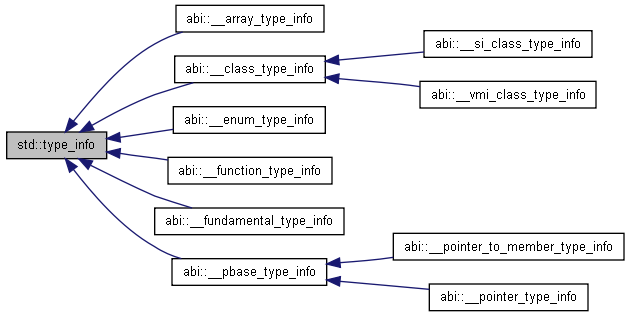
\includegraphics[width=0.9\textwidth]{images/gcc_rtti_hierarchy.png}
\caption{Иерархия производных от \lstinline{std::type_info} классов, используемая в компиляторе GCC.}
\label{fig:gcc_rtti_hierarchy}
\end{figure}


Компилятор GCC, в отличие от MSVC, для хранения информации о типах времени выполнения использует иерархию производных от \lstinline{std::type_info} классов. Описание иерархии этих классов приводится в заголовочном файле \lstinline{<cxxabi.h>}, поставляемом с компилятором GCC, и доступно для использования из любой программы, написанной на Си++. Организация доступа к информации о типах времени выполнения в компиляторе GCC схожа с используемой в MSVC --- для каждого полиморфного класса перед таблицей виртуальных функций помещается указатель на соответствующий ему объект производного от \lstinline{std::type_info} класса, хранящий информацию о типе. Иерархия производных от \lstinline{std::type_info} классов представлена на рис. \ref{fig:gcc_rtti_hierarchy}.

Для классов, не имеющих базовых, используются тип \lstinline{abi::__class_type_info}, не содержащий никакой дополнительной информации по сравнению с \lstinline{std::type_info}. Он является базовым для двух других классов --- \lstinline{abi::__si_class_type_info} и \lstinline{abi::__vmi_class_type_info}. Первый используется для классов, имеющих ровно один невиртуальный публичный базовый класс\footnote{англ. non-virtual public base class --- базовый класс, унаследованный с модификатором \lstinline{public} и без модификатора \lstinline{virtual}.}. По сравнению с \lstinline{std::type_info}, он содержит только одно дополнительное поле - указатель на \lstinline{abi::__class_type_info} соответствующего базового класса. Для всех прочих классов используется тип \lstinline{abi::__vmi_class_type_info}. Описание этого класса представлено на рис. \ref{listing:__vmi_class_type_info}.

\begin{figure}[htb!]
\hspace{2cm}
\begin{minipage}[b]{1cm}
\begin{cplusplus}
class __vmi_class_type_info: public __class_type_info {
public:
  /** #\tl{Атрибуты, отвечающие за множественное и}@
   * #\tl{виртуальное наследование.}@ */
  unsigned int __flags;
  
  /** #\tl{Количество базовых классов.}@ */
  unsigned int __base_count;
  
  /** #\tl{Массив структур, описывающих базовые классы.}@ */
  __base_class_type_info __base_info[1];
};
\end{cplusplus}
\end{minipage}
\caption{Описание класса \lstinline{abi::__vmi_class_type_info}.}
\label{listing:__vmi_class_type_info}
\end{figure}

Для хранения информации о базовых классах используется массив структур типа \lstinline{abi::__base_class_type_info}. Описание этой структуры представлено на рис. \ref{listing:__base_class_type_info}. Используя информацию, предоставляемую этими структурами, можно восстановить полную иерархию полиморфных классов приложения.

\begin{figure}[htb!]
\hspace{2cm}
\begin{minipage}[b]{1cm}
\begin{cplusplus}
struct __base_class_type_info {
public:
  /** #\tl{Указатель на \_\_class\_type\_info базового класса.}@ */
  const __class_type_info *__base_type;
  
  /** #\tl{Поле, хранящее смещение объекта данного класса}@
   * #\tl{внутри экземпляра производного.}@ */
  long __offset_flags;
};
\end{cplusplus}
\end{minipage}
\caption{Описание класса \lstinline{abi::__base_class_type_info}.}
\label{listing:__base_class_type_info}
\end{figure}

\begin{figure}[htb!]
\hspace{2cm}
\begin{minipage}[b]{1cm}
\begin{cplusplus}
class type_info {
public:
  /* ... */
private:
  const char *__type_name;
  /* ... */
};
\end{cplusplus}
\end{minipage}
\caption{Описание класса \lstinline{std::type_info}, используемого компилятором GCC.}
\label{listing:gcc_type_info}
\end{figure}

Так же, как и в случае с компилятором MSVC, возможно восстановление имен классов. Рассмотрим описание класса \lstinline{std::type_info}, представленное на рис. \ref{listing:gcc_type_info}. В поле \lstinline{__type_name} хранится указатель на декорированное имя класса, соответствующего данному объекту класса \lstinline{std::type_info}. Декодирование осуществляется с помощью функции \lstinline{abi::__cxa_demangle}, объявленной в \lstinline{<cxxabi.h>}. Таким образом, компилятор GCC предоставляет возможности по восстановлению иерархий полиморфных классов как минимум такие же, как компилятор MSVC.




\subsection{Получение информации о типах времени выполнения}\label{chapter:rtti_extraction}
Зная описанный выше формат использованных в программе структур, содержащих информацию о типах времени выполнения, можно путем анализа ассемблерного представления программы извлечь из них информацию обо всех полиморфных классах этой программы. С использованием извлеченной информации возможно восстановление иерархии полиморфных классов. Для этого необходимо:

\begin{itemize}
\item Выяснить используемый формат информации о типах времени выполнения.
\item Локализовать структуры, содержащие информацию о типах времени выполнения.
\item Извлечь предоставляемую этими структурами информацию о полиморфных классах.
\item Провести анализ извлеченной информации.
\end{itemize}

Формат структур, содержащих информацию о типах времени выполнения, определяется использованным в компиляторе бинарным интерфейсом приложений. Так как различных бинарных интерфейсов приложений для архитектуры не так много, то, локализовав структуры, содержащие информацию о типах времени выполнения, можно попытаться разобрать их с использованием всевозможных форматов. В случае, если рассматриваются только компиляторы GCC и MSVC, такой способ всегда дает результат в силу того, что форматы информации о типах времени выполнения, используемые этими компиляторами, сильно отличаются.

Также, если определить компилятор, с использованием которого была получена анализируемая программа, и узнать используемый этим компилятором бинарный интерфейс приложений, то можно определить и используемый в анализируемой программе формат структур, содержащих информацию о типах времени выполнения. Компилятор в большинстве случаев можно определить по используемой приложением стандартной библиотеке. Если приложение использует динамически подключаемую стандартную библиотеку, то компилятор определяется по файлу этой библиотеки. Если же используется статически связанная с программой стандартная библиотека, то ее версию и производителя можно выявить с использованием сравнения сигнатур функций. В случае же, если стандартная библиотека приложением не используется, что является редким случаем, можно применить описанный выше переборный метод.

Извлечение информации о полиморфных классах при известном формате и положении структур, содержащих информацию о типах времени выполнения, не представляет проблем. Основная сложность на этом этапе заключается в локализации этих структур.

Так как указатель на структуру, содержащую информацию о типах времени выполнения, всегда предшествует соответствующей таблице виртуальных функций (см. главу \ref{chapter:rtti_in_cpp}), то задача локализации этих структур сводится к задаче поиска таблиц виртуальных функций.




\subsubsection{Локализация информации о типах времени выполнения}\label{chapter:finding_rtti_structures}
Как было сказано в главе \ref{chapter:rtti_extraction}, задача локализации структур, содержащих информацию о типах времени выполнения, может быть сведена к задаче поиска таблиц виртуальных функций. На основе следующих соображений можно построить алгоритм поиска таблиц виртуальных функций:

\begin{itemize}
\item Таблицы виртуальных функций хранятся в сегменте данных.
\item Каждая таблица виртуальных функций представляет собой массив из указателей в сегмент кода.
\item Каждый такой указатель ссылается на начало функции или {\it адаптера}.
\item Из сегмента кода существуют ссылки на первый элемент таблицы виртуальных функций --- адрес первого элемента таблицы используется в конструкторе и деструкторе соответствующего класса.
\item На остальные элементы таблицы виртуальных функций ссылок нет.
\end{itemize}

\begin{figure}[htb!]
\begin{algorithmic}[1]
\STATE $p \gets \textit{DataSegment}_{\textit{start}}$
\WHILE{$p < \textit{DataSegment}_{\textit{end}}$}
    \STATE $\textit{vTableSize} \gets \textit{getVTableSize}(p)$
    \IF{$\textit{vTableSize} \ne 0$}
        \IF {$\textit{isPointerToRtti}(\text{\lstinline{*}}(p - \text{\lstinline{sizeof(void*)}}))$}
            \STATE \textbf{dump} \textit{RTTI structure at} $\text{\lstinline{*}}(p - \text{\lstinline{sizeof(void*)}})$
        \ENDIF
        \STATE $p \gets p + \text{\lstinline{sizeof(void*)}} \cdot \textit{vTableSize}$
    \ELSE
        \STATE $p \gets p + \text{\lstinline{sizeof(void*)}}$
    \ENDIF
\ENDWHILE
\end{algorithmic}
\caption{Алгоритм поиска таблиц виртуальных функций.}
\label{alg:find_vtables}
\end{figure}

\begin{figure}[htb!]
\begin{algorithmic}[1]
\STATE \textbf{function} $\textit{getVTableSize}(p)$
\IF{$\text{\textbf{not}} ~ \textit{isReferenced}(p) ~ \text{\textbf{or not}} ~ \textit{isPointerToFunction}(\text{\lstinline{*}}p)$}
    \RETURN 0
\ELSE
    \STATE $\textit{vTableSize} \gets 1$
    \LOOP
        \IF{$\textit{isReferenced}(p) ~ \text{\textbf{or not}} ~ \textit{isPointerToFunction}(\text{\lstinline{*}}p)$}
            \RETURN $\textit{vTableSize}$
        \ENDIF
        \STATE $\textit{vTableSize} \gets \textit{vTableSize} + 1$
        \STATE $p \gets p + \text{\lstinline{sizeof(void*)}}$
    \ENDLOOP
\ENDIF
\end{algorithmic}
\caption{Описание функции вычисления размера таблицы виртуальных функций.}
\label{alg:getvtablesize}
\end{figure}

Перед таблицей виртуальных функций должен находиться указатель на соответствующую структуру, содержащую информацию о типах времени выполнения, формат которой известен (см. главы \ref{chapter:rtti_in_gcc} и \ref{chapter:rtti_in_msvc}) и накладывает некоторые ограничения на возможные значения ее двоичного представления. Поэтому после локализации таблицы виртуальных функций необходимо также проверить выполнение этих ограничений.

Описание алгоритма поиска структур, содержащих информацию о типах времени выполнения, представлен на рис. \ref{alg:find_vtables}. Этот алгоритм использует функцию $\textit{getVTableSize}$, описание которой приведено на рис. \ref{alg:getvtablesize}. При описании алгоритмов также были использованы следующие функции:
{\centering
\begin{tabularx}{\textwidth}{rcX}
    $\textit{isPointerToRtti}$ & --- & определяет, может ли данный указатель ссылаться на структуру, содержащую информацию о типах времени выполнения. \\
       $\textit{isReferenced}$ & --- & определяет, существуют ли ссылки на данную локацию из сегмента кода. \\
$\textit{isPointerToFunction}$ & --- & определяет, является ли данный указатель указателем на функцию. \\
\end{tabularx}}

Согласно описанным в главах \ref{chapter:rtti_in_msvc} и \ref{chapter:rtti_in_gcc} форматам информации о типах времени выполнения, путем разбора структуры, содержащей информацию о типах времени выполнения для некоторого класса $A$, можно узнать имена всех непосредственные базовых классов для $A$. Тогда, применяя представленный на рис. \ref{alg:find_vtables} алгоритм поиска структур, содержащих информацию о типах времени выполнения, можно путем разбора этих структур восстановить полную иерархию полиморфных классов программы, причем такое восстановление будет корректным.
























\newpage
\section{Восстановление объектных структур данных при декомпиляции при отсутствии информации о типах времени выполнения}\label{chapter:reconstruction_without_rtti}
В связи с тем, что использование информации о типах времени выполнения в программах на языке Си++ считается <<дурным тоном>>, и зачастую используется неправильно \cite{stroustrup93}, сегодня существуют программные продукты, не использующие информацию о типах времени выполнения. В случае, если программа была скомпилирована без информации о типах времени выполнения, для каждого полиморфного класса по-прежнему генерируется таблица виртуальных функций. Вообще говоря, уникальность таблицы для каждого класса не гарантируется, и компилятор может объединить таблицы для двух полиморфных классов \lstinline{Base} и \lstinline{Derived}, если \lstinline{Base} является предком \lstinline{Derived} и при этом \lstinline{Derived} не {\it перекрывает} ни одну из виртуальных функций, объявленных в \lstinline{Base}. Однако в случае, если хотя бы одна из добавленных в \lstinline{Derived} виртуальных функций не являются {\it чисто виртуальной}, компиляторы GCC и MSVC создают для \lstinline{Derived} отдельную таблицу виртуальных функций. 
%Таким образом, если найти все таблицы виртуальных функций, то путем анализа их структуры и входящих в них функций можно восстановить иерархию полиморфных классов программы.

Как было отмечено в главе \ref{chapter:problem}, для корректного восстановления иерархии классов некоторой ассемблерной программы $\bA$, полученной путем компиляции программы на языке Си++ $\bP$, необходимо построить множество классов $\gCa$, и восстановить отношение непосредственного наследования $\leftarrow \; \subseteq \gCa \times \gCa$. В дальнейшем будем рассматривать отношение\footnote{Здесь и далее определения используемых обозначений даны в приложении А.} $\lhd = \enspace \leftarrow^+$. $\lhd$ является отношением строгого частичного порядка, так как оно:
\begin{itemize}
\item Антирефлексивно: $\forall A \in \gCa: \neg (A \lhd A)$;
\item Ассиметрично: $\forall B, D \in \gCa: B \lhd D \Longrightarrow \neg (D \lhd B)$;
\item Транзитивно: $\forall B, C, D \in \gCa: B \lhd C \wedge C \lhd D \Longrightarrow B \lhd D$.
\end{itemize}

Это в частности означает, что отношение $\leftarrow$ восстанавливается по отношению $\lhd$ следующим образом: $\leftarrow \; = \lhd \setminus \lhd \circ \lhd$.

В дальнейшем будем предполагать, что компилятор, с помощью которого была скомпилирована исследуемая программа, известен. Информация о компиляторе могла быть получена как с использованием методов, описанных в главе \ref{chapter:rtti_extraction}, так и из внешних источников.

%Обозначим множество всех таблиц виртуальных функций программы $VTables$. Для удобства введем также отображение $ClassOf: VTables \rightarrow \gC$, возвращающее для каждой таблицы виртуальных функций соответствующий ей класс. Аналогично с введенным на множестве $\gC$ отношением $\leftarrow$, введем отношение $\leftarrow$ и на множестве $VTables$: будем говорить, что таблица виртуальных функций $d$ является непосредственным наследником таблицы виртуальных функций $b$, то есть $b \leftarrow d$, тогда и только тогда, когда $ClassOf(b) \leftarrow ClassOf(d)$.

%Аналогично с отношением $\lhd$ на множестве классов определим это отношение и на множестве таблиц виртуальных функций: $\lhd = \; \leftarrow^+$. Для отношения $\lhd$ на множестве таблиц виртуальных функций будем применять те же термины, что и для отношения $\lhd$ на множестве классов.


\subsection{Обработка множественного наследования}\label{chapter:multiple_inheritance}
Так как для классов, имеющих несколько непосредственных базовых полиморфных классов, компиляторы GCC и MSVC генерируют несколько таблиц виртуальных функций --- по одной таблице на каждую таблицу виртуальных функций каждого непосредственного базового полиморфного класса \cite{gray94, gccabi}, то в общем случае отличить множественное наследование от одиночного оказывается затруднительно. На рис. \ref{fig:multiple_base_example_vtable} представлены сгенерированные компилятором MSVC таблицы виртуальных функций для иерархии классов, представленной на рис. \ref{listing:multiple_base_example}.

\begin{figure}[htb!]
\hspace{2cm}
\begin{minipage}[b]{1cm}
\begin{cplusplus}
class A {
public:
    virtual void a() {/* ... */}
};

class B {
public:
    virtual void b() {/* ... */}
};

class C: public A, public B {
public:
    virtual void a() {/* ... */}
    virtual void b() {/* ... */}
};
\end{cplusplus}
\end{minipage}
\caption{Пример использования множественного наследования в Си++.}
\label{listing:multiple_base_example}
\end{figure}

\begin{figure}[htb!]
\hspace{2cm}
\begin{minipage}[b]{1cm}
\lstinline!const A::`vftable'! \\
\fbox{\lstinline{&A::a(void)}} \\
\\
\lstinline!const B::`vftable'! \\
\fbox{\lstinline{&B::b(void)}} \\
\\
\lstinline!const C::`vftable'{for `A'}! \\
\fbox{\lstinline{&C::a(void)}} \\
\\
\lstinline!const C::`vftable'{for `B'}! \\
\fbox{\lstinline{&C::b(void)}}
\end{minipage}
\caption{Таблицы виртуальных функций, сгенерированные компилятором MSVC для иерархии классов, представленной на рис. \ref{listing:multiple_base_example}.}
\label{fig:multiple_base_example_vtable}
\end{figure}

\begin{figure}[htb!]
\hspace{2cm}
\begin{minipage}[b]{1cm}
\begin{cplusplus}
class B1: public B {
public:
    virtual void b() {/* ... */}
};

class C: public A {
private:
    B1 b;
public:
    virtual void a() {/* ... */}
};
\end{cplusplus}
\end{minipage}
\caption{Модифицированная иерархия наследования.}
\label{listing:multiple_base_example_modified}
\end{figure}

Сравним приведенное на рис. \ref{listing:multiple_base_example_modified} альтернативное описание класса \lstinline{C} c приведенным на рис. \ref{listing:multiple_base_example}. Как видно, альтернативное описание было получено путем переноса метода \lstinline{C::b(void)} из класса \lstinline{C} в производный от \lstinline{B} класс \lstinline{B1}, удаления класса \lstinline{B} из списка базовых классов для класса \lstinline{C}, и добавления нового поля типа \lstinline{B1} в класс \lstinline{C}. При такой организации иерархии множественное наследование было заменено одиночным наследованием с добавлением поля. В результате проведения экспериментов было выяснено, что для иерархий, представленных на рис. \ref{listing:multiple_base_example} и рис. \ref{listing:multiple_base_example_modified}, компилятор MSVC генерирует таблицы виртуальных функций, имеющие одинаковую структуру --- такую же, как на рис. \ref{fig:multiple_base_example_vtable}. Дальнейшее исследование полученных в результате компиляции ассемблерных программ показало, что они эквивалентны в смысле, определенном в \cite{dolgova08}. Такие же результаты были получены и для компилятора GCC.

\begin{figure}[htb!]
\hspace{2cm}
\begin{minipage}[b]{1cm}
\begin{cplusplus}
class B1 {
    /* ... */
public:
    virtual b1() {/* ... */}
};

class B2 {
    /* ... */
public:
    virtual b2() {/* ... */}
};

class D: public B1, public B2 {
    /* ... */
public:
    virtual b2() {/* #\tl{обращение к полям B1}@ */}
};
\end{cplusplus}
\end{minipage}
\caption{Пример иерархии классов, в виртуальных функциях классов которой возможно обращение по отрицательному смещению относительно переданного в функцию указателя \lstinline{this}.}
\label{listing:negative_this_access}
\end{figure}

В некоторых случаях использование множественного наследования можно выявить. Один из таких случаев --- наличие обращения по отрицательному смещению относительно указателя \lstinline{this} в одной из виртуальных функций. Рассмотрим пример, приведенный на рис. \ref{listing:negative_this_access}. Согласно используемым в компиляторах GCC и MSVC бинарным интерфейсам приложений \cite{gray94, gccabi}, объект класса \lstinline{D} будет иметь структуру, представленную на рис. \ref{fig:class_layout}.

\begin{figure}[htb!]
\centering
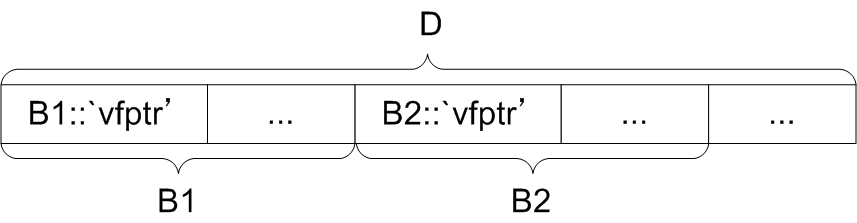
\includegraphics[scale=1.0]{images/class_layout.png}
\caption{Структура объекта класса \lstinline{D}, описанного на рис. \ref{listing:negative_this_access}.}
\label{fig:class_layout}
\end{figure}

При вызове виртуальной функции \lstinline{D::b2} в качестве указателя \lstinline{this} ей будет передан не указатель на начало объекта класса \lstinline{D}, а указатель на начало экземпляра класса \lstinline{B2} внутри этого объекта. Функция \lstinline{D::b2} работает с полями, унаследованными классом \lstinline{D} от \lstinline{B1}, и так как экземпляр класса \lstinline{B1} предшествует экземпляру класса \lstinline{B2} внутри объекта класса \lstinline{D}, как это изображено на рис. \ref{fig:class_layout}, то обращение к этим полям будет производиться по отрицательному смещению относительно переданного в функцию \lstinline{D::b2} указателя \lstinline{this}. Заметим, что в случае одиночного наследования такая ситуация невозможна.

Еще один случай, в котором можно выявить множественное наследование, связан с использованием виртуальных деструкторов. Рассмотрим пример, приведенный на рис. \ref{listing:multiple_base_vdestructor}.

\begin{figure}[htb!]
\hspace{2cm}
\begin{minipage}[b]{1cm}
\begin{cplusplus}
class B1 {
public:
    virtual ~B1() {/* ... */}
};

class B2 {
public:
    virtual ~B2() {/* ... */}
};

class D: public B1, public B2 {
public:
    virtual ~D() {/* ... */}
};
\end{cplusplus}
\end{minipage}
\caption{Пример использования виртуальных деструкторов в иерархии с множественным наследованием.}
\label{listing:multiple_base_vdestructor}
\end{figure}

В данном примере для класса \lstinline{D} генерируется две таблицы виртуальных функций --- по одной для каждого полиморфного базового класса. При этом обе таблицы должны содержать указатель на виртуальный деструктор класса \lstinline{D}. Однако при вызове виртуального деструктора для класса \lstinline{B2}, ему передается указатель не на объект класса \lstinline{D}, а на экземпляр класса \lstinline{B2} внутри объекта класса \lstinline{D}. Поэтому в таблице виртуальных функций класса \lstinline{D}, соответствующей классу \lstinline{B2}, хранится указатель не на виртуальный деструктор класса \lstinline{D}, а на {\it адаптер}, производящий выравнивание переданного указателя \lstinline{this} таким образом, чтобы он указывал на начало объекта класса \lstinline{D}, и передающий управление виртуальному деструктору. Размер полиморфного класса всегда больше нуля, так как объекты такого класса хранят указатель на таблицу виртуальных функций, и поэтому различным полиморфным базовым классам с виртуальными деструкторами соответствуют различные адаптеры. По коду такого адаптера также можно определить смещение базового класса внутри объемлющего. Метод выявления виртуальных деструкторов описан в главе \ref{chapter:destructors}.

Так как большинство иерархий классов используют виртуальные деструкторы, то изложенные выше факты в большинстве случаев дают возможность выявить использование множественного наследования, и определить, какие таблицы виртуальных функций принадлежат одному и тому же классу. В случае отсутствия виртуальных деструкторов можно выявить факт использования множественного наследования, но определить, какие таблицы виртуальных функций принадлежат одному и тому же классу, оказывается затруднительно. Также не смотря на то, что обращение по отрицательному относительно указателя \lstinline{this} смещению подразумевает использование множественного наследования, такое обращение возможно и при использовании одиночного наследования при наложении дополнительных ограничений на параметры функции. В результате проведения экспериментов было выяснено, что в случае отсутствия виртуальных деструкторов, для программы на языке Си++ $\bP$, использующей множественное наследование, и соответствующей ей программы на языке ассемблера $\bA$, возможно построить программу $\bP'$, использующую лишь одиночное наследование, при компиляции которой получается ассемблерная программа $\bA'$, эквивалентная $\bA$. Метод построения такой программы основан на тех же приемах, что были приведены выше в комментариях к рис. \ref{listing:multiple_base_example} и \ref{listing:multiple_base_example_modified}.

Таким образом, восстановление иерархии полиморфных классов можно разбить на два этапа:
\begin{enumerate}
\item Восстановление отношения наследования на множестве таблиц виртуальных функций. Наследование на этом множестве будет одиночным, так как каждой таблице виртуальных функций некоторого класса, использующего множественное наследование, соответствует только одна таблица виртуальных функций одного из базовых классов.
\item Путем анализа виртуальных деструкторов выяснить, какие таблицы виртуальных функций принадлежат одним и тем же классам, и, таким образом, восстановить отношение наследования на множестве полиморфных классов.
\end{enumerate}

На первом этапе восстановления будем считать, что каждой таблице виртуальных функций соответствует отдельный класс, то есть множество всех таблиц виртуальных функций программы на языке ассемблера $\bA$ задает множество всех классов $\gCa$. На втором этапе восстановления иерархии некоторые из классов из $\gCa$ будут объединены в один. Рассмотрим первый этап восстановления.

%Наследование на этом множестве будет одиночным, так как каждой таблице виртуальных функций некоторого класса, использующего множественное наследование, соответствует только одна таблица виртуальных функций одного из базовых классов. Отношение же наследования на множестве таблиц виртуальных функций однозначно задается отношением наследования на множестве классов. Таким образом, если считать, что в программе используется лишь одиночное наследование, что, как было выяснено выше, не противоречит возможности корректного восстановления иерархии классов, то можно считать, что отношения наследования на множестве классов и на множестве таблиц виртуальных функций совпадают, и потому множество всех таблиц виртуальных функций программы на языке ассемблера $\bA$ задает множество всех классов $\gCa$.

%После восстановления иерархии наследования на множестве виртуальных функций, путем анализа виртуальных деструкторов можно выяснить, какие таблицы виртуальных функций принадлежат одним и тем же классам, и, объединив соответствующие им классы из $\gCa$ в один, восстановить также и множественное наследование.



%\subsection{Извлечение информации о структуре иерархии полиморфных классов}
\subsection{Получение информации об отношении наследования}
\label{chapter:info_extraction}
Пусть поиск таблиц виртуальных функций выполнен так, как это описано в главе \ref{chapter:finding_rtti_structures}, но с поправкой на отсутствие информации о типах времени выполнения. Пусть $\gVa^R$ --- множество всех найденных таблиц виртуальных функций. Так как алгоритм поиска таблиц виртуальных функций не отличает массивы из указателей на функции от сгенерированных компилятором таблиц виртуальных функций, то в $\gVa^R$ могут присутствовать элементы, которым не соответствует таблица виртуальных функций, и для которых не существует соответствующего класса в $\gCp$. Пусть $\gVa \subseteq \gVa^R$ --- реальное множество таблиц виртуальных функций. При компиляции разные классы могут разделять одну таблицу виртуальных функций, как это описано в начале главы \ref{chapter:reconstruction_without_rtti}, и потому каждому элементу из $\gVa$ может соответствовать более одного класса из $\gCp$. Для программы на языке Си++ $\bP$ расширим отношение непосредственного наследования $\leftarrow_{\bP}$ на множество $\gVa$. Пусть $\forall b, d \in \gVa: b \leftarrow_{\bP} d \Longleftrightarrow$ для некоторых соответствующих $b$ и $d$ классов $B, D \in \gCp$ выполнено $B \leftarrow_{\bP} D$ и таблица виртуальных функций $d$ класса $D$ соответствует таблице виртуальных функций $b$ класса $B$.

На первом этапе восстановления будем считать, что каждой таблице виртуальных функций соответствует отдельный полиморфный класс, и будем отождествлять понятия <<таблица виртуальных функций>> и <<класс>>. Тогда множество полиморфных классов $\gCa$ однозначно задается множеством восстановленных таблиц виртуальных функций $\gVa^R$, и наследование на множестве $\gCa$ является одиночным, как это описано в конце главы \ref{chapter:multiple_inheritance}. Пусть функция $\Map \in \gCa \rightarrow \gVa \cup \nu$ для класса из $\gCa$ возвращает специальное значение $\nu$, если в $\gVa$ не существует соответствующей ему таблицы виртуальных функций, и соответствующую ему таблицу виртуальных функций в противном случае. Расширим функцию $\Map$ на множество $2^{\gCa}$ следующим образом:
\begin{equation}
\forall \gf \subseteq \gCa: \Map(\gf) = \bigcup_{C \in \gf} \Map(C)\text{.}
\end{equation}

Для восстановления связей между классами рассмотрим бинарное отношение наследования $\lhd$, определенное в главе \ref{chapter:reconstruction_without_rtti}. Для удобства восстановления разложим отношение $\lhd$ на два отношения $<$ и $\sim$ следующим образом:
\begin{align*}
< &= \gCa^2 \setminus \lhd^{-1} \text{,} \\
\sim &= \lhd^= \cup \lhd^{-1} \text{.}
\end{align*}

Иначе говоря:
\begin{align*}
&\forall B, D \in \gCa: (B, D) \in \; < \quad \Longleftrightarrow \enspace \text{$D$ не является предком $B$,} \\
&\forall B, D \in \gCa: (B, D) \in \; \sim \quad \Longleftrightarrow \enspace \text{$D$ и $B$ связаны наследованием.}
\end{align*}

Не сложно проверить, что $\lhd = \: < \cap \sim^{\ne}$. Также заметим, что оба введенных отношения рефлексивны, и при этом $\sim$ симметрично, то есть:
\begin{align*}
&\forall A \in \gCa: A < A \wedge A \sim A \text{,} \\
&\forall B, D \in \gCa: B \sim D \Longrightarrow D \sim B \text{.}
\end{align*}

Информация о структуре иерархии классов может быть записана в виде множества ограничений на отношение $\leftarrow$. При этом каждое ограничение представимо в виде некоторого булева выражения:
\begin{align}
\cR(\leftarrow, C_1, \ldots, C_n)\text{,} &\text{~где~} C_i \in \gCa \text{, или} \label{eq:restrict_type_1} \\
\cR(\leftarrow, \gf_1, \ldots, \gf_n)\text{,} &\text{~где~} \gf_i \subseteq \gCa \text{.} \label{eq:restrict_type_2}
\end{align}

Будем рассматривать такие ограничения $\cR$, для которых выполнено:
\begin{equation}\label{eq:restriction}
\begin{aligned}
\cR(\leftarrow_{\bP}, \Map(C_1), \ldots, \Map(C_n)) \text{,} &\text{~для ограничений вида (\ref{eq:restrict_type_1}), и} \\
\cR(\leftarrow_{\bP}, \Map(\gf_1), \ldots, \Map(\gf_n)) \text{,} &\text{~для ограничений вида (\ref{eq:restrict_type_2}).}
\end{aligned}
\end{equation}

Так как в область значений функции $\Map$ входит $\nu \notin \gVa$, то будем также считать, что выражения вида (\ref{eq:restriction}), в которых встречается $\nu$, всегда истинны.

Далее будут рассмотрены способы построения ограничений, для которых выполнено (\ref{eq:restriction}). Перед тем, как перейти к описанию способов построения таких ограничений, введем некоторые обозначения. Пусть

{\centering
\begin{tabularx}{\textwidth}{rcX}
        $VT_A$ & --- & таблица виртуальных функций класса $A \in \gCa$. \\
      $|VT_A|$ & --- & размер таблицы виртуальных функций класса $A \in \gCa$. \\
      $VT_A^i$ & --- & $i$-я виртуальная функция класса $A \in \gCa$. \\
  $\params(f)$ & --- & параметры функции $f$. \\
$|\params(f)|$ & --- & суммарный размер параметров функции $f$ в байтах. \\
       $\pure$ & --- & обработчик вызова чисто виртуальной функции. \\
   $\executes$ & --- & бинарное отношение <<выполняет>> между множествами функций и выражений. \\
\end{tabularx}}

Будем считать, что если для некоторой функции $f$ и выражения $e$ выполнено $f \enspace \executes \enspace e$, и некоторая функция $g$ вызывает $f$, используя статическое связывание, то есть выполнено $g \enspace \executes \enspace f\text{\lstinline{(/* ... */)}}$, то также выполнено и $g \enspace \executes \enspace e$.




\subsubsection{Анализ таблиц виртуальных функций}\label{chapter:vftable_analysis}
\begin{statement}\label{stmt:first_good}\label{stmt:vtable_size}
Пусть $B, D \in \gCa: |VT_B| < |VT_D|$. Тогда для ограничения $\cR_{\ref{stmt:vtable_size}}^{BD} = B < D$ выполнено (\ref{eq:restriction}).
\end{statement}
В соответствии с правилами наследования Си++ \cite{cpp03}, если для $D$ виртуальных функций определено больше, чем для $B$, то $D$ не может являться предком $B$.
%cpp03[10.3]

\begin{statement}\label{stmt:inherit_pure}
Пусть $B, D \in \gCa$ и $\exists \, i: VT_B^i = \pure \wedge VT_D^i \ne \pure$. Тогда для ограничения $\cR_{\ref{stmt:inherit_pure}}^{BD} = B < D$ выполнено (\ref{eq:restriction}).
\end{statement}
В Си++ невозможно при наследовании {\it перекрыть} некоторую уже определенную в базовом классе виртуальную функцию как чисто виртуальную. Поэтому в указанной выше ситуации $D$ не может быть предком $B$.

\begin{statement}\label{stmt:fsets}
Пусть $A, C \in \gCa$ и $\exists \, i: VT_A^i = VT_C^i \wedge VT_A^i \ne \pure$. Если при компиляции каждое объявление виртуальной функции в $\bP$ породило отдельную функцию в $\bA$, то для ограничения $\cR_{\ref{stmt:fsets}}^{AC} = A \sim^+ C$ выполнено (\ref{eq:restriction}).
\end{statement}
Если в таблицах виртуальных функций двух разных классов записан указатель на одну и ту же функцию, то это означает, что или эта функция была унаследована одним из этих классов от другого, или оба эти класса унаследовали ее от общего базового класса, или в результате оптимизаций эта функция оказалась записанной в таблицах виртуальных функций двух связанных наследованием классов. Пример для последнего случая рассмотрен в комментарии к утверждению \ref{stmt:fsets_2}.

% вот тут мы опять забыли про reinterpret_cast...

Это утверждение опирается на то, что при компиляции каждое объявление функции в исходном файле порождает новую функцию в ассемблерном представлении. Ни компилятор MSVC, ни компилятор GCC не проводят попарного сравнения кода всех функций при сборке исполнимого файла, но при компиляции отдельного исходного файла компилятор MSVC объединяет простые функции с пустым телом или с телом вида \lstinline{return /* const */} в одну. Пусть $\textit{isPrimitive}(f)$ принимает значение <<истина>> только в том случае, когда функция $f$ ассемблерной программы $\bA$ является <<элементарной>> --- достаточно простой для того, чтобы $f$ могла быть получена путем объединения нескольких функций из $\bP$ с одинаковым телом. Путем проведения экспериментов было выяснено, что <<элементарность>> функции $f$ определяется длиной ее ассемблерного представления --- компилятор MSVC не объединяет достаточно большие функции в одну. С использованием $\textit{isPrimitive}$, утверждение \ref{stmt:fsets} можно переписать следующим образом.

\begin{statement}\label{stmt:fsets_1_5}
Пусть $A, C \in \gCa: \exists \, i: VT_A^i = VT_C^i \wedge VT_A^i \ne \pure \wedge \neg \textit{isPrimitive}(VT_A^i)$. Тогда для ограничения $\cR_{\ref{stmt:fsets_1_5}}^{AC} = A \sim^+ C$ выполнено (\ref{eq:restriction}).
\end{statement}

Верно и более общее утверждение.

\begin{statement}\label{stmt:fsets_2}
Пусть для $\gf \subseteq \gCa$, и для некоторых $i \in \Nat$ и функции $f \ne \pure: \neg \textit{isPrimitive}(f)$ выполнено $\forall C \in \gf: VT_C^i = f \, \wedge \, \forall C \in \gCa \setminus \gf: VT_C^i \ne f$. Тогда, если при компиляции не возникает ситуации, когда однажды перекрытая в базовом классе виртуальная функция появляется в таблице виртуальных функций производного класса, то для ограничения $\cR_{\ref{stmt:fsets_2}}^{\gf} = (\gf, \leftarrow \!\! [\gf]) \in \nT(\gf)$, выполнено (\ref{eq:restriction}).
\end{statement}

Заметим, что ограничение $\cR_{\ref{stmt:fsets_2}}^{\gf}$ означает, что сужение заданной отношением $\leftarrow$ иерархии наследования на множество $\gf$ является деревом.

\begin{figure}[htb!]
\centering
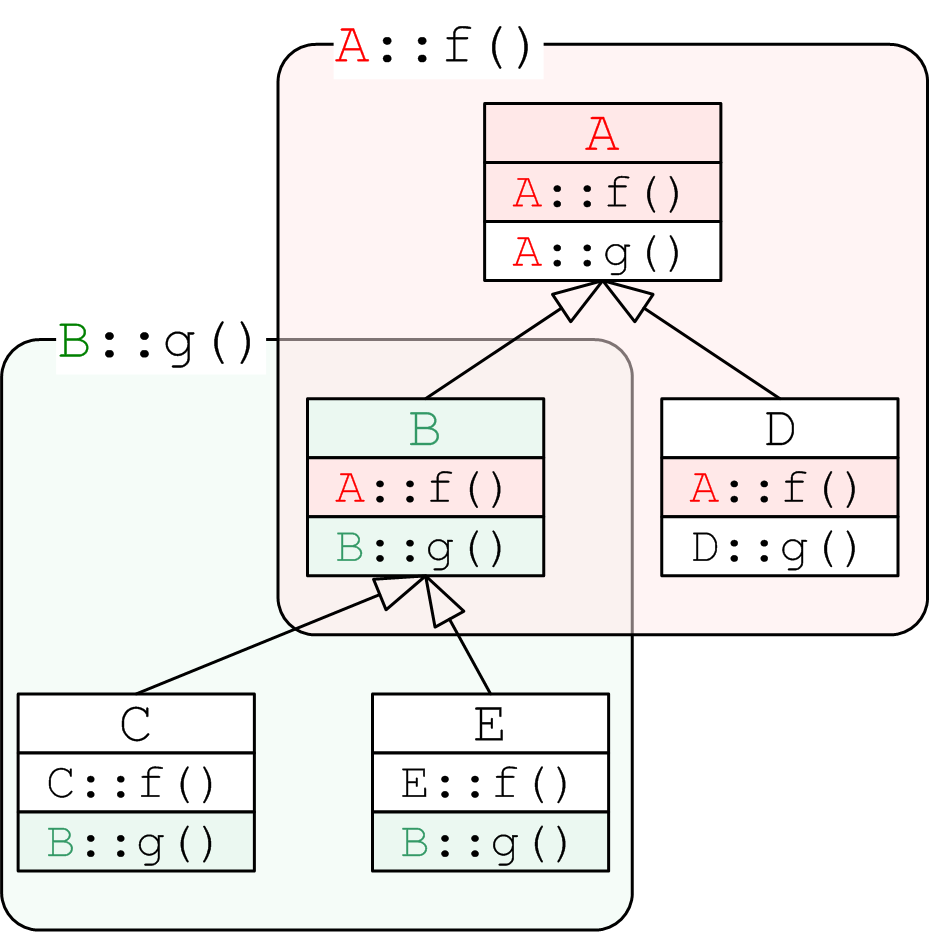
\includegraphics[scale=1.0]{images/fset.png}
\caption{Пример применения утверждения \ref{stmt:fsets_2} к иерархии наследования.}
\label{fig:fsets}
\end{figure}

\begin{figure}[htb!]
\hspace{2cm}
\begin{minipage}[b]{1cm}
\begin{cplusplus}
class A {
public:
    virtual void f() { /* .1. */ }
};

class B: public A {
public:
    virtual void f() { /* .2. */ }
};

class C: public B {
public:
    virtual void f() { A::f(); }
};
\end{cplusplus}
\end{minipage}
\caption{Пример иерархии наследования, для которой дополнительное требование утверждения \ref{stmt:fsets_2} может быть существенным.}
\label{listing:fset_failure}
\end{figure}

\begin{figure}[htb!]
\centering
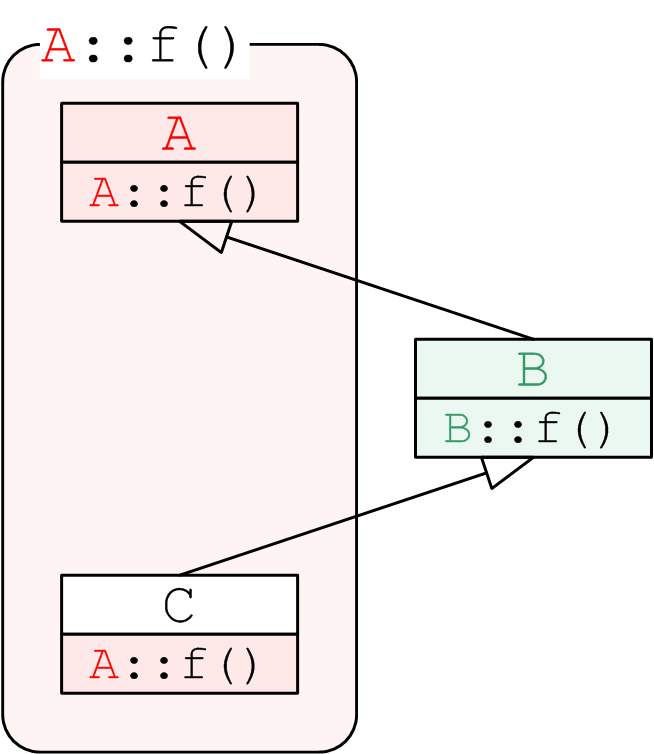
\includegraphics[scale=1.0]{images/fset_failure.png}
\caption{Пример иерархии наследования, для которой дополнительное требование утверждения \ref{stmt:fsets_2} существенно.}
\label{fig:fset_failure}
\end{figure}

На рисунке \ref{fig:fsets} приведен пример применения утверждения \ref{stmt:fsets_2} --- все классы из множества $\{\text{\lstinline{A}}, \text{\lstinline{B}}, \text{\lstinline{D}}\}$ имеют функцию \text{\lstinline{A::f}} на первой позиции в таблице виртуальных функций, и поэтому сужение иерархии наследования на множество $\{\text{\lstinline{A}}, \text{\lstinline{B}}, \text{\lstinline{D}}\}$ является деревом. Утверждение \ref{stmt:fsets_2} справедливо и для множества классов $\{\text{\lstinline{B}}, \text{\lstinline{C}}, \text{\lstinline{E}}\}$, имеющих функцию \text{\lstinline{B::g}} на второй позиции в таблице виртуальных функций.

Утверждение \ref{stmt:fsets_2} опирается на то, что при компиляции не возникает ситуации, когда однажды перекрытая в базовом классе виртуальная функция появляется в таблице виртуальных функций производного класса. Пример такой ситуации представлен на рис. \ref{listing:fset_failure}. При включении оптимизаций компиляторы GCC и MSVC не генерируют тело для функции \lstinline{C::f}, а просто записывают указатель на функцию \lstinline{A::f} в соответствующем месте в таблице виртуальных функций класса \lstinline{C}. Рис. \ref{fig:fset_failure} иллюстрирует применение утверждения \ref{stmt:fsets_2} к иерархии классов, представленной на рис. \ref{listing:fset_failure}. Как видно, применение утверждения в данном случае породило бы ограничение, для которого не выполнено (\ref{eq:restriction}).

Если в утверждении \ref{stmt:fsets_2} не требовать отсутствия ситуаций, подобных изображенной на рис. \ref{listing:fset_failure}, то не для всех полученных с использованием этого утверждения ограничений будет выполнено (\ref{eq:restriction}). Однако так как ситуации, подобные изображенной на рис. \ref{listing:fset_failure}, встречаются достаточно редко, то ограничения, для которых не выполняется (\ref{eq:restriction}), можно в случае возникновения конфликтов обработать отдельно.



\subsubsection{Анализ параметров виртуальных функций}\label{chapter:param_analysis}
\begin{statement}\label{stmt:param_size}
Пусть $A, C \in \gCa: \exists \, i: VT^A_i \ne \pure \wedge VT^C_i \ne \pure \wedge |\params(VT^A_i)| \ne |\params(VT^C_i)|$. Тогда для ограничения $\cR_{\ref{stmt:param_size}}^{AC} = \neg (A \sim C)$ выполнено (\ref{eq:restriction}).
\end{statement}

Согласно правилам наследования Си++, виртуальная функция производного класса должна иметь тот же список параметров, что и перекрываемая ею виртуальная функция базового класса \cite{cpp03}.
%cpp[10.3:2]

Используя методы статического анализа типов можно улучшить точность ограничений, порождаемых приведенным выше утверждением, сравнивая также восстановленные типы параметров, а не только их размер. Однако это требует реализации статического анализа типов, и может привести к проблемам в случае, когда в исходной программе используются структуры данных \lstinline{union}, или оператор \lstinline{reinterpret_cast<>}.

Также проблемы могут возникнуть, если пытаться восстановить суммарный размер параметров, анализируя обращения к стеку. Рассмотрим две функции, представленные на рисунке \ref{listing:param_size}.

\begin{figure}[htb!]
\hspace{2cm}
\begin{minipage}[b]{1cm}
\begin{cplusplus}
int a(int p0, int p1) {
    return p0;
}

int b(int p0, int p1) {
    return p1;
}
\end{cplusplus}
\end{minipage}
\caption{Пример функций, для которых нельзя восстановить суммарный размер параметров путем анализа обращений к стеку.}
\label{listing:param_size}
\end{figure}

Так как в каждой из функций один из аргументов не используется, то независимо от порядка передачи параметров, одна из функций будет обращаться в стек по большему смещению относительно {\tt esp}, чем другая. То есть, даже вычислив максимальное смещение относительно {\tt esp}, по которому происходило обращение к стеку внутри функции, нельзя с уверенностью сказать, что аргументов с большим смещением нет.

Если используется соглашение о вызовах, в котором очисткой стека занимается вызываемая сторона, то суммарный размер параметров определяется по эпилогу функции. В компиляторе MSVC для виртуальных функций по умолчанию используется соглашение \lstinline{thiscall}, обладающее этим свойством. В компиляторе GCC по умолчанию используется стандартное соглашение о вызовах Си, в котором очисткой стека занимается вызывающая сторона, и поэтому для программ, скомпилированных компилятором GCC, такой метод в большинстве случаев неприменим. Также стоит отметить, что для функций, не имеющих аргументов, как при использовании соглашения о вызовах \lstinline{thiscall}, так и при использовании стандартного соглашения о вызовах Си, генерируется один и тот же эпилог. В случае же наличия аргументов эпилоги отличаются, и используемый тип соглашения о вызовах можно определить.

С учетом всего вышесказанного, будем считать суммарный размер параметров определенным только для функций, использующих соглашение о вызовах, в котором очисткой стека занимается вызываемая функция.

\if 0
Заметим также, что верно и более общее утверждение.

\begin{statement}\label{stmt:param_size_2}
Пусть $A, C \in \gCa: \exists \, i: VT^A_i \ne \pure \wedge VT^C_i \ne \pure \wedge |\params(VT^A_i)| \ne |\params(VT^C_i)|$. Тогда для ограничения:
\begin{equation*}
\cR_{\ref{stmt:param_size_2}}^{AC} = \neg (A \sim^+ C) \vee \forall B \in \gCa: B \lhd A \wedge B \lhd C \Rightarrow |VT^B| < i
\end{equation*}
выполнено (\ref{eq:restriction}).
%\begin{equation*}
%\begin{aligned}
%&\neg (\Map(A) \sim^+ \Map(C)) \vee \\
%&\forall B \in \gCa: \Map(B) = \text{\lstinline{void}~} \vee \\
%&\quad (\Map(B) \lhd \Map(A) \wedge \Map(B) \lhd \Map(C) \Rightarrow |VT^B| < i)
%\end{aligned}
%\end{equation*}
\end{statement}

Действительно, если $i$-е функции в таблицах виртуальных функций классов $A$ и $C$ имеют различные размеры параметров, то это означает, что либо $A$ и $C$ не связаны наследованием и не имеют общих предков, либо для всех их общих предков $i$-я виртуальная функция не определена.
\fi



\subsubsection{Анализ вызовов виртуальных функций}\label{chapter:vcalls}
\begin{statement}\label{stmt:vcall}
Пусть $B, D \in \gCa: \exists \, i, j: VT_D^i \enspace \executes \enspace \text{\lstinline{this->}}VT_B^j\text{\lstinline{(...)}} \wedge VT_D^j \ne VT_B^j$. Тогда если в программе $P$ для приведения типов, не связанных наследованием, не используется преобразование \lstinline{reinterpret_cast<>}, или подобное ему, то для ограничения $\cR_{\ref{stmt:vcall}}^{BD} = B \lhd D$ выполнено (\ref{eq:restriction}).
\end{statement}

Если метод $m_D$ класса $D$ вызывает метод $m_B$ класса $B$ для того же объекта, для которого он был вызван сам (то есть для \lstinline{this}), то $m_B$ должен быть определен либо в самом классе $D$, либо в одном из его предков. Конечно, возможен также вариант с использованием оператора \lstinline{reinterpret_cast<>} --- например, $m_D$ может вызывать метод $m_B$ следующим образом: \lstinline{reinterpret_cast<}$B$\lstinline{*>(this)->}$m_B$, однако такие конструкции зачастую лишены смысла и в реальном коде встречаются редко. Поэтому аналогично с утверждением \ref{stmt:fsets_2}, требование отсутствия в программе $\bP$ приведения типов, не связанных наследованием, с использованием преобразования \lstinline{reinterpret_cast<>}, или подобного ему, можно опустить, и в случае возникновения конфликтов обработать отдельно ограничения, для которых не выполняется (\ref{eq:restriction}).

Если $m_B$ является виртуальной функцией, перекрытой в классе $D$, то остается только один вариант --- $B$ является предком $D$. При этом подразумевается, что при вызове виртуальной функции $m_B$ используется {\it статическое связывание}, потому как лишь в этом случае на этапе статического анализа известно, какая функция будет вызвана.

Для того, чтобы определить, действительно ли происходит вызов функции $VT_B^j$ для текущего объекта, необходимо знать способ передачи указателя \lstinline{this} в функции $VT_D^i$ и $VT_B^j$. Зная способ передачи указателя \lstinline{this} в функцию $VT_D^i$, можно провести анализ потока данных и для каждой инструкции в теле функции определить множество регистров и локаций памяти, в которых хранятся копии указателя \lstinline{this}. Используя построенные множества, и зная способ передачи указателя \lstinline{this} в функцию $VT_B^j$, можно определить, действительно ли она вызывается для текущего объекта.

Способ передачи указателя \lstinline{this} зависит от используемого функцией соглашения о вызовах. Используемые компиляторами GCC и MSVC соглашения о вызовах описаны в таблице \ref{fig:calling_conv}. По умолчанию и компилятор GCC, и компилятор MSVC используют соглашение о вызовах \lstinline{thiscall}.

%!!! перенести в обзор?

\begin{figure}[htb!]
\begin{tabular}{| l | l | l |}
\hline
Соглашение о вызовах & Очистка стека & Передача указателя {\color{keywordcolor}\textbf{this}} \\
\hline
MSVC cdecl & \multirow{2}{*}{Вызывающая функция} & \multirow{2}{*}{Первый параметр в стеке} \\
GCC cdecl & & \\
\hline
MSVC fastcall & \multirow{2}{*}{Вызывающая функция} & \multirow{2}{*}{регистр {\tt ECX}} \\
GCC fastcall & & \\
\hline
MSVC stdcall & \multirow{2}{*}{Вызываемая функция} & \multirow{2}{*}{Первый параметр в стеке} \\
GCC stdcall & & \\
\hline
MSVC thiscall & Вызываемая функция & регистр {\tt ECX} \\
\hline
GCC thiscall & Вызывающая функция & Первый параметр в стеке \\
\hline
GCC regparm & & регистр {\tt EAX} \\
\hline
\end{tabular}
\caption{Соглашения о вызовах, используемые компиляторами GCC и MSVC.}
\label{fig:calling_conv}
\end{figure}

Из таблицы \ref{fig:calling_conv} видно, что определение используемого функцией соглашения о вызовах по ее телу представляет некоторые сложности. Конечно, можно считать, что используется соглашение о вызовах \lstinline{thiscall}, что в большинстве случаев является правдой, однако такое предположение верно не всегда, и это может привести к неверным результатам. Однозначно выявить можно только использование соглашения о вызовах \lstinline{stdcall}, которое определяется по эпилогу функции. Однако на практике соглашение о вызовах \lstinline{stdcall} в программах на Си++ используется довольно редко.

В случае использования компилятора MSVC, виртуальной функции в регистре {\tt ECX} нельзя передать ничего кроме указателя \lstinline{this}, и поэтому если внутри функции происходит косвенное обращение к памяти с использованием значения, переданного в регистре {\tt ECX}, то это означает, что в {\tt ECX} был передан указатель \lstinline{this}. Так как компилятор MSVC по умолчанию использует соглашение о вызовах \lstinline{thiscall}, передающее указатель \lstinline{this} в регистре {\tt ECX}, то во многих случаях используемый способ передачи указателя \lstinline{this} можно определить.

Будем применять утверждение \ref{stmt:vcall} только в случаях, когда для функций $VT_D^i$ и $VT_B^j$, с использованием приведенных выше соображений, был восстановлен способ передачи указателя \lstinline{this}.




\subsubsection{Анализ виртуальных деструкторов}\label{chapter:destructors}
Сначала рассмотрим, какие действия должен производить деструктор:

\begin{itemize}
%% \renewcommand{\labelenumii}{(\alph{enumii})}
\item Выполнить заданный программистом в теле деструктора код.
\item Вызвать деструкторы для всех неунаследованных полей.
\item Вызвать деструкторы для всех базовых классов. При вызове деструктора какого-либо базового класса должен использоваться указатель на таблицу виртуальных функций этого класса. Это означает, что в деструкторе указатель на таблицу виртуальных функций будет несколько раз перезаписываться разными значениями, соответствующими различным базовым классам, как это представлено на рис. \ref{listing:destructor}.
\end{itemize}

То есть реальный деструктор --- это функция, сгенерированная компилятором, и написанный программистом код тела деструктора является лишь ее частью.

\begin{figure}[htb!]
\hspace{2cm}
\begin{minipage}[t]{0.1\textwidth}
\vspace{0pt}
\raggedleft

\includegraphics[scale=0.8]{images/destructor.png}
\end{minipage}
\hspace{0.5cm}
\begin{minipage}[t]{0.4\textwidth}
\vspace{0pt}
\raggedright
\begin{cplusplus}[emph={D}, emphstyle=\color{red}, emph={[2]B}, emphstyle={[2]\color{mygreen}}]
D::`destructor'() {
  this->`vfptr' = &D::`vftable';
  this->~D();

  /* ... */

  this->`vfptr' = &B::`vftable';
  this->~B();
}
\end{cplusplus}
\end{minipage}
\caption{Общая схема работы деструктора.}
\label{listing:destructor}
\end{figure}

При создании иерархий классов практически во всех случаях используется виртуальный деструктор --- он дает возможность единообразно уничтожать созданные объекты, при этом не беспокоясь о совместимости существующего кода с новыми классами, которые возможно будут добавлены в будущем. Более того, компилятор GCC даже выдает предупреждение в случае отсутствия виртуального деструктора в полиморфном базовом классе. При использовании виртуального деструктора объекты иерархии обычно создаются с помощью оператора \lstinline{new}, и уничтожаются с использованием оператора \lstinline{delete}. Но использование оператора \lstinline{delete} несет в себе некоторые проблемы. Рассмотрим пример, представленный на рис. \ref{listing:operator_delete}.

\begin{figure}[htb!]
\hspace{2cm}
\begin{minipage}[b]{1cm}
\begin{cplusplus}
struct V {
    virtual ~V();
};

struct W: V {
    void operator delete(void*);
};
\end{cplusplus}
\end{minipage}
\caption{Пример переопределения оператора \lstinline{delete} для класса с виртуальным деструктором.}
\label{listing:operator_delete}
\end{figure}

% [12.4:11]
Согласно правилам Си++ \cite{cpp03}, при вызове оператора \lstinline{delete} для объекта класса \lstinline{V} память должна быть освобождена с помощью глобального оператора \lstinline{::operator delete(void*)}, в то время как для объекта класса \lstinline{W} должен использоваться \lstinline{W::operator delete(void*)}. Так как в месте вызова виртуального деструктора фактический класс уничтожаемого объекта неизвестен, то невозможно определить, какой оператор \lstinline{delete} необходимо вызывать. Поэтому как компилятор GCC, так и компилятор MSVC вместо указателя на деструктор хранят в таблице виртуальных функций указатель на так называемый <<освобождающий деструктор>>\footnote{англ. deleting destructor.}, который в случае необходимости освобождает память с помощью соответствующего оператора \lstinline{delete}.

И в компиляторе GCC, и в компиляторе MSVC код освобождающего деструктора имеет вполне определенную структуру, и может быть идентифицирован с помощью сравнения сигнатур. Теперь, когда место освобождающего деструктора в таблице виртуальных функций определено, можно сформулировать следующее утверждение:

\begin{statement}\label{stmt:destructors}\label{stmt:last_good}
Пусть $B, D \in \gCa: D \text{\lstinline{::~}} \! D \enspace \executes \enspace \text{\lstinline{this->`vfptr'}}\text{~\lstinline{= &}}VT_B$, где поле \lstinline{`vfptr'} хранит указатель на таблицу виртуальных функций. Тогда для ограничения $\cR_{\ref{stmt:destructors}}^{BD} = B \lhd D$ выполнено (\ref{eq:restriction}).
\end{statement}

Казалось бы, это утверждение будет выполнено для всех классов, являющихся предками $D$, однако из-за примененных компилятором оптимизаций это может оказаться не так. Эксперименты с компиляторами GCC и MSVC показали, что в случае использования пустых деструкторов в результате оптимизаций компилятор удаляет последовательные перезаписи поля \lstinline{this->`vfptr'}, оставляя лишь последнюю. Так как в последнюю очередь всегда вызывается деструктор базового класса всей иерархии, то как минимум для него утверждение будет выполнено. Если же у $D$ нет базовых классов, то перезапись поля \lstinline{this->`vfptr'} будет произведена только один раз --- указателем на $VT_D$.

Для того, чтобы определить, действительно ли происходит присваивание вида \lstinline{this->`vfptr'}\lstinline{ = &}$VT_B$, необходимо знать способ передачи указателя \lstinline{this} освобождающему деструктору, и провести анализ потока данных. Как было сказано в главе \ref{chapter:vcalls}, способ передачи указателя \lstinline{this} зависит от используемого освобождающим деструктором соглашения о вызовах.

В компиляторе MSVC, независимо от установленного соглашения о вызовах по умолчанию, для освобождающего деструктора всегда используется соглашение о вызовах \lstinline{thiscall}. В компиляторе GCC используемое для освобождающих деструкторов соглашение о вызовах зависит от установленных по умолчанию атрибутов функций. Так как параметры и структура освобождающего деструктора известны, и различных соглашений о вызовах, используемых компилятором GCC, не так много (см. главу \ref{chapter:vcalls}), то используемое соглашение о вызовах можно определить на этапе сравнения сигнатур.





\subsubsection{Ненадежные источники информации}\label{chapter:unreliable}
Отличительная особенность ограничений, получаемых с использованием описанных выше утверждений --- это их <<надежность>>. Даже при ослабленных требованиях, для большинства встречающихся на практике программных продуктов вероятность получить с их использованием ограничения, для которых не выполнено (\ref{eq:restriction}), близка к нулю. Но существуют и другие источники информации, которые дают ограничения, для которых (\ref{eq:restriction}) не выполняется лишь в небольшом проценте случаев. Приведем несколько примеров таких источников информации.

Пусть $\textit{MaxThisAccessOffset}_A$ --- максимальное смещение относительно указателя \lstinline{this}, по которому происходит обращение к памяти в виртуальных функциях класса $A$, а также в функциях, вызываемых из виртуальных. Пусть $B, D \in \gCa: \textit{MaxThisAccessOffset}_B < \textit{MaxThisAccessOffset}_D$. Тогда для ограничения $\cR_?^{BD} = B < D$ с большой вероятностью выполнено (\ref{eq:restriction}).

Действительно, при наследовании в большинстве случаев добавляется дополнительная функциональность, и для реализации этой функциональности зачастую требуется хранение некоторой дополнительной информации. Эта дополнительная информация добавляется к классу в форме полей, которые затем используются в виртуальных функциях. Из того факта, что добавленные в производном классе поля всегда имеют большее смещение, чем унаследованные \cite{gray94, gccabi}, напрямую следует приведенное выше соображение. Однако в силу того, что для встречающихся на практике программ это соображение не всегда выполнено, его нельзя напрямую использовать для восстановления отношения $<$.

Еще одним примером ненадежного источника информации может служить утверждение \ref{stmt:vcall}, применяемое не только к функциям, для которых используемый метод передачи указателя \lstinline{this} может быть однозначно восстановлен, но и для всех остальных в предположении, что используется соглашение о вызовах по умолчанию.





























\subsection{Восстановление одиночного наследования}\label{chapter:full_sing_inhr_rec}
Как было сказано в главе \ref{chapter:info_extraction}, наследование на множестве классов $\gCa$ является одиночным. В случае использования только одиночного наследования, любое множество классов может быть представлено в виде нескольких деревьев наследования. Каждое дерево наследования является корневым деревом, причем ребра этого дерева заданы отношением непосредственного наследования.

В главе \ref{chapter:destructors} было отмечено, что для каждого класса $D$, принадлежащего некоторому дереву наследования, корнем которого является класс $B$, имеющий виртуальный деструктор, в результате применения утверждения \ref{stmt:destructors} будет получено ограничение $\cR_{\ref{stmt:destructors}}^{BD} = B \lhd D$. Таким образом, с использованием утверждения \ref{stmt:destructors} можно восстановить множество вершин любого дерева наследования с виртуальным деструктором, а таковых, как было отмечено в главе \ref{chapter:destructors}, большинство. В случае же отсутствия виртуального деструктора, множество вершин дерева наследования можно восстановить с использованием утверждения \ref{stmt:fsets}. Таким образом, множество $\gCa$ можно разбить на несколько непересекающихся подмножеств, каждое из которых будет задавать отдельное дерево наследования. С каждым из таких подмножеств можно работать отдельно, и поэтому, для упрощения дальнейших рассуждений, будем считать, что все классы из множества $\gCa$ принадлежат одному дереву наследования.

В этом случае восстановление иерархии классов подразумевает построение дерева наследования $T \in \nT^R(\gCa)$, а перечисленные выше источники информации о структуре иерархии определяют ограничения, которым это дерево должно удовлетворять. Пусть $\gR \subset \nT^R(\gCa) \rightarrow \{0, 1\}$ --- множество всех ограничений, полученных из утверждений \ref{stmt:vtable_size}, \ref{stmt:inherit_pure}, \ref{stmt:fsets_2}, \ref{stmt:param_size}, \ref{stmt:vcall} и \ref{stmt:destructors}, а $\gR_? \subset \nT^R(\gCa) \rightarrow \{0, 1\}$ --- множество всех ограничений, полученных из ненадежных источников информации, как это описано в главе \ref{chapter:unreliable}. В $\gR$ также входят ограничения, полученные из утверждений \ref{stmt:fsets_2} и \ref{stmt:vcall} в предположении о том, что дополнительные требования этих утверждений всегда выполнены. Это означает, что некоторые из ограничений из $\gR$ могут не выполняться.

Тогда задачу построения необходимого корневого дерева можно представить как задачу максимизации функции $\cF \in \nT^R(\gCa) \rightarrow \Rat \times \Rat$, определенной следующим образом:
\begin{equation}
\forall T \in \nT^R(\gCa): \cF(T) = (\sum_{\cR \in \gR} \cR(T), \sum_{\cR \in \gR_?} \cR(T))\text{,}
\end{equation}
где отношение $<$ на $\Rat \times \Rat$ определено следующим образом:
\begin{equation}
\forall (a_1, b_1), (a_2, b_2) \in \Rat \times \Rat: (a_1, b_1) < (a_2, b_2) \Longleftrightarrow a_1 < a_2 \vee (a_1 = a_2 \wedge b_1 < b_2)\text{.}
\end{equation}
Так как различные ограничения из $\gR_?$ могут иметь различную <<степень надежности>>, то при вычислении значения функции $\cF(T)$ возможно применение весовых коэффициентов.

При такой постановке задачи можно использовать ограничения произвольной формы, но при этом точное решение будет возможно получить лишь переборными методами. Приближенное же решение для задачи, поставленной в такой форме, можно получить, использовав метод генетического программирования. В работе \cite{palmer94} было предложено представление деревьев, которое дает хорошие результаты в применении к методам генетического программирования. Подобное представление может быть применено и для поставленной выше задачи.

Метод генетического программирования не всегда находит лучшее решение. С другой стороны, известно, что с большой вероятностью существует дерево наследования, удовлетворяющее всем ограничениям из $\gR$. Введем обозначение:
\begin{equation}
\begin{aligned}
& \isSol \in \nT^R(\gCa) \times 2^{\nT^R(\gCa) \rightarrow \{0, 1\}} \rightarrow \{0, 1\} \text{,}\\
& \forall T \in \nT^R(\gCa), \gR \in 2^{\nT^R(\gCa) \rightarrow \{0, 1\}}: \isSol(T, \gR) \Longleftrightarrow \forall \cR \in \gR: \cR(T)\text{.}
\end{aligned}
\end{equation}

Тогда, если не рассматривать ограничения из $\gR_?$, то в предположении, что все ограничения из $\gR$ могут быть выполнены, поставленная выше задача преобразуется в:
\begin{equation}\label{eq:problem}
\text{Найти~} T \in \nT^R(\gCa): \isSol(T, \gR)
\end{equation}

Так как возможна ситуация, что некоторые из ограничений из $\gR$ могут быть невыполнимы, и потому решения задачи \ref{eq:problem} может не существовать, необходимо построить алгоритм, который будет строить дерево наследования, удовлетворяющее как можно большему количеству ограничений из $\gR$, то есть множеству ограничений $\gR' \subseteq \gR$ такому, что:
\begin{equation}\label{eq:relaxed_gr}
\isSol(T, \gR') \wedge \forall \cR \in \gR \setminus \gR': \nexists T \in \nT^R(\gCa): \isSol(T, \gR' \cup \{\cR\})
\end{equation}

То есть представленный алгоритм должен решать следующую задачу:
\begin{equation}\label{eq:relaxed_problem}
\text{Найти~} \gR' \subseteq \gR, T \in \nT^R(\gCa): \text{~для $\gR'$ выполнено \ref{eq:relaxed_gr}}
\end{equation}



\subsubsection{Алгоритм построения частичного решения задачи восстановления одиночного наследования}\label{chapter:part_single_inher_rec}
Для каждой функции $f$ такой, что $\exists A \in \gCa, i \in \Nat: VT_A^i = f$ построим множество $\gf \subseteq \gCa: \forall C \in \gCa: C \in \gf \Longleftrightarrow VT_C^i = f$. Применяя к этому множеству утверждение \ref{stmt:fsets_2}, и учитывая то, что все ограничения, порожденные этим утверждением, принадлежат множеству $\gR$, получаем:
\begin{equation}\label{eq:is_sol_req}
\forall T \in \nT^R(\gCa): \isSol(T, \gR) \Longrightarrow T[\nT][\gf] \in \nT(\gf) \text{,}
\end{equation}
то есть для того, чтобы дерево $T$ являлось решением задачи (\ref{eq:problem}), необходимо, чтобы его сужение на множество $\gf$ также являлось деревом. Пусть $\gF$ --- множество всех таких множеств $\gf$. Введем обозначение:
\begin{equation}\label{eq:is_partial_solution}
\begin{aligned}
& \isPartSol \in \nT(\gCa) \times 2^{2^{\gCa}} \rightarrow \{0, 1\} \text{,}\\
& \forall T \in \nT(\gCa), \gF \in 2^{2^{\gCa}}: \isPartSol(T, \gF) \Longleftrightarrow \forall \gf \in \gF: T[\gf] \in \nT(\gf)\text{.}
\end{aligned}
\end{equation}

Из (\ref{eq:is_sol_req}) и (\ref{eq:is_partial_solution}) следует:
\begin{equation}\label{eq:is_sol_req_2}
\forall T \in \nT^R(\gCa): \isSol(T, \gR) \Longrightarrow \isPartSol(T[\nT], \gF) \text{,}
\end{equation}
то есть $\isPartSol(T[\nT], \gF)$ является необходимым условием того, что дерево $T$ является решением задачи (\ref{eq:problem}). Будем говорить, что если выполнено $\isPartSol(T[\nT], \gF)$, то дерево $T$ является частичным решением задачи (\ref{eq:problem}).

Пусть
\begin{equation}\label{eq:f_closure_def}
\gFc = \bigcup_{\gF' \subseteq \gF} \left\{ \bigcap_{\gf \in \gF'} \gf \right\} \text{,}
\end{equation}
то есть $\gF^{\cap}$ --- множество всевозможных пересечений множеств из $\gF$. Оценим количество элементов в множестве $\gFc$. Для этого сначала докажем следующую лемму:



\vspace{1cm}
\begin{lemma}\label{lemma:tree_subdivision}
Для любого конечного множества $X$, в любом дереве $T \in \nT(X)$ можно выбрать вершину $x \in X$ таким образом, что при удалении этой вершины и всех инцидентных ей ребер из дерева $T$, это дерево распадется на несколько деревьев, в каждом из которых будет не более $\left\lfloor\frac{|X|}{2}\right\rfloor$ вершин.
\end{lemma}
\begin{proof}
Пусть для некоторого дерева $T$ такую вершину выбрать нельзя, то есть для любой вершины $x \in X$ при ее удалении из дерева $T$, это дерево распадается на несколько поддеревьев, в одном из которых содержится более $\left\lfloor\frac{|X|}{2}\right\rfloor$ вершин. Таких поддеревьев не может быть два, так как иначе в них суммарно содержалось бы более $|X|$ вершин. Обозначим множество вершин такого поддерева, соответствующего вершине $x$, через $V_x$. В множестве $V_x$ содержится ровно одна вершина, инцидентная $x$ в дереве $T$. Обозначим эту вершину $x'$. Тогда возможны два варианта:

\begin{figure}[htb!]
\centering
\begin{minipage}[b]{6cm}
\centering
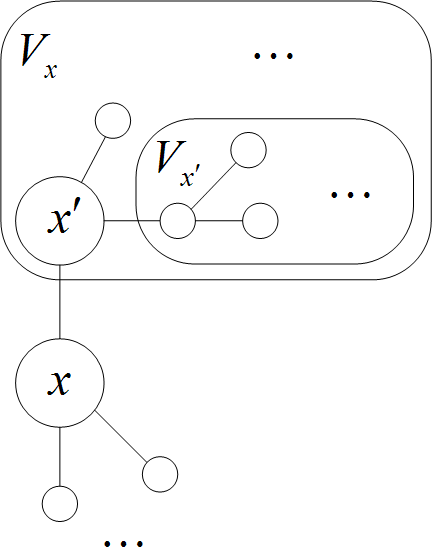
\includegraphics[scale=1.0]{images/tree_division.png}
\caption{Вариант $x \notin V_{x'}$.}
\label{fig:tree_division}
\end{minipage}
\hspace{0.5cm}
\begin{minipage}[b]{6cm}
\centering
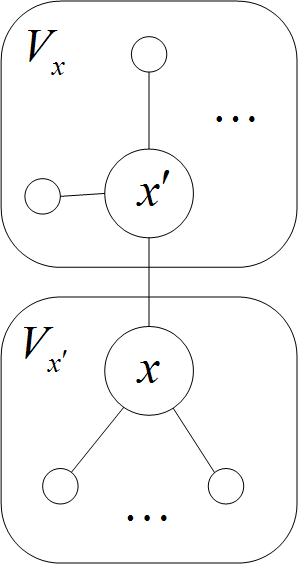
\includegraphics[scale=1.0]{images/tree_division_2.png}
\caption{Вариант $x \in V_{x'}$.}
\label{fig:tree_division_2}
\end{minipage}
\end{figure}

\begin{enumerate}
\item $x \notin V_{x'}$, рис. \ref{fig:tree_division}. В этом случае можно взять $x = x'$ и повторить приведенные выше рассуждения. В силу конечности множества $V_{x'}$, когда-нибудь будет верно, что:
\item $x \in V_{x'}$, рис. \ref{fig:tree_division_2}. В этом случае $V_{x'} \cap V_x = \emptyset$, и $|V_{x'}| + |V_x| > |X|$, что невозможно.
\end{enumerate}
Полученное противоречие завершает доказательство леммы.
\end{proof}
\vspace{1cm}



С использованием леммы \ref{lemma:tree_subdivision} оценим количество элементов в множестве $\gFc$.



\vspace{1cm}
\begin{lemma}\label{lemma:f_closure_size}
Если $k$ --- максимальное количество функций в таблицах виртуальных функций классов из некоторого множества классов $\gC$, $\gF \subseteq 2^{\gC}$, $n = |\gC|$, и $\exists T \in \nT(\gC): \isPartSol(T, \gF)$, то $|\gFc| \le 2n^{k + \log_2{3}}$.
\end{lemma}
\begin{proof}
%Для каждого класса из $\gC$ определено не более $k$ виртуальных функций, и поэтому каждый класс может принадлежать не более чем $k$ различным множествам из $\gF$. Это в частности означает, что:
%\begin{equation}\label{eq:gf_size}
%|\gF| \le nk
%\end{equation}

Пусть $\psi(\gF) = |\gFc|$, а $\nF_k(\gC) \subseteq 2^{2^{\gC}}$ --- множество всевозможных $\gF \subseteq 2^{\gC}$ таких, что каждый элемент из $\gC$ принадлежит не более чем $k$ различным множествам из $\gF$, и $\exists T \in \nT(\gC): \isPartSol(T, \gF)$. Тогда определим функцию $\phi$ следующим образом:
\begin{equation}\label{eq:phi_definition}
\phi(n, k) = \max_{\gF \in \nF_k(\gC) \wedge |\gC| = n} \psi(\gF) \text{.}
\end{equation}

Для функции $\phi$ выполнено:
\begin{equation}\label{eq:phi_additive}
\phi(n_1, k) + \phi(n_2, k) \le \phi(n_1 + n_2, k)\text{.}
\end{equation}

Действительно, для любых двух множеств
\begin{equation}
\begin{aligned}
\gF_1 &\in \nF_k(\gC_1): |\gC_1| = n_1 \text{,} \\
\gF_2 &\in \nF_k(\gC_2): |\gC_2| = n_2 \wedge \gC_1 \cap \gC_2 = \emptyset \text{,}
\end{aligned}
\end{equation}
и деревьев
\begin{equation}\label{eq:t1_t2_def}
\begin{aligned}
T_1 &\in \nT(\gC_1): \isPartSol(T_1, \gF_1) \text{,} \\
T_2 &\in \nT(\gC_2): \isPartSol(T_2, \gF_2) \text{,}
\end{aligned}
\end{equation}
можно взять $T$ --- дерево, полученное из деревьев $T_1$ и $T_2$ добавлением ребра, соединяющего вершину $A$ дерева $T_1$ с вершиной $C$ дерева $T_2$, и $\gF = \gF_1 \cup \gF_2 \cup \{A, C\}$. В силу $\gC_1 \cap \gC_2 = \emptyset$, выполнено $\gF_1 \cap \gF_2 = \emptyset$, и потому единственным общим элементом множеств $\gFc_1$ и $\gFc_2$ может быть пустое множество. Так как $\gFc_1 \in \gFc$ и $\gFc_2 \in \gFc$, и возможное наличие общего элемента в $\gFc_1$ и $\gFc_2$ скомпенсировано наличием элемента $\{A, C\}$ в $\gFc$, отсутствующего в $\gFc_1$ и $\gFc_2$, то будет справедливо $|\gFc_1| + |\gFc_2| \le |\gFc|$.

В силу \ref{eq:t1_t2_def} и \ref{eq:is_partial_solution}, по построению для $T$ будет выполнено $\isPartSol(T, \gF)$. Следовательно, $\gFc \in \nF_k(\gC_1 \cup \gC_2)$, и поэтому, согласно (\ref{eq:phi_definition}):
\begin{equation}
\psi(\gF_1) + \psi(\gF_2) \le \psi(\gF) \le \phi(n_1 + n_2, k) \text{.}
\end{equation}

В силу того, что $\gF_1$ и $\gF_2$ были выбраны произвольно из множеств $\nF_k(\gC_1)$ и $\nF_k(\gC_2)$ соответственно, выполнено и неравенство (\ref{eq:phi_additive}). Из этого неравенства также следует то, что функция $\phi(n, k)$ является неубывающей по $n$.

Рассмотрим некоторые фиксированные множество $\gF$ и соответствующее ему дерево $T$ такие, что $\isPartSol(T, \gF)$. В силу леммы \ref{lemma:tree_subdivision}, в этом дереве можно выделить вершину $A$ так, что при удалении этой вершины и всех инцидентных ей ребер это дерево распадется на несколько деревьев $T_i$, каждое из которых будет состоять не более, чем из $\left\lfloor\frac{n}{2}\right\rfloor$ вершин. Пусть $m$ --- количество деревьев, на которые распалось дерево $T$, $\gF_i$ --- подмножество $\gF$, элементы которого целиком лежат в множестве вершин $T_i$, а $\gF_A$ --- подмножество $\gF$, элементы которого содержат $A$. В силу того, что элементы любых двух множеств $\gF_i$ не пересекаются, выполнено неравенство:
\begin{equation}\label{eq:psi_decomp}
\psi(\gF) \le \psi(\gF_A) \sum_{i = 1}^{m} \psi(\gF_i)\text{.}
\end{equation}

Так как $A$ принадлежит не более чем $k$ множествам из $\gF$, всевозможных пересечений которых не более чем $2^k$, то в силу (\ref{eq:f_closure_def}) выполнено $\psi(\gF_A) = |\gFc_A| \le 2^k$, и неравенство (\ref{eq:psi_decomp}) преобразуется в:
\begin{equation}\label{eq:psi_decomp_2}
\psi(\gF) \le 2^k \sum_{i = 1}^{m} \psi(\gF_i)\text{.}
\end{equation}

Пусть $n_i$ --- количество вершин в $i$-м дереве. Тогда полученные $m$ деревьев можно разделить на три группы так, как это показано на рисунке \ref{fig:three_division}. При этом в каждой группе будет суммарно не более $\left\lfloor\frac{n}{2}\right\rfloor$ вершин.

\begin{figure}[htb!]
\centering
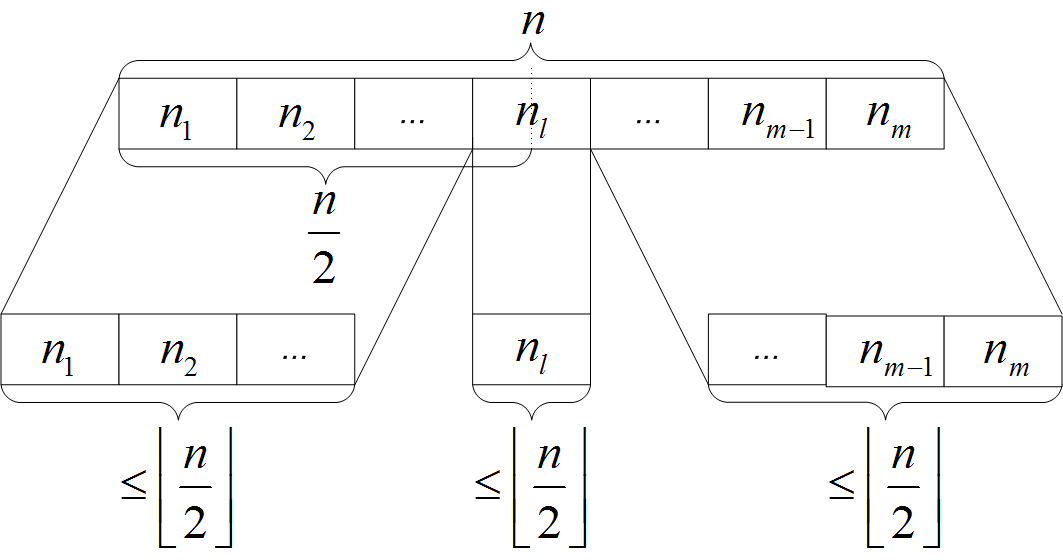
\includegraphics[scale=1.0]{images/three_division.png}
\caption{Разбиение множества деревьев $\{T_i\}$ на три группы, в каждой из которых суммарно не более $\left\lfloor\frac{n}{2}\right\rfloor$ вершин.}
\label{fig:three_division}
\end{figure}

Тогда неравенство (\ref{eq:psi_decomp_2}) преобразуется в:
\begin{equation}\label{eq:psi_decomp_3}
\begin{aligned}
\psi(\gF) &\le 2^k \sum_{i = 1}^{m} \psi(\gF_i) \\
&= 2^k \left( \sum_{i = 1}^{l-1} \psi(\gF_i) + \psi(\gF_l) + \sum_{i = l+1}^{m} \psi(\gF_i) \right) \\
&\le 2^k \left( \sum_{i = 1}^{l-1} \phi(n_i, k) + \phi(n_l, k) + \sum_{i = l+1}^{m} \phi(n_i, k) \right) \\
&\{\text{согласно (\ref{eq:phi_additive})} \} \\
&\le 2^k \left( \phi(\sum_{i = 1}^{l-1} n_i, k) + \phi(n_l, k) + \phi(\sum_{i = l+1}^{m} n_i, k) \right) \\
&\{\text{$\phi$ --- неубывает по $n$}\}\\
&\le 3 \cdot 2^k \phi(\left\lfloor\frac{n}{2}\right\rfloor, k) \text{.}
\end{aligned}
\end{equation}

Так как $\phi(1, k) = 2$, то согласно (\ref{eq:psi_decomp_3}), для функции $\phi$ справедлива следующая оценка:
\begin{equation}
\phi(n, k) \le 2 \cdot 2^{k \log_2{n}}3^{\log_2{n}} = 2n^{k + \log_2{3}}\text{,}
\end{equation}
что завершает доказательство леммы.
\end{proof}
\vspace{1cm}



Полученное неравенство дает верхнюю оценку размера множества $\gFc$. В результате проведения экспериментов было выяснено, что в задачах, встречающихся на практике, размер множества $\gFc$ в большинстве случаев не превышает $n^2$.

Для множества $\gFc$ выполнена следующая лемма.

\vspace{1cm}
\begin{lemma}\label{lemma:f_closure_tree}
Для произвольного множества классов $\gC$ выполнено $\forall T \in \nT(\gC), \gF \subseteq 2^{\gC}: \isPartSol(T, \gF) \Longrightarrow \isPartSol(T, \gFc)$.
\end{lemma}
\begin{proof}
Пусть утверждение леммы не верно. Тогда, согласно (\ref{eq:is_partial_solution}), $\exists~\gf':~T[\gf'] \notin \nT(\gf')$. Множество $\gf'$ не может быть пустым, потому как сужение дерева на пустое множество является деревом, и не может содержать только одну вершину, так как сужение дерева на множество из одной вершины также всегда является деревом. Следовательно, в множестве $\gf'$ содержится минимум две вершины.

В $T[\gf']$ не может быть циклов, так как их нет в $T$, и при сужении не добавляются новые ребра. Следовательно, $T[\gf']$ может не быть деревом только если оно не связно. Не нарушая общности, будем считать, что в $T[\gf']$ --- две компоненты связности. Пусть вершина $A$ лежит в первой компоненте, а $B$ --- во второй. По определению множества $\gFc$, $\gf'$ было получено пересечением некоторого количества множеств из $\gF$, то есть:
\begin{equation}
\gf' = \bigcap_{\gf \in \gF'} \gf \text{,}
\end{equation}
где $\gF' \subseteq \gF$. Значит, вершины $A$ и $B$ принадлежат всем множествам из $\gF'$. Так как по условию леммы $\forall \gf \in \gF': T[\gf] \in \nT(\gf)$, то если бы в $T$ между $A$ и $B$ существовал только один простой путь, то он принадлежал бы всем деревьям $T[\gf]$, где $\gf \in \gF'$, и, следовательно, все вершины этого простого пути принадлежали бы пересечению множеств из $\gF'$, и потому этот простой путь также принадлежал бы дереву $T[\gf']$, что противоречит предположению об отсутствии пути между вершинами $A$ и $B$ в $T[\gf']$. Следовательно, в $T$ существует несколько простых путей между $A$ и $B$. Но $T$ --- это дерево, и потому в нем существует единственный простой путь между вершинами $A$ и $B$. Полученное противоречие завершает доказательство леммы.
\end{proof}
\vspace{1cm}



Рассмотрим множество $\gFs$, определенное следующим образом:
\begin{equation}\label{eq:gfs_def}
\gFs = \gFc \cup \{\gCa\} \cup \bigcup_{C \in \gCa}\{\{C\}\} \setminus \emptyset \text{.}
\end{equation}

В силу того, что $T[\gCa] = T$, и сужение любого дерева на множество из одного элемента также является деревом, выполнено:
\begin{equation}\label{eq:gfs_tree}
\isPartSol(T, \gFc) \Longleftrightarrow \isPartSol(T, \gFs) \text{.}
\end{equation}

По построению также выполнено, что любое пересечение множеств из $\gFs$ содержится в $\gFs$. Тогда из (\ref{eq:is_sol_req_2}), (\ref{eq:gfs_tree}) и леммы \ref{lemma:f_closure_tree} следует:
\begin{equation}\label{eq:is_sol_req_3}
\forall T \in \nT^R(\gCa): \isSol(T. \gR) \Longrightarrow \isPartSol(T[\nT], \gFs) \text{,}
\end{equation}
то есть $\isPartSol(T[\nT], \gFs)$ является необходимым условием того, что дерево $T$ является решением задачи (\ref{eq:problem}).

Рассмотрим отношение $\subset$ на множестве $\gFs$. Это отношение является отношением частичного порядка, и поэтому для него можно построить диаграмму Хассе.

Диаграмма Хассе\footnote{англ. Hasse diagram.} --- графическое представление частично упорядоченного множества $(X, \le)$, в котором с каждым элементом $X$ сопоставляется точка плоскости таким образом, что меньшая точка всегда располагается ниже большей точки. Две точки $x$ и $y$ в диаграмме Хассе соединены тогда и только тогда, когда $x \le y$, и не существует такой точки $z$, что $x \le z \le y$.

Пусть диаграмма Хассе $\gH = (\gFs, \subset)$ для множества $\gFs$ построена. Каждой вершине $\gH$ соответствует множество из $\gFs$. Будем обозначать вершины $\gH$ также, как и элементы множества $\gFs$, то есть если $\gf \in \gFs$, то будем говорить, что $\gf$ является вершиной $\gH$. В силу (\ref{eq:is_sol_req_3}), если дерево $T$ является решением задачи (\ref{eq:problem}), то каждой вершине $\gf$ диаграммы Хассе $\gH$ соответствует поддерево $T[\gf]$ дерева $T$.

Диаграмму Хассе $\gH$ можно рассматривать как неориентированный граф. Будем обозначать множество ребер этого графа $\gH_E$.

Рассмотрим алгоритм построения дерева $T$ такого, что выполнено $\isPartSol(T, \gFs)$, представленный на рис. \ref{alg:build_tree}.

\begin{figure}[htb!]
\begin{algorithmic}[1]
\STATE $T_E = \emptyset$
\FORALL{$\gf \in \gFs$}
    \STATE $\gD \gets \{\gf' \in \gFs | \gf' \subset \gf \wedge \{\gf, \gf'\} \in \gH_E\}$
    \STATE $\gK \gets \gD$
    \WHILE{$\exists \gf_1, \gf_2 \in \gK: \gf_1 \cap \gf_2 \ne \emptyset$}
        \STATE $\gK \gets \gK \setminus \{\gf_1, \gf_2\} \cup \{\gf_1 \cup \gf_2\}$
    \ENDWHILE
    \STATE $t \gets any(\nT(\gK))$
    \FORALL{$\{\gf_1, \gf_2\} \in t_E$}
        \STATE $T_E \gets T_E \cup \{any(\gf_1), any(\gf_2)\}$
    \ENDFOR
\ENDFOR
\RETURN $T = (\gCa, T_E)$
\end{algorithmic}
\caption{Алгоритм построения дерева $T$ по множеству $\gFs$.}
\label{alg:build_tree}
\end{figure}

Представленный на рис. \ref{alg:build_tree} алгоритм использует функцию $any$, которая возвращает произвольный элемент данного множества. Для этого алгоритма справедлива следующая теорема.



\vspace{1cm}
\begin{theorem}\label{theorem:evil}
Если $\exists T' \in \nT(\gCa): \isPartSol(T', \gFs)$, то алгоритм, представленный на рис. \ref{alg:build_tree}, строит дерево $T \in \nT(\gCa): \isPartSol(T, \gFs)$ независимо от того, какие значения были возвращены функциями $any$.
\end{theorem}
\begin{proof}
Покажем, что в результате применения алгоритма будет выполнено $\forall \gf \in \gFs: T[\gf] \in \nT(\gf)$. Так как $\gCa \in \gFs$, то из этого будет следовать справедливость теоремы.

Будем рассматривать вершины диаграммы Хассе $\gH$ в порядке снизу вверх. Такой порядок просмотра гарантирует, что при рассмотрения очередного множества $\gf \in \gFs$, все множества $\gf' \in \gFs: \gf' \subset \gf$ будут уже рассмотрены. Пронумеруем элементы множества $\gFs$ в соответствии с этим порядком: $\gFs = \{\gf_1, \gf_2, \ldots, \gf_{|\gFs|}\}$. В этом случае будет справедливо
\begin{equation}\label{eq:seq_prop}
\gf_i \subset \gf_j \Longrightarrow i < j \text{.}
\end{equation}

Пусть
\begin{equation}\label{eq:induct}
\forall \gf_i: 1 \le i \le n - 1: T[\gf_i] \in \nT(\gf_i) \text{,}
\end{equation}
где $1 \le n \le |\gFs|$. Покажем, что в этом случае будет выполнено и $T[\gf_n] \in \nT(\gf_n)$.

В случае, если $\gf_n$ состоит из одной вершины, $T[\gf_n]$ является деревом.

Рассмотрим случай $|\gf_n| > 1$. В процессе выполнения алгоритма к $\gf_n$ было применено тело основного цикла. В результате было построено соответствующее $\gf_n$ множество $\gD$. Согласно определению множества $\gD$, в нем содержатся все вершины диаграммы Хассе $\gH$, находящиеся ниже $\gf_n$, и соединенные с $\gf_n$ ребром. Так как $|\gf_n| > 1$, то согласно (\ref{eq:gfs_def}), выполнено $\forall C \in \gf_n: \{C\} \in \gFs$, и потому множество $\gD$ не пусто.

Рассмотрим множество $\gK$, построение которого происходит в строках 4-7 алгоритма. По построению выполнено:
\begin{equation}\label{eq:gk_props}
\begin{aligned}
&\forall \gf'_1, \gf'_2 \in \gK: \gf'_1 \ne \gf'_2 \Longrightarrow \gf'_1 \cap \gf'_2 = \emptyset \\
&\gf_n = \bigcup_{\gf' \in \gK} \gf'
\end{aligned}
\end{equation}

В строках 8-11 над множеством $\gK$ строится произвольное дерево, и в соответствии со структурой этого дерева добавляются ребра к дереву $T$. Заметим, что если выполнено $\forall \gf' \in \gK: T[\gf'] \in \nT(\gf')$, то будет также выполнено и $T[\gf_n] \in \nT(\gf_n)$. Действительно, если над каждым из множеств из $\gK$ уже построено дерево, то в силу (\ref{eq:gk_props}), в результате добавления ребер в строках 8-11 алгоритма $T[\gf_n]$ будет связным графом с $\sum_{\gf' \in \gK} |\gf'|$ вершин и $\sum_{\gf' \in \gK} (|\gf'| - 1) + |\gK| - 1 = \sum_{\gf' \in \gK} |\gf'| - 1$ ребер, то есть деревом.

Покажем, что для всех $\gf' \in \gK$, $T[\gf']$ является деревом. Проведем доказательство для некоторого отдельного множества $\gf' \in \gK$. По построению, каждый элемент множества $\gK$ является объединением некоторого количества элементов множества $\gD$, то есть:
\begin{equation}\label{eq:gft_is_gc_gft_union}
\gf' = \bigcup_{\gf \in \gD} \gf \text{,}
\end{equation}
где $\gD \subseteq \gD$. Так как для всех $\gf \in \gD$ выполнено $\gf \subset \gf_n$, то в силу (\ref{eq:seq_prop}) и (\ref{eq:induct}), также выполнено:
\begin{equation}\label{eq:all_in_gc_are_trees}
\forall \gf \in \gD: T[\gf_i] \in \nT(\gf_i) \text{.}
\end{equation}

Из (\ref{eq:gft_is_gc_gft_union}) и (\ref{eq:all_in_gc_are_trees}) следует, что $\forall \gf \in \gD: T[\gf_i] \in \nT(\gf_i)$. То есть $T[\gf']$ является <<объединением>> некоторого количества деревьев, причем граф $T[\gf']$ связен. Покажем, что $T[\gf']$ --- дерево.

Пусть это не так. Так как граф $T[\gf']$ связен, и не является деревом, то в нем должен присутствовать один или несколько простых циклов, то есть циклов, в которых вершины и ребра не повторяются.

Пусть отношение $\subseteq$ на множестве неориентированных графов над некоторым множеством $X$ определено как $\forall G = (G_V, G_E), G' = (G'_V, G'_E) \in \nG(X): G \subseteq G' \Longleftrightarrow G_V \subseteq G'_V \wedge G_E \subseteq G'_E$, то есть $G$ является подграфом $G'$. Тогда зададим отношение $\subset$: $\forall G, G' \in \nG(X): G \subset G' \Longleftrightarrow G \subseteq G' \wedge G \ne G'$. Аналогично вводятся операции $\cup$ и $\cap$ над множеством $\nG(X)$.

Рассмотрим некоторый простой цикл $S \subseteq T[\gf']$. Тогда для любого $\gf \in \gD$ пересечение $S \cap T[\gf]$ пусто или состоит из одного или нескольких отрезков из $S$. Каждый такой отрезок может быть рассмотрен как простой путь в $S$, то есть путь, в котором вершины и ребра не повторяются. Пусть $\gS_{\gf}$ --- множество таких отрезков для $\gf$. По построению для этого множества выполнено:
\begin{equation}\label{eq:gs_for_gf_def}
\forall_{\gs \in \gS_{\gf}, \gs' \subseteq S \cap T[\gf]} \; \text{$\gs'$ --- отрезок} \Longrightarrow \gs \cap \gs' = \emptyset \vee \gs' \subseteq \gs
\end{equation}

Будем считать, что каждый отрезок из $\gS_{\gf}$ помечен множеством $\gf$. Пусть $\gS$ является объединением всех таких множеств $\gS_{\gf}$, то есть:
\begin{equation}
\gS = \bigcup_{\gf \in \gD} \gS_{\gf} \text{.}
\end{equation}

По построению для $\gS$ выполнено:
\begin{equation}
\bigcup_{\gs \in \gS} \gs = S
\end{equation}

Так как каждый отрезок из $\gS$ помечен множеством из $\gD$, то пусть функция $\cI$ для каждого отрезка возвращает соответствующее ему множество из $\gD$.

Заметим, что если $\exists \gs_i, \gs_j \in \gS: \cI(\gs_i) = \cI(\gs_j)$, то между некоторыми двумя вершинами отрезков $\gs_i$ и $\gs_j$ существует простой путь $\gp_{ij}$ в $T[\cI(\gs_i)]$. Соответствующий пример представлен на рис. \ref{fig:two_same_segment}. Этот путь не может целиком лежать в $S$, так как тогда было бы нарушено (\ref{eq:gs_for_gf_def}) --- пересечение $T[\cI(\gs_i)]$ с $S$ состояло бы из одного или нескольких отрезков, одним из которых являлся бы $\gs_i \cup \gp_{ij} \cup \gs_j$, и потому отрезки $\gs_i$ и $\gs_j$ не попали бы в множество $\gS_{\cI(\gs_i)}$.

\begin{figure}[htb!]
\centering
\begin{minipage}[t]{0.4\textwidth}
\centering
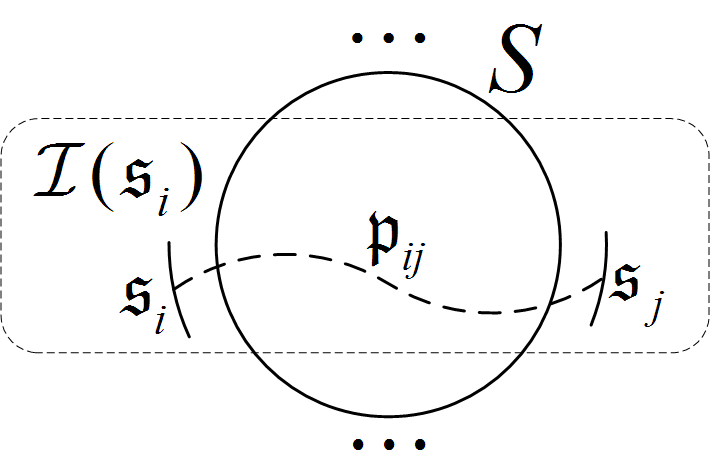
\includegraphics[scale=1.0]{images/two_same_segment.png}
\caption{Пример существования в простом цикле нескольких отрезков, которым соответствует одно и то же множество.}
\label{fig:two_same_segment}
\end{minipage}
\hspace{0.5cm}
\begin{minipage}[t]{0.4\textwidth}
\centering
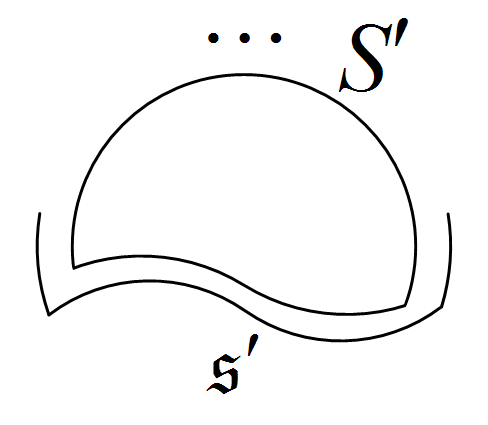
\includegraphics[scale=1.0]{images/two_same_segment_2.png}
\caption{Результат обработки случая, представленного на рис. \ref{fig:two_same_segment}.}
\label{fig:two_same_segment_2}
\end{minipage}
\end{figure}

Таким образом, между некоторыми двумя вершинами, лежащими на отрезках $\gs_i$ и $\gs_j$, существуют два простых пути --- один лежащий в $S$, другой --- лежащий в $\gp_{ij}$, причем ни один из этих простых путей не содержится в другом. Но тогда это означает, что в графе, построенном путем объединения этих двух простых путей, существует простой цикл. Обозначим этот цикл $S^{(1)}$. Пусть $\gs^{(1)} = (\gs_i \cup \gp_{ij} \cup \gs_j) \cap S^{(1)}$, тогда простой цикл $S^{(1)}$ можно покрыть множеством отрезков:
\begin{equation}\label{eq:gs_1_def}
\gS^{(1)} \subseteq \gS \cup \{\gs^{(1)}\} \setminus \{\gs_i, \gs_j\}
\end{equation}

Будем считать, что $\gS^{(1)}$ выбрано так, что все отрезки из $\gS^{(1)}$ имеют непустое пересечение с $S^{(1)}$. Так как в процессе построения структура цикла была изменена, то для некоторых отрезков из $\gS^{(1)}$ может больше не выполняться (\ref{eq:gs_for_gf_def}), примененное к циклу $S^{(1)}$, то есть не обязательно выполняется:
\begin{equation}\label{eq:gs_for_gf_def_2}
\forall_{\gs \in \gS^{(1)}, \gs' \subseteq S^{(1)} \cap T[\cI(\gs)]} \; \text{$\gs'$ --- отрезок} \Longrightarrow \gs \cap \gs' = \emptyset \vee \gs' \subseteq \gs
\end{equation}

Заменим каждый отрезок $\gs \in \gS^{(1)}$ на $\gs_+$ такой, что для $\gs_+$ выполняется (\ref{eq:gs_for_gf_def_2}), и при этом $\gs \cap \gs_+ \ne \emptyset$. Полученное таким образом новое множество отрезков обозначим $\gS^{(1)}_+$. Будем считать, что если в результате замены в $\gS^{(1)}_+$ были добавлены два равных отрезка, которым соответствует одно и то же множество из $\gD$, то такие отрезки представлены в множестве $\gS^{(1)}_+$ только один раз. Так как множество $\gS^{(1)}$ покрывало цикл $S^{(1)}$, то и построенное множество $\gS^{(1)}_+$ будет его покрывать.

Заметим, что в силу (\ref{eq:gs_1_def}), выполнено $|\gS^{(1)}| < |\gS|$, и потому также выполнено $|\gS^{(1)}_+| < |\gS|$. Так как количество отрезков в множестве $\gS$ конечно, то повторяя несколько раз приведенные выше рассуждения, на $k$-м шаге будет выполнено $\nexists \gs_i, \gs_j \in \gS^{(k)}_+: \cI(\gs_i) = \cI(\gs_j)$.

Выделим минимальное подмножество отрезков $\gS_{\min} \subseteq \gS^{(k)}_+$, покрывающих весь простой цикл $S^{(k)}$, то есть:
\begin{equation}\label{eq:gsmin_def}
\begin{aligned}
\bigcup_{\gs \in \gS_{\min}} \gs &= S^{(k)} \\
\forall \gs' \in \gS_{\min} \bigcup_{\gs \in \gS_{\min} \setminus \{\gs'\}} \gs &\ne S^{(k)}
\end{aligned}
\end{equation}

\begin{figure}[htb!]
\centering
\begin{minipage}[t]{0.4\textwidth}
\centering
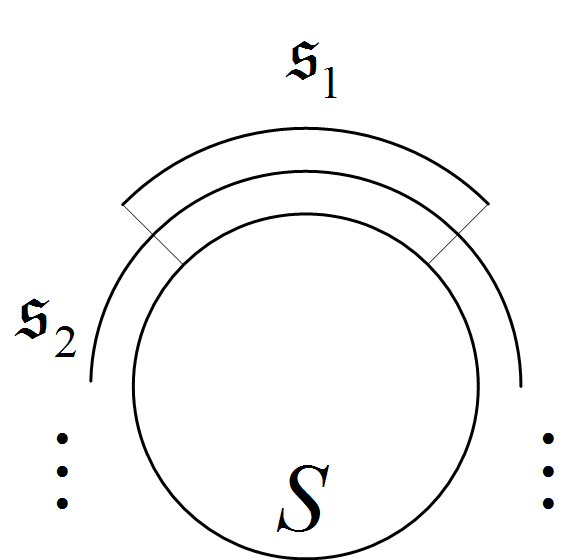
\includegraphics[scale=1.0]{images/two_segment.png}
\caption{Пример отрезка, лежащего целиком внутри другого отрезка.}
\label{fig:two_segments}
\end{minipage}
\hspace{0.5cm}
\begin{minipage}[t]{0.4\textwidth}
\centering
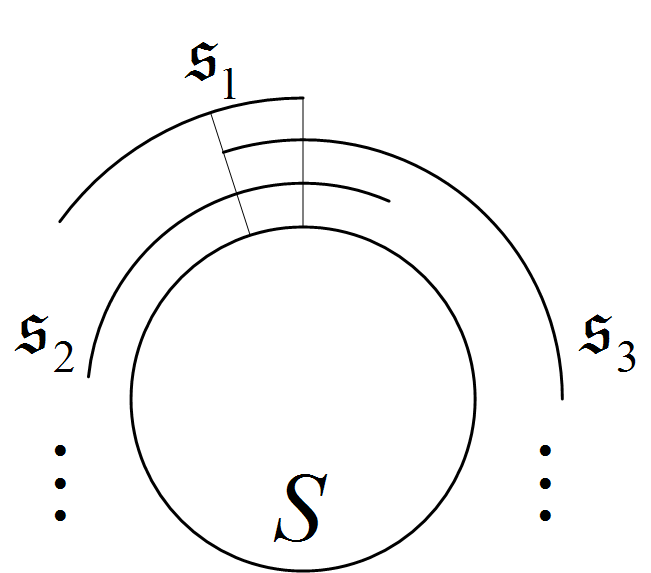
\includegraphics[scale=1.0]{images/three_segment.png}
\caption{Пример пересечения отрезков кратности три.}
\label{fig:three_segments}
\end{minipage}
\end{figure}

Для этого подмножества выполнено:
\begin{itemize}
\item В $\gS_{\min}$ нет отрезков, целиком лежащих внутри других. Если $\exists \gs_1, \gs_2 \in \gS_{\min}: \gs_1 \subseteq \gs_2$, то $\gS'_{\min} = \gS_{\min} \setminus \{\gs_1\}$ также покрывает весь простой цикл $S^{(k)}$, что противоречит определению множества $\gS_{\min}$. Пример для данного случая представлен на рис. \ref{fig:two_segments}.
\item Среди пересечений отрезков из $\gS_{\min}$ нет пересечений кратности три. На рис. \ref{fig:three_segments} представлен пример пересечения кратности три. Как видно, отрезок $\gs_1$ не может содержаться в $\gS_{\min}$, так как отрезки $\gs_2$ и $\gs_3$ и так покрывают соответствующие $\gs_1$ вершины и ребра. В общем случае, если существует пересечение кратности три, то среди отрезков, его образующих, существует отрезок $\gs_1$ такой, что $\gs_1 \subseteq \gs_2 \cup \gs_3$, где $\gs_2$ и $\gs_3$ --- два оставшихся отрезка в этом пересечении. Тогда $\gS'_{\min} = \gS_{\min} \setminus \{\gs_1\}$ также покрывает весь простой цикл $S^{(k)}$, что противоречит определению множества $\gS_{\min}$.
\end{itemize}

Таким образом, среди пересечений отрезков из $\gS_{\min}$ существуют только пересечения кратности два, и простой цикл $S^{(k)}$ можно представить как последовательность отрезков $S^{(k)} = (\gs_1, \ldots, \gs_n)$, в которой только соседние отрезки имеют непустое пересечение. Выбрав по точке на каждом пересечении соседних отрезков, получим последовательность точек $(C_1, \ldots, C_n)$ такую, что любые две соседние точки $C_i$ и $C_{i + 1}$ лежат в отрезке $\gs_i$, и потому лежат и в $\cI(\gs_i)$.

По условию теоремы, $\exists T' \in \nT(\gCa): \isPartSol(T', \gFs)$, то есть сужение дерева $T'$ на любое множество из $\gFs$ является деревом. Тогда сужение $T'$ на любое из множеств $\cI(\gs_i)$ также является деревом, и потому в каждом из таких деревьев существует единственный простой путь между соответствующими вершинами $C_i$ и $C_{i + 1}$. Обозначим этот простой путь $\gp_i$. По построению эти простые пути образуют цикл $S_{T'} = (\gp_1, \ldots, \gp_n)$. Так как $T'$ является деревом, то этот цикл не может быть простым, и каждая вершина из этого цикла принадлежит как минимум двум простым путям. Это означает, что в этом цикле существуют два простых пути $\gp_i$ и $\gp_{i+1}$, образующих <<поворот>>, как это изображено на рис. \ref{fig:tree_turn}.

\begin{figure}[htb!]
\centering
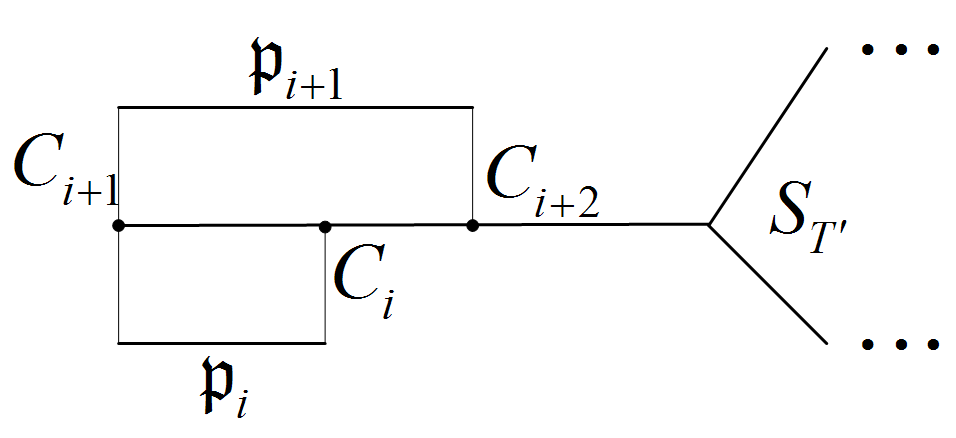
\includegraphics[scale=1.0]{images/tree_turn.png}
\caption{Пример <<поворота>>, образованного двумя простыми путями в цикле, не являющимся простым.}
\label{fig:tree_turn}
\end{figure}

Но тогда один из простых путей $\gp_i$ и $\gp_{i+1}$ содержится в другом. Не нарушая общности, будем считать, что $\gp_i$ содержится в $\gp_{i+1}$. Это означает, что $C_i$ содержится в $\gp_{i + 1}$, и так как по построению множество вершин простого пути $\gp_{i + 1}$ является подмножеством $\cI(\gs_{i + 1})$, то $C_i \in \cI(\gs_{i + 1})$.

Вернемся к дереву $T$. По построению для $\cI(\gs_{i + 1})$ выполнено $C_{i + 1}, C_{i + 2} \in \cI(\gs_{i + 1})$. $T[\cI(\gs_{i + 1})]$ является деревом, и поэтому в нем существует единственный простой путь из $C_i$ в $C_{i + 1}$, и единственный простой путь из $C_{i + 1}$ в $C_{i + 2}$. Эти простые пути должны принадлежать циклу $S^{(k)}$, и потому в силу (\ref{eq:gs_for_gf_def_2}) они также должны принадлежать отрезку $\gs_{i + 1}$. Но тогда среди отрезков из $\gS_{\min}$ существует пересечение кратности три --- $C_i \in \gs_{i + 1}$, $C_i \in \gs_{i}$, $C_i \in \gs_{i - 1}$, что противоречит определению множества $\gS_{\min}$. Следовательно, изначальное предположение о том, что в $T[\gf']$ существует цикл, неверно, и $T[\gf']$ является деревом. 

Полученное противоречие доказывает, что если выполнено (\ref{eq:induct}), то выполнено и $T[\gf_n] \in \nT(\gf_n)$. Тогда применение метода математической индукции для индукционного перехода (\ref{eq:induct}) и для базы индукции $n = 1$, дает, что (\ref{eq:induct}) верно для всех $1 \le n \le |\gFs|$, что завершает доказательство теоремы.
\end{proof}
\vspace{1cm}



Следствием доказанной теоремы является то, что любое решение задачи (\ref{eq:problem}) может быть получено с помощью алгоритма \ref{alg:build_tree}, а также то, что если в результате применение алгоритма \ref{alg:build_tree} не было построено дерево, то невозможно одновременно удовлетворить все ограничения вида $\cR_{\ref{stmt:fsets_2}}$, порожденные утверждениями \ref{stmt:fsets_2}. В этом случае путем автоматического анализа имеющейся информации затруднительно выяснить, какое из ограничений вида $\cR_{\ref{stmt:fsets_2}}$ следует удалить из множества $\gR$. Поэтому будем считать, что в этом случае удаление вызывающего конфликт ограничения выполняется вручную. Как было отмечено в комментарии к утверждению \ref{stmt:fsets_2}, такая ситуация маловероятна. В дальнейшем будем считать, что все ограничения, порожденные утверждением \ref{stmt:fsets_2}, выполнены. Для этого случая модифицируем алгоритм \ref{alg:build_tree} так, чтобы он строил только решения задачи (\ref{eq:relaxed_problem}).











\subsubsection{Алгоритм построения решения задачи восстановления одиночного наследования}\label{chapter:restore_single_inheritance}
Рассмотрим диаграмму Хассе $\gH$. Алгоритм \ref{alg:build_tree} для каждой вершины $\gf$ этой диаграммы строит множество $\gD$. Будем называть элементы этого множества дочерними вершинами для $\gf$ в диаграмме Хассе $\gH$. По диаграмме Хассе $\gH$ построим граф $\gG$, вершинами которого также являются множества $\gf \subset \gCa$, но разделенные на два типа --- $\any$ и $\fixed$. Алгоритм построения этого графа представлен на рис. \ref{alg:build_gg}. Этот алгоритм использует следующие функции:

{\centering
\begin{tabularx}{\textwidth}{rcX}
      \children & --- & возвращает множество дочерних вершин $\gD$ для данного множества $\gf$. Построение множества $\gD$ происходит также, как и в алгоритме \ref{alg:build_tree}; \\
 \textit{merge} & --- & возвращает множество $\gK$ для данного множества $\gD$. Построение множества $\gK$ происходит также, как и в алгоритме \ref{alg:build_tree}. \\
\end{tabularx}}

% \textit{\type} & --- & возвращает новую вершину, заданную множеством составляющих ее классов, и ее типом. \\
%Будем рассматривать вершины диаграммы Хассе $\gH$ в порядке снизу вверх. Такой порядок просмотра гарантирует, что при рассмотрения очередного множества $\gf \in \gFs$, все множества $\gf' \in \gFs: \gf' \subset \gf$ будут уже рассмотрены. Пронумеруем элементы множества $\gFs$ в соответствии с этим порядком: $\gFs = \{\gf_1, \gf_2, \ldots, \gf_{|\gFs|}\}$.

%Возвращаемые функциями \children~и \textit{merge} множества строятся также, как и в алгоритме \ref{alg:build_tree}.

\begin{figure}[htb!]
\begin{algorithmic}[1]
\STATE $\gG \gets (\emptyset, \emptyset)$
\FORALL{$\gf_1 \in \gFs$}
    \STATE $\gD \gets \children(\gf_1)$
    \STATE $\gK \gets \textit{merge}(\gD)$
    \STATE $\type(\gf_1) \gets \any$
    \STATE $\gG_V \gets \gG_V \cup \{\gf_1\}$
    \FORALL{$\gf_2 \in \gK$}
        \STATE $\gG_E \gets \gG_E \cup \{\{\gf_1, \gf_2\}\}$
        \IF{$\gf_2 \notin \gD$}
            \STATE \COMMENT{Это значит, что $\gf_2$ не является вершиной диаграммы Хассе $\gH$, и потому $\gf_2$ еще не было добавлено в $\gG_V$}
            \STATE $\type(\gf_2) \gets \fixed$
            \STATE $\gG_V \gets \gG_V \cup \{\gf_2\}$
            \FORALL{$\gf_3 \in \gD: \gf_3 \subseteq \gf_2$}
                \STATE $\gG_E \gets \gG_E \cup \{\{\gf_2, \gf_3\}\}$
            \ENDFOR
        \ENDIF
    \ENDFOR
\ENDFOR
\end{algorithmic}
\caption{Алгоритм построения графа $\gG$ по диаграмме Хассе $\gH$.}
\label{alg:build_gg}
\end{figure}

\begin{figure}[htb!]
\centering
\begin{minipage}[t]{0.4\textwidth}
\centering
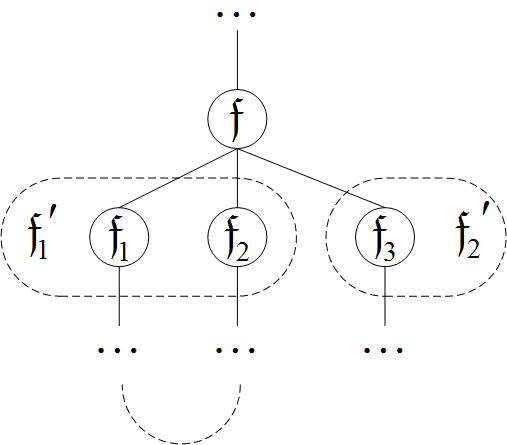
\includegraphics[scale=1.0]{images/gg_algo_class.png}
\caption{Пример части диаграммы Хассе, обрабатываемой алгоритмом \ref{alg:build_gg}.}
\label{fig:gg_algo_example}
\end{minipage}
\hspace{0.5cm}
\begin{minipage}[t]{0.4\textwidth}
\centering
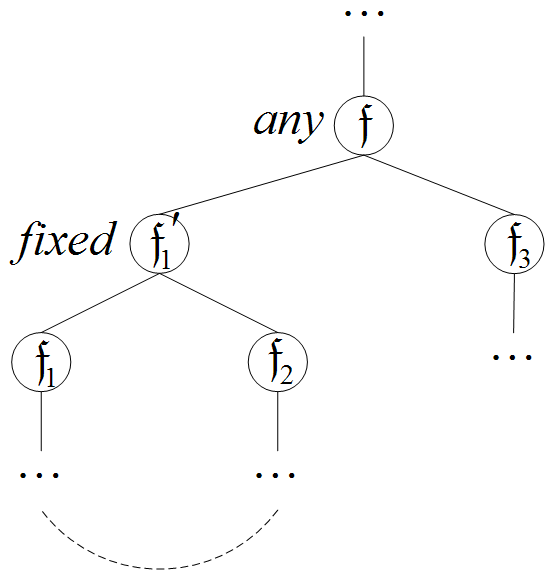
\includegraphics[scale=1.0]{images/gg_algo_class_2.png}
\caption{Результат обработки алгоритмом \ref{alg:build_gg} части диаграммы Хассе, представленной на рис. \ref{fig:gg_algo_example}.}
\label{fig:gg_algo_result}
\end{minipage}
\end{figure}

Пример работы алгоритма \ref{alg:build_gg} приведен на рис. \ref{fig:gg_algo_example} и рис. \ref{fig:gg_algo_result}. На рис. \ref{fig:gg_algo_example} представлена часть исходной диаграммы Хассе $\gH$, а на рис. \ref{fig:gg_algo_result} --- соответствующая ей часть графа $\gG$. Так как вершины $\gf_1$ и $\gf_2$ диаграммы Хассе $\gH$ лежат в одном множестве $\gf'_1 \in \gK$, то для них была добавлена $\fixed$-вершина $\gf'_1$. Для вершины же $\gf_3$ выполнено $\gf_3 = \gf'_2$, и потому $\gf'_2 \in \gD$, и для $\gf_3$ дополнительных $\fixed$-вершин добавлено не было.

По построению, граф $\gG$ является диаграммой Хассе для множества, подмножеством которого является $\gFs$, и потому на $\gG$ определен порядок расположения вершин на плоскости, и аналогично $\gH$ для каждой вершины определено множество дочерних вершин. Также по построению каждой $\any$-вершине в $\gG$ соответствует вершина в $\gH$, и наоборот. Тогда, согласно теореме \ref{theorem:evil}, выбирая для каждой $\any$-вершины дерево на множестве ее дочерних вершин, и добавляя после этого ребра к дереву $T \in \nT(\gCa)$ так, как в алгоритме \ref{alg:build_tree}, можно получить произвольное дерево, являющееся частичным решением задачи \ref{eq:problem}.

%Согласно утверждениям \ref{stmt:fsets_2}

С помощью графа $\gG$ построим полное решение задачи \ref{eq:relaxed_problem}.

%Для построения полного решения достаточно для каждого ребра построенного дерева $T$ определить направление наследование на этом ребре так, чтобы для каждой вершины дерева, то есть класса, существовал ровно один непосредственный базовый класс в этом дереве.

Заметим, что в графе $\gG$ нет циклов, проходящих только по $\any$-вершинам --- для существования цикла, проходящего через вершину $\gf$, и две ее дочерние вершины $\gf_1$ и $\gf_2$ необходимо, чтобы в $\gH$ существовал путь между вершинами $\gf_1$ и $\gf_2$. Но существование такого пути означает, что пересечение множеств $\gf_1$ и $\gf_2$ не пусто, и потому на этапе построения графа $\gG$ две эти вершины были отнесены к одному множеству $\gf'_1$, как это показано на рис. \ref{fig:gg_algo_example}. Следовательно, для этих вершин была добавлена $\fixed$-вершина, как это показано на рис. \ref{fig:gg_algo_result}, и потому они не могут являться дочерними для $\gf$. Это означает, что невозможно появление цикла, проходящего только по $\any$-вершинам, и содержащего вершины $\gf$, $\gf_1$ и $\gf_2$. Также для каждой $\any$-вершины $\gf$ графа $\gG$ выполнено:
\begin{equation}\label{eq:number_of_children}
|\children(\gf)| \le |\gCa| \text{,}
\end{equation}
то есть $\gf$ имеет не более $|\gCa|$ дочерних вершин. Если бы $\any$-вершина $\gf$ имела более $|\gCa|$ дочерних вершин, то пересечение некоторых двух из них было бы не пусто, что, как было только что доказано, невозможно.

Определим несколько функций. Пусть:

{\centering
\begin{tabularx}{\textwidth}{rcX}
    $\type$ & --- & возвращает тип данной вершины, то есть значение из множества $\{\any, \fixed\}$; \\
   $\class$ & --- & если для данной вершины $\gf$ выполнено $|\gf| = 1$, то есть $\gf = \{C\}$, то возвращает $C$, иначе возвращает $\emptyset$; \\
$\adjacent$ & --- & для данной вершины возвращает множество смежных с ней вершин в графе $\gG$; \\
 $\parents$ & --- & для данной вершины $\gf$ возвращает множество вершин, для которых $\gf$ является дочерней в $\gG$, то есть $\parents(\gf) = \adjacent(\gf) \setminus \children(\gf)$. По построению, если $\type(\gf) = \fixed$, то в этом множестве содержится ровно одна вершина. \\
\end{tabularx}}

Всевозможным парам вершин $(\gf_1, \gf_2)$ графа $\gG$ поставим в соответствие множества достижимых из $\gf_1$ по направлению на $\gf_2$ классов $\gC_{(\gf_1, \gf_2)}$. Если две вершины $\gf_1$ и $\gf_2$ инцидентны в графе $\gG$, то $\gC_{(\gf_1, \gf_2)}$ для них определяется согласно следующим правилам:
\begin{equation}\label{eq:cset_for_class}
\type(\gf_1) = \type(\gf_2) = \any \wedge \class(\gf_2) \ne \emptyset \Longrightarrow \gC_{(\gf_1, \gf_2)} = \class(\gf_2) \text{,}
\end{equation}

Иначе, если выполнено:
\begin{equation}\label{eq:cset_for_rest_cond}
\begin{aligned}
&\left( \type(\gf_1) = \type(\gf_2) = \any \right) \vee \\
&\left( \exists \{\gf'_1, \gf'_2\} = \{\gf_1, \gf_2\}: \type(\gf'_1) = \any \wedge \type(\gf'_2) = \fixed \wedge \parents(\gf'_2) = \{\gf'_1\} \right) \text{,}
\end{aligned}
\end{equation}
то есть $\gf_1$ и $\gf_2$ являются $\any$-вершинами, или одна из вершин $\gf_1$ и $\gf_2$ является $\fixed$-вершиной, а другая --- $\any$-вершиной, причем $\fixed$-вершина является дочерней для $\any$-вершины, то:
\begin{equation}\label{eq:cset_for_rest}
\gC_{(\gf_1, \gf_2)} = \bigcup_{\gf \in \adjacent(\gf_2) \setminus \gf_1} \gC_{(\gf_2, \gf)} \text{.}
\end{equation}

В случае, если не выполнено ни (\ref{eq:cset_for_class}), ни (\ref{eq:cset_for_rest_cond}), множество $\gC_{(\gf_1, \gf_2)}$ пусто.

Так как для двух вершин $\gf_1$ и $\gf_2$ таких, что $\gf_1$ является $\fixed$-вершиной, $\gf_2$ --- $\any$-вершиной, и $\gf_2$ является дочерней для $\gf_1$, множество $\gC_{(\gf_1, \gf_2)}$ пусто, то в силу отсутствия циклов в графе $\gG$, проходящих только по $\any$-вершинам, рекурсивное определение (\ref{eq:cset_for_rest}) множества $\gC_{(\gf_1, \gf_2)}$ корректно.

%Ребра графа $\gG$, инцидентные двум вершинам $\gf_1$ и $\gf_2$, для которых построенные с использованием правил (\ref{eq:cset_for_class})-(\ref{eq:cset_for_rest}) множества $\gC_{(\gf_1, \gf_2)}$ и $\gC_{(\gf_2, \gf_1)}$ не пусты, обозначим $\gE$.

Изменим множества $\gC_{(\gf_1, \gf_2)}$ для таких пар вершин, что $\gf_1$ является $\any$-вершиной, $\gf_2$ --- $\fixed$-вершиной, и между $\gf_2$ и $\gf_1$ в $\gG$ существует путь, содержащий только одну $\fixed$-вершину $\gf_2$, и такой, что каждая вершина в этом пути является дочерней для предыдущей. Это означает, что $\gf_2$ является <<первой>> $\fixed$-вершиной, находящейся над $\gf_1$, и связанной с ней. В этом случае будем считать, что
\begin{equation}
\gC_{(\gf_1, \gf_2)} = \gCa \setminus \left( \class(\gf_1) \cup \bigcup_{\gf \in \gCa} \gC_{(\gf_1, \gf)} \right)
\end{equation}
Тогда для каждой вершины $\gf$, по построению выполнено:
\begin{equation}\label{eq:gc_props}
\begin{aligned}
&\bigcup_{\gf' \in \gG_V} \gC_{(\gf, \gf')} = \gCa \setminus \class(\gf) \text{,} \\
&\forall_{\gf_1, \gf_2 \in \gG_V} \gC_{(\gf, \gf_1)} \cap \gC_{(\gf, \gf_2)} = \emptyset \text{.}
\end{aligned}
\end{equation}

Будем строить дерево, являющееся решением задачи (\ref{eq:relaxed_problem}) как дерево $T \in \nT(\gCa)$, для каждого ребра которого определено направление наследования. Для этого:
\begin{enumerate}
\item Для каждых двух дочерних вершин $\gf_1$ и $\gf_2$ каждой $\any$-вершины $\gf$ построим множество $\gN^{\gf}_{(\gf_1, \gf_2)}$ --- множество классов, которые должен унаследовать корень $T[\gf_1]$ в случае, если существует класс в $\gf_2$, являющийся предком этого корня, и множество $\gP^{\gf}_{(\gf_1, \gf_2)}$ --- множество классов, которые корень $T[\gf_1]$ не должен унаследовать в том же случае.
\item Для каждой $\any$-вершины $\gf$ построим корневое дерево $T_{\gf} \in \nT(\children(\gf))$ на множестве дочерних для нее вершин в $\gG$.
\end{enumerate}
Согласно определению, для множеств $\gN^{\gf}_{(\gf_1, \gf_2)}$ и $\gP^{\gf}_{(\gf_1, \gf_2)}$ выполнено:
\begin{equation}\label{eq:gn_gp_in_gc}
\gP^{\gf}_{(\gf_1, \gf_2)}, \gN^{\gf}_{(\gf_1, \gf_2)} \subseteq \gC_{(\gf_1, \gf_2)}
\end{equation}

Для построения корневых деревьев $T_{\gf}$ в каждой $\any$-вершине будем восстанавливать отношение $\lhd$ на множестве дочерних для нее вершин. Отношение $\lhd$ для вершины $\gf$ будем задавать множеством ограничений $\gR_{\gf}$. Будем считать, что в процессе восстановления это отношение задано ограничениями следующего вида:
\begin{equation}\label{eq:restriction_type}
\begin{aligned}
\cR &= B < D \text{,} &\text{или} \\
\cR &= B \lhd D \text{,} &\text{или} \\
\cR &= A \sim C \text{.} &~
\end{aligned}
\end{equation}
Ограничения вида $\cR = \neg (A \sim C)$ можно заменить двумя ограничениями $\cR_1 = A < C$ и $\cR_2 = A > C$ и рассматривать как ограничения вида (\ref{eq:restriction_type}).

Все ограничения из $\gR$, за исключением ограничений вида $\cR_{\ref{stmt:fsets_2}}$, полученных применением утверждения \ref{stmt:fsets_2}, представимы в виде \ref{eq:restriction_type}. Согласно предположению, высказанному в конце главы \ref{chapter:part_single_inher_rec}, все ограничения вида $\cR_{\ref{stmt:fsets_2}}$ выполнимы, и согласно теореме \ref{theorem:evil}, любое дерево, построенное с помощью алгоритма \ref{alg:build_tree}, удовлетворяет этим ограничениям. Тогда соблюдение ограничений вида $\cR_{\ref{stmt:fsets_2}}$ обеспечивается структурой построенного графа $\gG$ и выбранным способом построения корневого дерева, являющегося решением задачи (\ref{eq:relaxed_problem}).

Пусть $\gR_s \subseteq \gR$ --- множество всех ограничений из $\gR$, представимых в виде (\ref{eq:restriction_type}). Тогда в $\gR_s$ содержатся все ограничения из $\gR$, кроме ограничений вида $\cR_{\ref{stmt:fsets_2}}$. В начале главы \ref{chapter:full_sing_inhr_rec} было отмечено, что некоторые из ограничений из $\gR$ могут оказаться ложными, и вызвать конфликты в ходе восстановления иерархии. Будем строить иерархию, рассматривая ограничения из $\gR_s$ в порядке увеличения вероятности получения конфликта. Ограничения вида $\cR_{\ref{stmt:destructors}}$, определенные в утверждении \ref{stmt:destructors}, всегда выполняются, и являются наиболее информативными. В результате проведения экспериментов было выяснено, что во многих случаях только ограничений вида $\cR_{\ref{stmt:destructors}}$ и $\cR_{\ref{stmt:fsets_2}}$ достаточно, чтобы полностью восстановить иерархию классов. Поэтому будем рассматривать ограничения начиная с ограничений вида $\cR_{\ref{stmt:destructors}}$. В случае, если на очередном шаге обнаружится конфликт в структуре построенных множеств, в результате чего построение корневого дерева, являющегося решением, станет невозможным, будем возвращаться к предыдущему шагу, и продолжить обработку, добавив ограничение, вызвавшее конфликт, в изначально пустое множество конфликтных ограничений $\gR_{\times}$. Тогда после завершения обработки всех ограничений из $\gR_s$, множество ограничений $\gR \setminus \gR_{\times}$ будет соответствовать множеству ограничений $\gR'$ из определения задачи (\ref{eq:relaxed_problem}).


\begin{figure}[htb!]
\begin{algorithmic}[1]
\STATE \textbf{let} $\cR \in \gR_s, A, C \in \gCa: A \ne C \wedge \cR = A \sim C$
\STATE \textbf{let} $\gf_1: \class(\gf_1) = \{C\}$
\WHILE{$\class(\gf_1) \ne \{A\}$}
    \STATE \COMMENT{$\gf_2$ существует и единственно в силу (\ref{eq:gc_props})}
    \STATE \textbf{let} $\gf_2 \in \adjacent(\gf_1): A \in \gC_{(\gf_1, \gf_2)}$
    \IF{$\type(\gf_2) = \any \wedge \gf_1 \in \children(\gf_2) \wedge \exists \gf_3 \in \children(\gf_2): B \in \gC_{(\gf_2, \gf_3)}$}
%        \IF{$(\gf_1 \rhd \gf_3) \in \gR_{\gf_2}$}
%            \STATE $\gR_s \gets \gR_s \cup \{A \rhd C\}$
%        \ELSIF{$(\gf_3 \rhd \gf_1) \in \gR_{\gf_2}$}
%            \STATE $\gR_s \gets \gR_s \cup \{C \rhd A\}$
%        \ENDIF
%        \STATE $\gR_{\gf_2} \gets \gR_{\gf_2} \cup \{\gf_1 \sim \gf_3\}$
        \STATE $\gN^{\gf_2}_{(\gf_1, \gf_3)} \gets \gN^{\gf_2}_{(\gf_1, \gf_3)} \cup \{C\}$
        \STATE $\gN^{\gf_2}_{(\gf_3, \gf_1)} \gets \gN^{\gf_2}_{(\gf_3, \gf_1)} \cup \{A\}$
    \ELSIF{$\type(\gf_2) = \fixed \wedge \gf_2 \in \children(\gf_1)$}
        \STATE \textbf{break}
    \ENDIF
    \STATE $\gf_1 \gets \gf_2$
\ENDWHILE
\end{algorithmic}
\caption{Алгоритм обработки ограничения вида  $A \sim C$.}
\label{alg:process_sim}
\end{figure}

\begin{figure}[htb!]
\begin{algorithmic}[1]
\STATE \textbf{let} $\cR \in \gR_s, B, D \in \gCa: B \ne C \wedge \cR = B < D$
\STATE \textbf{let} $\gf_1: \class(\gf_1) = \{D\}$
\WHILE{$\class(\gf_1) \ne \{B\}$}
    \STATE \COMMENT{$\gf_2$ существует и единственно в силу (\ref{eq:gc_props})}
    \STATE \textbf{let} $\gf_2 \in \adjacent(\gf_1): B \in \gC_{(\gf_1, \gf_2)}$
    \IF{$\type(\gf_2) = \any \wedge \gf_1 \in \children(\gf_2) \wedge \exists \gf_3 \in \children(\gf_2): B \in \gC_{(\gf_2, \gf_3)}$}
        \STATE $\gN^{\gf_2}_{(\gf_1, \gf_3)} \gets \gN^{\gf_2}_{(\gf_1, \gf_3)} \cup \{B\}$
        \STATE $\gP^{\gf_2}_{(\gf_3, \gf_1)} \gets \gP^{\gf_2}_{(\gf_3, \gf_1)} \cup \{D\}$
    \ELSIF{$\type(\gf_2) = \fixed \wedge \gf_2 \in \children(\gf_1)$}
        \STATE \textbf{break}
    \ENDIF
    \STATE $\gf_1 \gets \gf_2$
\ENDWHILE
\end{algorithmic}
\caption{Алгоритм обработки ограничения вида $B < D$.}
\label{alg:process_less}
\end{figure}

\if 0
\begin{figure}[htb!]
\begin{algorithmic}[1]
\STATE \textbf{let} $\cR \in \gR_s: \cR = B \lhd D$
\STATE \textbf{let} $\gf_1: \class(\gf_1) = \{D\}$
\WHILE{$\class(\gf_1) \ne \{B\}$}
    \STATE \COMMENT{$\gf_2$ существует и единственно в силу (\ref{eq:gc_props})}
    \STATE \textbf{let} $\gf_2 \in \adjacent(\gf_1): B \in \gC_{(\gf_1, \gf_2)}$
    \IF{$\type(\gf_2) = \any \wedge \gf_1 \in \children(\gf_2) \wedge \exists \gf_3 \in \children(\gf_2): B \in \gC_{(\gf_2, \gf_3)}$}
        \STATE $\gR_{\gf_2} \gets \gR_{\gf_2} \cup \{\gf_1 \rhd \gf_3\}$
        \STATE $\gN^{\gf_2}_{(\gf_1, \gf_3)} \gets \gN^{\gf_2}_{(\gf_1, \gf_3)} \cup \{B\}$
    \ELSIF{$\type(\gf_2) = \fixed \wedge \gf_2 \in \children(\gf_1)$}
        \STATE \textbf{break}
    \ENDIF
    \STATE $\gf_1 \gets \gf_2$
\ENDWHILE
\end{algorithmic}
\caption{Алгоритм обработки ограничения вида $B \lhd D$.}
\label{alg:process_lhd}
\end{figure}
\fi

Будем считать, что изначально множества ограничений $\gR_{\gf}$, а также множества $\gN^{\gf}_{(\gf_1, \gf_2)}$ и $\gP^{\gf}_{(\gf_1, \gf_2)}$ пусты. Сначала рассмотрим все ограничения $\cR_{\ref{stmt:destructors}}$, затем --- все прочие ограничения вида $B \lhd D$. Так как отношение $\lhd$ можно выразить через отношения $<$ и $\sim$, то приведем алгоритмы модификации множеств $\gN^{\gf}_{(\gf_1, \gf_2)}$, $\gP^{\gf}_{(\gf_1, \gf_2)}$ и $\gR_{\gf}$ только для ограничений вида $B < D$ и $A \sim C$. Алгоритм отработки отдельного ограничения вида $A \sim C$ представлен на рис. \ref{alg:process_sim}, а ограничения вида $B < D$ --- на рис. \ref{alg:process_less}.

%Алгоритм модификации множеств $\gN^{\gf}_{(\gf_1, \gf_2)}$, $\gP^{\gf}_{(\gf_1, \gf_2)}$ и $\gR_{\gf}$ для отдельного ограничения такого вида представлен на рис. \ref{alg:process_lhd}.

После работы этих алгоритмов из измененных множеств $\gN^{\gf}_{(\gf_2, \gf_1)}$ и $\gP^{\gf}_{(\gf_1, \gf_2)}$ можно извлечь дополнительную информацию об ограничениях из $\gR_{\gf}$ с использованием правил поддержания непротиворечивости для множеств $\gR_{\gf}$. Из определения множеств $\gN^{\gf}_{(\gf_1, \gf_2)}$ и отношения $\sim$ следует:
\begin{equation}\label{eq:gf_consistency_1}
\begin{aligned}
&\forall \gf \in \gG_V: \type(\gf) = \any, \gf_1, \gf_2 \in \children(\gf): \gN^{\gf}_{(\gf_1, \gf_2)} \ne \emptyset \wedge \gN^{\gf}_{(\gf_2, \gf_1)} \ne \emptyset \\
&\quad \Longrightarrow (\gf_1 \sim \gf_2) \in \gR_{\gf}
\end{aligned}
\end{equation}

Множества $\gP^{\gf}_{(\gf_1, \gf_2)}$ и $\gN^{\gf}_{(\gf_1, \gf_2)}$ не должны конфликтовать, то есть должно быть выполнено:
\begin{equation}\label{eq:gf_consistency_2}
\begin{aligned}
&\forall \gf \in \gG_V: \type(\gf) = \any, \gf_1, \gf_2 \in \children(\gf): \gP^{\gf}_{(\gf_1, \gf_2)} \cap \gN^{\gf}_{(\gf_1, \gf_2)} \ne \emptyset \\
&\quad \Longrightarrow (\gf_1 < \gf_2) \in \gR_{\gf}
\end{aligned}
\end{equation}

Отношение $\lhd$ транзитивно, и потому выполнено:
\begin{equation}\label{eq:gf_consistency_3}
\begin{aligned}
&\exists \gf \in \gG_V: \type(\gf) = \any, \gf_1, \gf_2, \gf_3 \in \children(\gf): \{\gf_1 \rhd \gf_2, \gf_2 \rhd \gf_3\} \subseteq \gR_{\gf} \\
&\quad \Longrightarrow (\gf_1 \rhd \gf_3) \in \gR_{\gf} %\wedge \gN^{\gf}_{(\gf_2, \gf_3)} \subseteq \gN^{\gf}_{(\gf_1, \gf_3)}
\end{aligned}
\end{equation}

После применения правил поддержания непротиворечивости (\ref{eq:gf_consistency_1}), (\ref{eq:gf_consistency_2}) и (\ref{eq:gf_consistency_3}) в множества $\gR_{\gf}$ могут быть добавлены новые ограничения. Для элементов этих множеств используются следующие правила поддержания непротиворечивости:
\begin{equation}\label{eq:consistency_gr}
\begin{aligned}
b \lhd d &\Longleftrightarrow b < d \wedge b \sim d \\
b \lhd c \wedge c \lhd d &\Longrightarrow b \lhd d \\
d_1 \sim d_2, \ldots, d_{n - 1} \sim d_n, d_n \sim d_1\} &\Longrightarrow \forall a, c \in \{d_1, \ldots, d_n\}: a \sim c
\end{aligned}
\end{equation}
Эти правила опираются на свойства отношений $<$, $\lhd$ и $\sim$, а также на то, что эти отношения должны задавать деревья на множествах $\children(\gf)$. Также во множествах $\gR_{\gf}$ не должно существовать конфликтов, то есть не должно быть выполнено:
\begin{equation}\label{eq:consistency_conflict_1}
b \sim d \wedge b > d \wedge b < d
\end{equation}

Из измененных множеств $\gR_{\gf}$ может быть извлечена дополнительная информация об отношении наследования на множестве $\gCa$ с использованием правил поддержания непротиворечивости для множества $\gCa$. По одному ребру в дереве наследования не может быть унаследовано два класса, не связанных наследованием, и потому выполнено:
\begin{equation}\label{eq:gca_consistency_1}
\begin{aligned}
&\exists \gf \in \gG_V: \type(\gf) = \any, \gf_1, \gf_2 \in \children(\gf): \{\gf_1 \rhd \gf_2\} \subseteq \gR_{\gf}, A, C \in \gN^{\gf}_{(\gf_1, \gf_2)}: A \ne C \\
&\quad \Longrightarrow \text{~выполнено~} A \sim C
\end{aligned}
\end{equation}

В силу того, что в $\gG$ не существует цикла, проходящего только по $\any$-вершинам, выполнено:
\begin{equation}\label{eq:gca_consistency_2}
\begin{aligned}
&\exists \gf \in \gG_V: \type(\gf) = \any, \gf_1, \gf_2 \in \children(\gf): \{\gf_1 \rhd \gf_2\} \subseteq \gR_{\gf}, B \in \gN^{\gf}_{(\gf_1, \gf_2)} \\
&\quad \Longrightarrow \forall D \in \gC_{(\gf, \gf_1)}: \text{~выполнено~} D \rhd B
\end{aligned}
\end{equation}

\begin{equation}\label{eq:gca_consistency_3}
\begin{aligned}
&\exists \gf \in \gG_V: \type(\gf) = \any, \gf_1, \gf_2 \in \children(\gf): \{\gf_1 \rhd \gf_2\} \subseteq \gR_{\gf}, B \in \gN^{\gf}_{(\gf_1, \gf_2)} \\
&\quad \Longrightarrow \forall D \in \gP_{(\gf_1, \gf_2)}: \text{~выполнено~} D > B
\end{aligned}
\end{equation}

Таким образом, применение алгоритмов \ref{alg:process_sim} и \ref{alg:process_less} добавляет новые элементы в множества $\gN^{\gf}_{(\gf_2, \gf_1)}$ и $\gP^{\gf}_{(\gf_1, \gf_2)}$, применение правил поддержания непротиворечивости (\ref{eq:gf_consistency_1}), (\ref{eq:gf_consistency_2}) и (\ref{eq:gf_consistency_3}) на основе добавленных элементов добавляет ограничения в множества $\gR_{\gf}$, применение правил (\ref{eq:consistency_gr}) также добавляет новые ограничения в множества $\gR_{\gf}$, а применение правил поддержания непротиворечивости (\ref{eq:gca_consistency_1}) и (\ref{eq:gca_consistency_3}) добавляет новые ограничения на классы из $\gCa$, к которым снова можно применить алгоритмы \ref{alg:process_sim} и \ref{alg:process_less}. Так как все рассматриваемые множества конечны, то такой цикл применения алгоритмов \ref{alg:process_sim} и \ref{alg:process_less} и правил поддержания непротиворечивости (\ref{eq:gf_consistency_1}), (\ref{eq:gf_consistency_2}), (\ref{eq:gf_consistency_3}), (\ref{eq:consistency_gr}), (\ref{eq:gca_consistency_1}) и (\ref{eq:gca_consistency_3}) не может быть бесконечен. Этот цикл необходимо применить к каждому из ограничений из $\gR_s$.

Если в результате применения цикла к очередному ограничению $\cR$ из множества $\gR_s$ было нарушено (\ref{eq:consistency_conflict_1}) в одном из множеств $\gR_{\gf}$, или выяснилось, что не существует корневого дерева $T_{\gf} \in \nT^R(\children(\gf))$, удовлетворяющего ограничениям $\gR_{\gf}$, или (\ref{eq:consistency_conflict_1}) было нарушено для восстанавливаемого отношения наследования на множестве $\gCa$, то следует вернуться к предыдущему шагу, добавив ограничение $\cR$ в множество конфликтных ограничений $\gR_{\times}$.

%Количество ограничений в множестве $\gR_s$ конечно, и потому алгоритм завершится.

%Также в силу определения множеств $\gN^{\gf}_{(\gf_1, \gf_2)}$ должно быть выполнено:
%\begin{equation}\label{eq:consistency_4}
%\begin{aligned}
%&\exists \gf \in \gG_V: \type(\gf) = \any, \gf_1, \gf_2 \in \children(\gf), A \in \gN^{\gf}_{(\gf_1, \gf_2)}, C \in \gN^{\gf}_{(\gf_2, \gf_1)}: A \ne C \\
%&\quad \Longrightarrow \text{~выполнено~} A \sim C
%\end{aligned}
%\end{equation}

%Существование решения также требует:
%\begin{equation}\label{eq:consistency_6}
%\begin{aligned}
%&\exists \gf \in \gG_V: \type(\gf) = \any, \gf_1, \gf_2 \in \children(\gf): (\gf_1 \rhd \gf_2) \in \gR_{\gf}, B \in \gN^{\gf}_{(\gf_1, \gf_2)}, C \in \gP^{\gf_2}_{(\gf_3, \gf_1)} \\
%&\quad \Longrightarrow \text{~выполнено~} B < C
%\end{aligned}
%\end{equation}

%Если после обработки очередного ограничения возникает конфликт в (\ref{eq:consistency_conflict_1}), то следует вернуться к предыдущему шагу, и продолжить обработку прочих ограничений. Обработав все ограничения $B \lhd D$, перейдем к ограничениям $\cR = A \sim C$. Алгоритм обработки отдельного ограничения такого вида представлен на рис. \ref{alg:process_sim}.

%После работы этого алгоритма в множество $\gR_s$ могли быть добавлены новые ограничения вида $B \lhd D$. Их следует обработать в первую очередь. На следующем шаге следует обработать ограничения $B < D$. Алгоритм обработки ограничений такого вида представлен на рис. \ref{alg:process_less}.

%Этот алгоритм модифицирует множества $\gP^{\gf_2}_{(\gf_3, \gf_1)}$, для которых также должны быть выполнены правила консистентности. В силу транзитивности $\lhd$ должно быть выполнено:
%\begin{equation}\label{eq:consistency_5}
%\begin{aligned}
%&\exists \gf \in \gG_V: \type(\gf) = \any, \gf_1, \gf_2, \gf_3 \in \children(\gf): \{\gf_1 \rhd \gf_2, \gf_2 \rhd \gf_3\} \subseteq \gR_{\gf} \\
%&\quad \Longrightarrow \gP^{\gf}_{(\gf_1, \gf_3)} \subseteq \gP^{\gf}_{(\gf_2, \gf_3)}
%\end{aligned}
%\end{equation}

%Для множеств ограничений $\gR_{\gf}$ также должно использоваться правило поддержания консистентности (\ref{eq:consistency_gr}) и не должно существовать конфликтов вида (\ref{eq:consistency_conflict_1}), а также на каждом шаге должно быть возможно построить корневое дерево $T_{\gf} \in \nT^R(\children(\gf))$, удовлетворяющее ограничениям $\gR_{\gf}$. Если после обработки очередного ограничения возникает конфликт в (\ref{eq:consistency_conflict_1}), то следует вернуться к предыдущему шагу, и продолжить обработку прочих ограничений.

Обработав все ограничения, построим дерево $T$. Для этого для каждой $\any$-вершины $\gf$ построим корневое дерево $T_{\gf} \in \nT^R(\children(\gf))$ на множестве дочерних для нее вершин в $\gG$. По построению такое дерево существует. Будем рассматривать $\any$-вершины из $\gG$ в порядке снизу вверх и строить для них соответствующие деревья $T[\gf]$. Пусть $\gf$ --- очередная такая вершина, и для всех ее дочерних вершин соответствующие деревья уже построены, то есть $\forall \gf' \in \children(\gf): T[\gf'] \in \nT^R(\gf')$. Будем рассматривать такие деревья как ориентированные графы, в которых все дуги имеют направление от листьев к корню дерева. Для каждой дуги $(\gf_1, \gf_2)$ из $T_{\gf}$ добавим в $T$ дугу, соединяющую корень $T[\gf_1]$, и вершину из $\gf_2$ такую, что по дугам достижимы все вершины из $\gN^{\gf}_{(\gf_1, \gf_2)}$, и не достижимы вершины из $\gP^{\gf_2}_{(\gf_3, \gf_1)}$. Существование такой вершины следует из выполнения (\ref{eq:gca_consistency_3}). Добавив все такие дуги, выберем корень дерева $T[\gf_r]$ корнем построенного дерева $T[\gf]$, где $\gf_r$ --- корень $T_{\gf}$. Так как такое построение полностью соответствует описанному в алгоритме \ref{alg:build_tree}, то согласно теореме \ref{theorem:evil}, для построенного корневого дерева $T$ выполнены все ограничения, порожденные утверждением \ref{stmt:fsets_2}. По построению для этого дерева также выполнено множество ограничений $\gR \setminus \gR_{\times}$, и потому построенное дерево является решением задачи \ref{eq:relaxed_problem}.


Оценим сложность представленного алгоритма. Пусть $n$ --- количество классов в множестве $\gCa$. Как было отмечено в главе \ref{chapter:part_single_inher_rec}, в задачах, встречающихся на практике, размер множества $\gFc$ в большинстве случаев не превышает $n^2$. Пусть $N$ --- количество $\any$-вершин в графе $\gG$. Так как каждой $\any$-вершине графа $\gG$ соответствует элемент множества $\gFs$, то согласно (\ref{eq:gfs_def}), можно считать, что $N = O(n^2)$. Тогда в силу (\ref{eq:gc_props}), суммарный размер множеств $\gC_{(\gf_1, \gf_2)}$ не превосходит $nN$.

Дочерними вершинами $\any$-вершин могут быть другие $\any$-вершины, и $\fixed$-вершины. Так как в $\gG$ нет циклов, проходящих целиком по $\any$-вершинам, то количество ребер, соединяющих $\any$-вершины, не превосходит $N$. По построению графа $\gG$, у каждой $\fixed$-вершины есть дочерние вершины, причем дочерними вершинами $\fixed$-вершины могут быть только $\any$-вершины. Следовательно, в графе $\gG$ не более $N$ $\fixed$-вершин. Это в частности означает, что:
\begin{equation}\label{eq:vertices_in_ggv}
|\gG_V| \le 2N \text{.}
\end{equation}

Так как предком каждой $\fixed$-вершины является единственная $\any$-вершина, то суммарное количество дочерних вершин всех $\any$-вершин не превосходит $2N$, то есть:
\begin{equation}\label{eq:sum_children}
\sum_{\gf \in \gG_V: \type(\gf) = \any} |\children(\gf)| \le 2N \text{.}
\end{equation}

Тогда из (\ref{eq:vertices_in_ggv}) следует, что суммарный размер всех множеств, соответствующих вершинам графа $\gG$, не превосходит $2nN$. Из (\ref{eq:number_of_children}) и (\ref{eq:sum_children}) также следует, что суммарное количество ограничений в множествах $\gR_{\gf}$ не превосходит $6nN$. Также из (\ref{eq:gn_gp_in_gc}), (\ref{eq:gc_props}) и (\ref{eq:sum_children}) следует, что суммарный размер всех множеств $\gN^{\gf}_{(\gf_1, \gf_2)}$ и $\gP^{\gf}_{(\gf_1, \gf_2)}$ не превосходит $4Nn$. Число же различных ограничений на множестве $\gCa$ не превосходит $3n^2$.

Это означает, что затраты памяти предложенного алгоритма составляют $O(nN) = O(n^3)$. Оценим вычислительные затраты предложенного алгоритма. Проверка выполнения условий (\ref{eq:gf_consistency_1})-(\ref{eq:gca_consistency_3}) производится только в случае, если множество, для которого производится проверка, было изменено. В результате анализа проверок (\ref{eq:gf_consistency_1})-(\ref{eq:gca_consistency_3}) было выяснено, что для выполнения каждой их них требуется не более $O(n^2)$ операций. Так как в процессе работы алгоритма элементы только добавляются в множества $\gN^{\gf}_{(\gf_1, \gf_2)}$, $\gP^{\gf}_{(\gf_1, \gf_2)}$, $\gR_{\gf}$, и множество ограничений над $\gCa$, то проверки (\ref{eq:gf_consistency_1})-(\ref{eq:gca_consistency_3}) будут применены не более одного раза к каждому из элементов этих множеств. Следовательно, суммарная сложность предложенного алгоритма составляет $O(n^5)$.

Не смотря на высокую сложность, предложенный алгоритм применим для большинства возникающих на практике задач, связанных с восстановлением иерархий классов при отсутствии информации о типах времени выполнения. Это объясняется тем, что деревья наследования, состоящие более чем из 100 классов, встречаются в крупных библиотеках, таких как Qt \cite{qt} или MFC \cite{mfc}, которые в большинстве случаев используют ту или иную форму информации о типах времени выполнения, и поэтому для таких деревьев наследования применение предложенного алгоритма не требуется.



\subsection{Восстановление множественного наследования}
Как было сказано в главе \ref{chapter:multiple_inheritance}, так как большинство иерархий классов используют виртуальные деструкторы, то путем анализа деструкторов в большинстве случаев можно выявить использование множественного наследования и определить, какие таблицы виртуальных функций принадлежат одному и тому же классу. В главе \ref{chapter:restore_single_inheritance} был описан алгоритм восстановления отношения одиночного наследования на множестве таблиц виртуальных функций.

Результатом последовательного применения описанного в главе \ref{chapter:restore_single_inheritance} алгоритма  восстановления одиночного наследования на множестве таблиц виртуальных функций является одно или несколько деревьев наследования $T_1, \ldots, T_n$. Будем предполагать, что деревья наследования из $T_1, \ldots, T_n$ восстановлены корректно в смысле, определенном в главе \ref{chapter:problem}. Результатом анализа деструкторов на предмет использования множественного наследования является набор множеств таблиц виртуальных функций $\gv_1, \ldots, \gv_m$ такой, что все таблицы виртуальных функций, принадлежащие одному множеству, принадлежат одному классу. Тогда, каждое из множеств $\gv_i$ задает отдельный класс, использующий множественное наследование. Объединив для каждого из множеств $\gv_1, \ldots, \gv_m$ соответствующие вершины в деревьях $T_1, \ldots, T_n$, можно получить иерархию, учитывающую множественное наследование. При этом следует учитывать, что, вообще говоря, два множества $\gv_i$ и $\gv_j$ могут иметь непустое пересечение --- это будет означать, что классы, соответствующие $\gv_i$ и $\gv_j$, используют один и тот же деструктор, и разделяют некоторые из таблиц виртуальных функций. Тогда исходя из предположения о том, что деревья наследования $T_1, \ldots, T_n$ были восстановлены корректно, согласно правилам наследования Си++ \cite{cpp03}, отношение непосредственного наследования между таблицами виртуальных функций из $(\gv_i \cup \gv_j) \setminus (\gv_i \cap \gv_j)$ задает отношение непосредственного наследования между классами, соответствующими $\gv_i$ и $\gv_j$. Следовательно, можно заменить в соответствии с этим отношением непосредственного наследования каждую из вершин в деревьях $T_1, \ldots, T_n$, соответствующую таблицам виртуальных функций из $\gv_i \cap \gv_j$, на две, одна из которых будет соответствовать множеству $\gv_i$, а другая --- $\gv_j$, после чего произвести объединение вершин деревьев $T_1, \ldots, T_n$ также, как и в случае отсутствия пересечений между $\gv_i$ и $\gv_j$. Аналогично рассматривается случай существования более двух множеств из $\gv_1, \ldots, \gv_m$, имеющих непустое пересечение.

Таким образом, восстановив одиночное наследования на множестве таблиц виртуальных функций, и выяснив путем анализа деструкторов, какие таблицы виртуальных функций принадлежат одним и тем же классам, можно также восстановить множественное наследование. В главе \ref{chapter:multiple_inheritance} было также отмечено, что в случае отсутствия виртуальных деструкторов множественное наследование может быть заменено одиночным без нарушения корректности. Поэтому в предположении о том, что все деревья наследования $T_1, \ldots, T_n$ были восстановлены корректно, итоговая иерархия классов, учитывающая множественное наследование, также будет восстановлена корректно.

%Также в главе \ref{chapter:multiple_inheritance} было отмечено, что путем анализа виртуальных деструкторов можно также вычислить смещения экземпляров каждого из базовых классов в экземпляре производного класса, использующего множественное наследование.

%Согласно бинарному нитерфейсу приложений, использоемому компиляторами GCC и MSVC, при множественном наследовании с использованием виртуальных деструкторов невозможна ситуация, когда для одного базового класса была создана новая таблица виртуальных функций, а для другого была использована имеющаяся \cite{gray94, gccabi}. Следовательно, каждая таблица виртуальных функций соответсвует только одному классу, использующему множественное наследование. Это соотвествие восстанавливается путем анализа виртуальных деструкторов --- если две таблицы виртуальных функций принадлежат одному и тому же классу, использующему множественное наследование, то эти таблицы разделяют один и тот же виртуальный деструктор.




































\newpage
\section{Реализация.}
Описанные к главах \ref{chapter:reconstruction_with_rtti} и \ref{chapter:reconstruction_without_rtti} алгоритмы были рассмотрены в применении к версии 9.0.30729.1 компилятора MSVC, и версии 4.2.4 компилятора GCC.

Как было сказано в главе \ref{chapter:problem}, целью данной работы является разработка и реализация методов восстановления объектных структур данных из низкоуровневого представления программ, написанных на языке Си++, для компиляторов GCC и MSVC. Для того, чтобы применить разработанные в главах \ref{chapter:reconstruction_with_rtti} и \ref{chapter:reconstruction_without_rtti} методы к исполняемому файлу, этот файл необходимо дизассемблировать. К настоящему времени проблема дизассемблирования является достаточно хорошо исследованной, и в данной работе не рассматривается. Существует множество различных инструментов для решения этой проблемы, и для поэтому для дизассемблирования исполняемых файлов был использован один из таких инструментов --- интерактивный дизассемблер IDA Pro \cite{idapro}. Описание основных возможностей этого дизассемблера и сравнение его с другими аналогичными по функциональности программными продуктами приведено ниже.


\subsection{Интерактивный дизассемблер IDA Pro}\label{chapter:idapro}
IDA Pro, Interactive Disassembler Pro --- интерактивный дизассемблер, который широко используется для решения задач обратного проектирования. IDA Pro до определенной степени умеет автоматически выполнять анализ, разделяя код и данные, выделяя функции и {\it адаптеры} в потоке инструкций и распознавая стандартные библиотечные функции. Отличительной особенностью IDA Pro является возможность интерактивного взаимодействия с пользователем. В начале исследования дизассемблер выполняет автоматический анализ программы, а затем пользователь с помощью интерактивных средств начинает давать осмысленные имена, комментировать, создавать сложные структуры данных и другим образом добавлять информацию в листинг, генерируемый дизассемблером, пока не станет ясно, что именно делает исследуемая программа.

Дизассемблер имеет консольную и графическую версии, поддерживает большое количество форматов исполняемых файлов, в том числе PE-COFF\footnote{Portable Executable and Common Object File Format, используется в Windows.}, ELF\footnote{Executable and Linkable Format, используется в Linux и большинстве операционных систем семейства BSD.}, Mach-O\footnote{Mach Object, используется в Mac OS X.} и другие \cite{idaproformats}, позволяет анализировать код для более чем пятидесяти семейств процессоров, а также байт-код виртуальных машин Java и .NET \cite{idaproproc}.

IDA Pro имеет модульную архитектуру, что позволяет добавлять в дизассемблер новую функциональность с помощью созданных пользователями плагинов. Примером такого плагина является система Hex-Rays, строящая схему исследуемой программы на Си-подобном языке. Для решения задач меньшего масштаба в IDA Pro встроен похожий на Си язык программирования IDC. Также, воспользовавшись плагинами IDAPython \cite{idapython} или IDARub \cite{idarub}, возможно написание скриптов на python и ruby соответственно. Для скриптов, написанных на языках IDC, python, или ruby, IDA Pro предоставляет большой набор средств для доступа к анализируемому файлу и функциональности дизассемблера. К таким средствам в частности относятся:

\begin{itemize}
\item Простая навигация по анализируемому файлу с использованием виртуальных адресов, а не смещений относительно начала файла.
\item Удобный доступ как к бинарному, так и к разобранному на инструкции представлению программы.
\item Возможность вносить изменения в результаты автоматического анализа.
\item Возможность дизассемблировать произвольную последовательность байт, с проверкой на корректность возможного выполнения полученных инструкций.
\item Доступ к встроенным в IDA Pro средствам анализа. В частности, с использованием стандартных функций IDC можно выделять подпрограммы в потоке инструкций и определять размер {\it стекового фрейма} функции и его составляющих --- параметров, сохраненных регистров, и локальных переменных.
\item Возможность использования поддерживаемой IDA Pro базы перекрестных ссылок для получения адресов всех локаций, каким-либо образом ссылающихся на данную.
\end{itemize}

Использование некоторых из этих средств существенно упрощает решение описанных в главах \ref{chapter:reconstruction_with_rtti} и \ref{chapter:reconstruction_without_rtti} задач анализа ассемблерного представления программы, так как:
\begin{itemize}
\item Для поиска таблиц виртуальных функций необходимо иметь возможность находить адреса всех локаций, каким-либо образом ссылающихся на данную, как это описано в главе \ref{chapter:finding_rtti_structures}.
\item Для применения утверждений \ref{stmt:param_size} и \ref{stmt:param_size_2}, описанных в главе \ref{chapter:param_analysis}, необходимо иметь возможность определять суммарный размер параметров функции по ее эпилогу.
\item Информация о типах времени выполнения имеет сложную структуру, как это описано в главах \ref{chapter:rtti_in_gcc} и \ref{chapter:rtti_in_msvc}, и потому для извлечения этой информации из ассемблерного листинга необходимо иметь возможность навигации по нему с использованием виртуальных адресов.
\end{itemize}

В качестве альтернатив интерактивному дизассемблеру IDA Pro были рассмотрены программные продукты SoftICE и OllyDbg.

SoftICE --- отладчик режима ядра для Microsoft Windows. Программа предназначена для работы на низком уровне операционной системы Windows так, чтобы операционная система не распознавала работу отладчика \cite{boldewin06}. В отличие от отладчиков, работающих в режиме пользователя, SoftICE может остановить все операции в Windows, что очень важно для отладки драйверов. Поддержка SoftICE была приостановлена разработчиками в 2007 году, но не смотря на это, он все еще широко используется. Существует набор средств для создания плагинов для SoftICE. Однако из-за того, что SoftICE работает в режиме ядра, написание плагинов для него становится чрезвычайно сложной задачей, сравнимой с написанием драйверов, работающих в режиме ядра. И если драйвера, работающие в режиме ядра, можно отлаживать с помощью SoftICE, то плагины для SoftICE отлаживать таким способом нельзя. Существующие же плагины для SoftICE, позволяющие использовать скриптовые языки программирования для реализации дополнительной функциональности, имеют весьма ограниченные возможности \cite{softicescripting}.

OllyDbg --- бесплатный 32-битный отладчик для операционных систем семейства Windows, предназначенный для анализа и модификации исполняемых файлов и библиотек, работающих в режиме пользователя. Работа в режиме пользователя в частности означает, что с помощью OllyDbg невозможно отлаживать драйвера, работающие в привилегированном режиме. OllyDbg отличается простым интерфейсом, интуитивной подсветкой специфических структур кода, простотой в установке и запуске. Из особенностей OllyDbg следует выделить \cite{ollydbg}:

\begin{itemize}
\item Поддержку процессоров семейства x86. Расширения SSE2, SSE3, SSE4 не поддерживаются.
\item Анализатор кода, распознающий процедуры, циклы, ветвления, таблицы, константы и текстовые строки.
\item Развернутую система поиска: поиск всех возможных констант, команд, последовательностей команд, текстовых строк и ссылок в коде на данный адрес.
\item Эвристический анализ стека, распознавание адресов возврата в родительскую процедуру.
\item Возможность написания плагинов для расширения имеющейся функциональности. В частности, существует плагин OllyScript, позволяющий писать расширения для OllyDbg на похожем на ассемблер языке программирования.
\end{itemize}

Одним из недостатков системы плагинов OllyDbg является невозможность работы в коде плагинов с подсистемой поиска. Это означает, что поиск всех ссылок в коде на данный адрес необходимо реализовывать самостоятельно. Также несмотря на то, что кроме OllyScript существуют плагины, поддерживающие другие скриптовые языки программирования, такие как python \cite{ollypython}, многие из них недостаточно документированы или уже не поддерживаются авторами.

В результате сравнения возможностей перечисленных программных продуктов было выяснено, что предоставляемые интерактивным дизассемблером IDA Pro средства расширения функциональности являются более простыми в использовании, более документированными, и предоставляющими большие возможности, чем аналогичные средства отладчиков OllyDbg и SoftICE. Написание необходимых алгоритмов с использованием OllyDbg или SoftICE возможно, однако это потребовало бы реализации части той функциональности, которую предоставляет IDA Pro для расширений, реализованных на IDC или python.



\subsection{Программная реализация алгоритмов анализа, использующих информацию о типах времени выполнения}\label{chapter:impl_with_rtti}
Было разработано приложение crec\footnote{от англ. Class hierarchy REConstruction}, в котором были реализованы описанные в главах \ref{chapter:reconstruction_with_rtti} и \ref{chapter:reconstruction_without_rtti} методы восстановления объектных структур данных. Часть этого приложения была реализована на встроенном в интерактивный дизассемблер IDA Pro языке программирования IDC, часть --- на языке Си++.

В случае присутствия информации о типах времени выполнения часть crec, реализованная на языке IDC, анализирует ассемблерный листинг, полученный путем дизассемблирования исполняемого файла дизассемблером IDA Pro, и извлекает из него структуры, содержащие эту информацию. Поиск этих структур производится с использованием алгоритма, описанного в главе \ref{chapter:finding_rtti_structures}. Извлеченные структуры сохраняются в файл в формате XML.

Этот файл является входным для реализованной на языке Си++ части crec. По извлеченной информации о типах времени выполнения эта часть восстанавливает иерархию полиморфных классов программы. Результатом работы этой части является входной файл для утилиты dot из пакета GraphViz \cite{graphviz} с описанием графа, заданного восстановленной иерархией классов. Утилита dot по входному описанию графа строит его графическое представление. Таким образом, с использованием разработанного приложения crec, по ассемблерному листингу исходной Си++-программы, использующей информацию о типах времени выполнения, можно получить графическое представление ее иерархии классов.

%, с использованием которой можно восстановить иерархию классов программы
%Эта часть применяет алгоритмы, описанные в главах \ref{chapter:reconstruction_with_rtti} и \ref{chapter:reconstruction_without_rtti}, и таким образом восстанавливает иерархию классов.

%Пример работы приложения crec приведен ниже.

\begin{figure}[htb!]
\centering
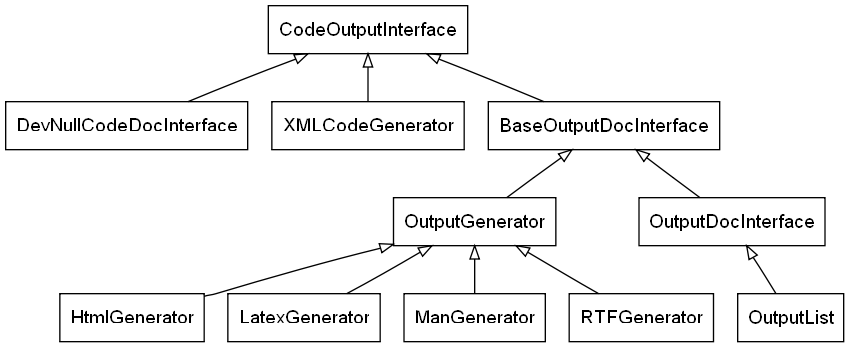
\includegraphics[width=0.8\textwidth]{images/doxy_objtree_our.png}
\caption{Графическое представление фрагмента иерархии полиморфных классов программы doxygen, полученное с использованием приложения crec путем анализа информации о типах времени выполнения.}
\label{fig:doxy_objtree_our}
\end{figure}

\begin{figure}[htb!]
\centering
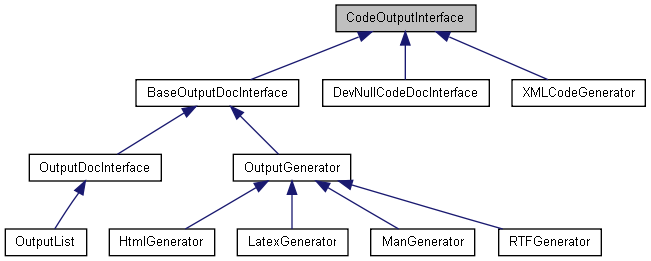
\includegraphics[width=0.8\textwidth]{images/doxy_objtree_doxy.png}
\caption{Графическое представление фрагмента иерархии полиморфных классов doxygen, полученное путем анализа исходного кода с помощью программы doxygen.}
\label{fig:doxy_objtree_doxy}
\end{figure}

Пример графического представления иерархии полиморфных классов, восстановленной с использованием приложения crec, приведен на рис. \ref{fig:doxy_objtree_our}. В качестве анализируемой программы использовалась система документирования исходных кодов doxygen. Одной из причин использования doxygen в качестве анализируемой программы является то, что doxygen распространяется с открытыми исходными кодами, что упрощает проверку корректности результатов восстановления. Также изучение исходных кодов doxygen показало, что в некоторых методах используется оператор \lstinline{dynamic_cast<>}, и поэтому для правильной работы этой программы она должна была быть скомпилирована с поддержкой информации о типах времени выполнения. Целью анализа являлось восстановление иерархии полиморфных классов. Для этого необходима информация о:
\begin{itemize}
\item Компиляторе, с использованием которого был получен исполняемый файл;
\item Формате RTTI структур, который используется этим компилятором.
%\item Извлечь RTTI структуры из исполнимого файла с использованием описанного выше алгоритма.
%\item Построить иерархию использованных в приложении полиморфных классов путем анализа извлеченных RTTI структур.
\end{itemize}

В результате применения методов, описанных в главе \ref{chapter:rtti_extraction}, было выяснено, что doxygen 1.5.8 для Windows скомпилирован компилятором MSVC, формат RTTI структур для которого был описан в главе \ref{chapter:rtti_in_msvc}. С использованием написанной на языке IDC части crec был проанализирован ассемблерный листинг. С использованием написанной на Си++ части crec была восстановлена полная иерархия полиморфных классов программы doxygen, состоящая из 444 классов. На рис. \ref{fig:doxy_objtree_our} приведено графическое представление фрагмента восстановленной иерархии полиморфных классов, а на рис. \ref{fig:doxy_objtree_doxy} --- графическое представление того же фрагмента, полученное путем анализа исходного кода. Как видно, фрагменты иерархии совпадают.

В результате сравнения иерархии полиморфных классов doxygen, построенной путем анализа исходного кода, с иерархией, восстановленной с использованием приложения crec, было выяснено, что эти иерархии совпадают.



\subsection{Программная реализация алгоритмов анализа, не использующих информацию о типах времени выполнения}
В приложении crec также были реализованы методы восстановления иерархий полиморфных классов для случая отсутствия информации о типах времени выполнения, описанные в главе \ref{chapter:reconstruction_without_rtti}. Извлечение информации, необходимой для построения ограничений с использованием утверждений \ref{stmt:first_good}-\ref{stmt:last_good}, производится в части crec, реализованной на языке IDC. Анализ извлеченной информации с использованием описанных в главе \ref{chapter:reconstruction_without_rtti} методов производится в части crec, реализованной на языке Си++. Результатом работы приложения crec является входной файл для утилиты dot из пакета GraphViz, как это описано в главе \ref{chapter:impl_with_rtti}.

\begin{figure}[htb!]
\centering
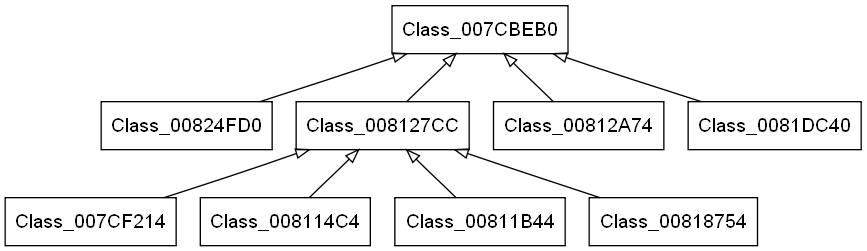
\includegraphics[width=0.8\textwidth]{images/doxy_objtree_nortti.png}
\caption{Графическое представление фрагмента иерархии полиморфных классов программы doxygen, полученное с использованием приложения crec без использования информации о типах времени выполнения.}
\label{fig:doxy_objtree_nortti}
\end{figure}

\begin{figure}[htb!]
\centering
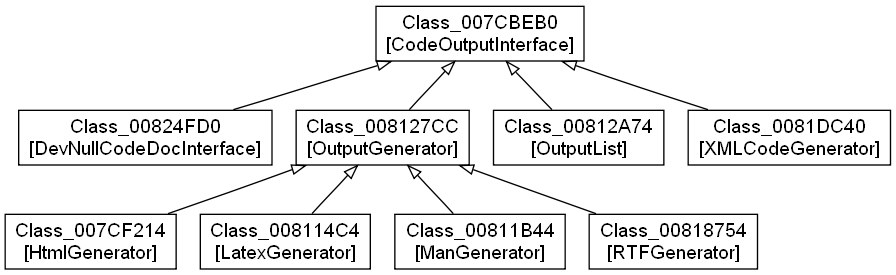
\includegraphics[width=0.8\textwidth]{images/doxy_objtree_nortti_label.png}
\caption{Графическое представление иерархии классов, представленной на рис. \ref{fig:doxy_objtree_nortti}, с сопоставленными классам реальными именами.}
\label{fig:doxy_objtree_nortti_label}
\end{figure}

Пример графического представления иерархии полиморфных классов, восстановленной с использованием приложения crec, представлен на рис. \ref{fig:doxy_objtree_nortti}. Также, как и в главе \ref{chapter:impl_with_rtti}, в качестве анализируемой программы использовалась система документирования исходных кодов doxygen. Анализируемый исполнимый файл был получен путем компиляции doxygen без поддержки информации о типах времени выполнения компилятором MSVC. При компиляции без информации о типах времени выполнения имена классов не попадает в исполнимый файл, и поэтому все классы на рис. \ref{fig:doxy_objtree_nortti} имеют автоматически сгенерированные имена.

Для проверки корректности восстановления система doxygen была скомпилирована еще раз с поддержкой информации о типах времени выполнения. Для исполнимого файла, полученного путем компиляции с использованием информации о типах времени выполнения, иерархия полиморфных классов была восстановлена так, как это описано в главе \ref{chapter:impl_with_rtti}. Путем сравнения виртуальных функций каждой таблице виртуальных функций из ассемблерного листинга исполнимого файла, полученного компиляцией без поддержки информации о типах времени выполнения, была поставлена в соответствие таблица виртуальных функций из ассемблерного листинга исполнимого файла, полученного компиляцией с поддержкой информации о типах времени выполнения. Таким образом, для каждой таблицы виртуальных функций из ассемблерного листинга исполнимого файла, полученного компиляцией без поддержки информации о типах времени выполнения, было получено имя соответствующего ей класса. На рис. \ref{fig:doxy_objtree_nortti_label} представлен фрагмент иерархии, соответствующий представленному на рис. \ref{fig:doxy_objtree_nortti} фрагменту иерархии, но с сопоставленными классам реальными именами.

Представленный на рис. \ref{fig:doxy_objtree_nortti_label} восстановленный фрагмент иерархии соответствует фрагменту, изображенному на рис. \ref{fig:doxy_objtree_doxy}. Как видно, фрагменты иерархии отличаются. Это объясняется тем, что классы \lstinline{BaseOutputDocInterface} и \lstinline{OutputDocInterface}, присутствующие в фрагменте иерархии, изображенном на рис. \ref{fig:doxy_objtree_doxy}, не перекрывают унаследованные ими виртуальные функции, а лишь добавляют новые чисто виртуальные функции, и потому компилятором для этих классов не была сгенерирована таблица виртуальных функций.

В результате сравнения иерархии полиморфных классов doxygen, восстановленной с помощью приложения crec без использования информации о типах времени выполнения, с иерархией, построенной путем анализа исходного кода, было выяснено, что восстановление иерархии было произведено корректно.















\newpage
\section*{Заключение}
\addcontentsline{toc}{section}{Заключение}
В данной работе были представлены методы автоматического восстановления объектных структур данных из низкоуровневого представления программ на языке Си++. Так как программа на языке Си++ может быть скомпилирована как с поддержкой, так и без поддержки информации о типах времени выполнения, то были рассмотрены оба случая.

Формат информации о типах времени выполнения зависит от используемого компилятора. Были рассмотрены форматы, используемые компиляторами GCC и MSVC. Для этих компиляторов также были рассмотрены основные положения используемых ими бинарных интерфейсов приложений, связанные с реализацией виртуальных функций. Анализ бинарных интерфейсов приложений показал, что задача поиска информации о типах времени выполнения сводится к задаче поиска таблиц виртуальных функций. Был представлен алгоритм поиска таблиц виртуальных функций, и метод восстановления иерархий классов, использующий этот алгоритм для локализации информации о типах времени выполнения.

Для случая отсутствия информации о типах времени выполнения был предложен метод поэтапного восстановления отношения наследования. Были рассмотрены правила языка программирования Си++ и положения бинарных интерфейсов приложений, используемых компиляторами GCC и MSVC, связанные с множественным наследованием. Анализ этих правил показал, что при отсутствии виртуальных деструкторов, множественное наследование может быть корректно заменено одиночным.

Было показано, что отношение наследования на множестве классов можно расширить на множество таблиц виртуальных функций, и что при этом наследование на множестве таблиц виртуальных функций является одиночным. Для восстановления одиночного наследования был разработан метод, основывающийся на анализе:
\begin{itemize}
\item Таблиц виртуальных функций;
\item Параметров виртуальных функций;
\item Вызовов виртуальных функций;
\item Виртуальных деструкторов.
\end{itemize}

Для восстановления множественного наследования был предложен метод объединения таблиц виртуальных функций, принадлежащих одному классу, и модификации деревьев одиночного наследования на множестве таблиц виртуальных функций, основывающийся на анализе виртуальных деструкторов.

Было разработано приложение crec, в котором были реализованы предложенные методы восстановления объектных структур данных как для случая присутствия информации о типах времени выполнения, так и для случая ее отсутствия. Приложение crec было протестировано на системе документирования исходных кодов doxygen, и были получены положительные результаты. В случае присутствия информации о типах времени выполнения иерархия полиморфных классов и таблицы виртуальных функций были восстановлены точно и полностью. В случае отсутствия информации о типах времени выполнения иерархия полиморфных классов была восстановлено корректно, с точностью до замены множественного наследования одиночным и удаления некоторых классов, для которых компилятором не были сгенерированы таблицы виртуальных функций.









\newpage

% this is really retarded...

\renewcommand{\appendixtocname}{Приложение А. Список используемых терминов и обозначений}
%\renewcommand{\appendixpagename}{}

\appendix
%\appendixpage
\addappheadtotoc
\section*{Приложение А. Список используемых терминов и обозначений}
К сожалению, термины в области программирования не устоялись. В разных переводах, и в различных работах на русском языке, наблюдаются существенные рассогласования. Поэтому здесь приведены значения используемых в данной работе терминов. Все термины, имеющие отношения к языкам программирования, такие как {\it класс}, {\it объект}, или {\it функция}, рассматриваются в данной работе в применении к языку программирования Си++.

\begin{itemize}
\item {\it Абстрактный класс} (англ. {\it abstract class}) --- класс, содержащий хотя бы одну {\it чисто виртуальную функцию}.
\item {\it Адаптер} (англ. {\it thunk}) --- дополнительный код, сгенерированный компилятором, выполняющий преобразование (например, типов), и передающий управление какой-либо функции с использованием инструкции безусловного перехода.
\item {\it Базовый класс} (англ. {\it base class}). Класс \lstinline{B} является базовым классом для класса \lstinline{D}, если он является {\it непосредственным базовым классом} для класса \lstinline{D}, или {\it непосредственным базовым классом} для одного из базовых классов класса \lstinline{D} \cite{cpp03}. %[10]
\item {\it Бинарный интерфейс приложений} (англ. {\it application binary interface} ) --- набор конфигураций среды разработки и компилятора, гарантирующих бинарную совместимость разрабатываемых приложений. Бинарный интерфейс приложений определяет взаимодействие на низком уровне между приложениями, между компонентами приложения, между приложением и библиотеками, и между приложением и операционной системой на используемой платформе.
\item {\it Виртуальная функция} (англ. {\it virtual function}) --- метод класса, который может быть переопределён в производных классах так, что конкретная реализация метода для вызова будет определяться во время выполнения программы. В языке программирования Си++ виртуальные функции определяются с ключевым словом \lstinline{virtual} \cite{stroustrup97ru}.
\item {\it Виртуальный метод} (англ. {\it virtual method}) --- см. {\it виртуальная функция}.
\item {\it Встраивание} (англ. {\it inline expansion}) --- оптимизация, при которой вызов функции заменяется на подстановку копии ее тела.
\item {\it Декорирование имен} (англ. {\it name mangling}) --- декорирование имен добавляет дополнительную информацию к имени функций, структур, классов, и других типов данных, чтобы избежать конфликтов на этапе {\it компоновки} программы. Разные компиляторы используют разные схемы декорирования имен.
\item {\it Динамический полиморфизм} (англ. {\it dynamic polymorphism}) --- форма {\it полиморфизма}, подразумевающая выбор необходимой операции обработки данных на этапе выполнения программы, то есть с использованием {\it позднего связывания}. В языке Си++ динамический полиморфизм реализуется системой {\it виртуальных функций}.
\item {\it Динамическое связывание} (англ. {\it dynamic binding}) --- определение реализации вызываемого метода во время выполнения программы на основании фактического типа объекта (или объектов), для которого был вызван этот метод.
\item {\it Информация о типах времени выполнения} (англ. {\it run-time type information})--- стандартизованный интерфейс, с помощью которого программы на языке Си++, использующим указатели или ссылки на базовые классы, могут выяснять фактические типы объектов производных классов, к которым относятся эти указатели или ссылки \cite{lippman07ru}. Реализации информации о типах времени выполнения в разных компиляторах существенно отличаются.
\item {\it Компоновка} (англ. {\it linking}) --- процесс создания исполняемого модуля программы из одного или нескольких объектных модулей, полученных в результате компиляции исходных файлов программы.
\item {\it Наследник} (англ. {\it child class}) --- см. {\it производный класс}.
\item {\it Непосредственный базовый класс} (англ. {\it direct base class}). Класс \lstinline{B} является непосредственным базовым классом для класса \lstinline{D}, если в соответствующей программе на языке Си++ класс \lstinline{B} присутствует в списке базовых классов для класса \lstinline{D} \cite{cpp03}.%[10]
\item {\it Обратное проектирование} (англ. {\it reverse engeneering}) --- процесс извлечения информации о строении и принципах работы системы путем анализа ее функций, структуры, и поведения. В применении к программному обеспечению целью обратного проектирования является повышение уровня абстракции представления программ.
\item {\it Перегрузка функций} (англ. {\it function overloading}) --- возможность языка программирования поддерживать одновременное существование в одной области видимости нескольких различных вариантов функции, имеющих одно и то же имя, но различающихся типами параметров, к которым она применяется.
\item {\it Перекрытие методов} (англ. {\it method overriding}) --- особенность языка программирования, позволяющая производному классу заменить реализацию {\it виртуального метода} базового класса.
\item {\it Позднее связывание} (англ. {\it late binding}) --- см. {\it динамическое связывание}.
\item {\it Полиморфизм} (англ. {\it polymorphism}) --- в применении к языкам программирования, это возможность работать с данными разных типов с использованием одного и того же интерфейса.
\item {\it Полиморфный класс} (англ. {\it polymorphic class}) --- класс, имеющий хотя бы одну {\it виртуальную функцию} \cite{stroustrup97ru}.
\item {\it Предок} (англ. parent class) --- см. {\it базовый класс}.
\item {\it Производный класс} (англ. {\it derived class}). Класс \lstinline{D} является производным от класса \lstinline{B} классом, тогда и только тогда, когда класс \lstinline{B} является {\it базовым классом} для класса \lstinline{D}.
\item {\it Соглашение о вызовах} (англ. {\it calling conventions}) --- часть {\it бинарного интерфейса приложений}, которая регламентирует технические особенности вызова подпрограмм, передачи параметров, возврата из подпрограмм и передачи результата вычислений в точку вызова.
\item {\it Статический полиморфизм} (англ. {\it static polymorphism}) --- форма {\it полиморфизма}, подразумевающая выбор необходимой операции обработки данных на этапе компиляции программы, то есть с использованием {\it статического связывания}. Примерами статического полиморфизма в языке Си++ являются {\it шаблоны} и {\it перегруженные функции}.
\item {\it Статическое связывание} (англ. {\it static binding}) --- в применении к вызовам функций в программе на языке Си++, применение статического связывания подразумевает, что реализация вызываемой функции известна во время компиляции программы. Это в частности означает, что вызываемая функция может быть {\it встроена} в код вызывающей функции.
\item {\it Стековый фрейм} (англ. {\it stack frame}) --- зависимая от используемой платформы и компилятора структура данных, хранящая информацию о состоянии выполняемой подпрограммы.
\item {\it Таблица виртуальных функций} (англ. {\it virtual function table}) --- система, используемая в языках программирования для реализации {\it динамического связывания}. При использовании таблицы виртуальных функций, каждый объект {\it полиморфного класса} содержит указатель на соответствующую классу таблицу виртуальных функций, включающую адреса всех {\it виртуальных методов} класса \cite{stroustrup90ru}.
%\item {\it Объединение} (англ. union) --- тип данных \lstinline{union} языка Си++.
\item {\it Чисто виртуальная функция} (англ. {\it pure virtual function}) --- {\it виртуальная функция} без реализации. Реализации ее, возможно, различные, могут содержаться в производных классах.
%\item {\it Шаблоны} (англ. {\it templates}) — средство языка C++, предназначенное для реализации обобщенных алгоритмов, без привязки к некоторым параметрам, таким как типы данных, размеры буферов, значения по умолчанию, и т.п.
%\item {\it Curiously Recurring Template Pattern} --- прием, при использовании которого объявляемый класс \lstinline{Derived} наследуется от шаблонного класса, инстанциированного с \lstinline{Derived} в качестве одного из параметров шаблона. Чаще всего используется для реализации формы статического полиморфизма, схожей с используемой в системе виртуальных функций языка Си++, но использующей статическое связывание.
\end{itemize}


Ниже перечислены основные обозначения, используемые в данной работе.
\begin{itemize}
\item $R^{-1}$ --- отношение, обратное к $R \subseteq X \times X$. $R^{-1} = \{(y, x) | (x, y) \in R \}$.
\item $R^+$ --- транзитивное замыкание бинарного отношения $R \subseteq X \times X$. $R^+$ является наименьшим транзитивным отношением на множестве $X$, включающим $R$.
\item $R^=$ --- рефлексивное замыкание бинарного отношения $R \subseteq X \times X$. $R^=~=~R \cup \{ (x, x) | x \in X \}$.
\item $R^{\ne}$ --- рефлексивное сужение бинарного отношения $R \subseteq X \times X$. $R^{\ne}~=~R~\setminus~\{ (x, x) | x \in X \}$.
%\item $R^s$ --- симметричное замыкание бинарного отношения $R \subseteq X \times X$. $R^s~=~{(x, y) | (x, y) \in R \vee (y, x) \in R}$.
\item $S \circ R$ --- композиция бинарных отношений $R, S \subseteq X \times X$, определенная как $S \circ R = \{(x, z) | \exists y \in X: (x, y) \in R \wedge (y, z) \in S\}$.
\item $|X|$ --- мощность множества $X$.
\item $\nG(X)$ --- множество всевозможных графов $G = (X, E)$.
\item $\nT(X)$ --- множество всевозможных деревьев $T = (X, E)$.
\item $\nT^R(X)$ --- множество всевозможных корневых деревьев $T = (X, E, r)$, где $r \in X$ --- корень дерева.
\item $R[Y]$ --- сужение отношения $R \subseteq X \times X$ на множество $Y \subseteq X$, то есть $R[Y] = R \cap (Y \times Y)$.
\item $T[Y]$ --- сужение дерева $T = (X, E)$ на множество вершин $Y \subseteq X$, то есть $T[Y] = (Y, E[Y])$.
\item $T[\nT]$ --- дерево $T' = (X, E)$, соответствующее корневому дереву $T = (X, E, r)$.
\item $\gC_{\bP}$ --- множество всех полиморфных классов программы на языке Си++ $\bP$.
\item $\leftarrow_{\bP}$ --- бинарное отношение непосредственного наследования, определенное на множестве $\gC_{\bP}$ для программы на языке Си++ $\bP$. Для любых двух классов $B, D \in \gC_{\bP}$, $B~\leftarrow_{\bP}~D \enspace \Longleftrightarrow \enspace B \enspace$ является {\it непосредственным базовым классом} для $\enspace D$.
\item $\lhd_{\bP} = \enspace \leftarrow_{\bP}^+$ --- бинарное отношение наследования, определенное на множестве $\gC_{\bP}$ для программы на языке Си++ $\bP$. Для любых двух классов $B, D \in \gC_{\bP}$, $B~\lhd_{\bP}~D \enspace \Longleftrightarrow \enspace B \enspace \text{является {\it базовым классом} для} \enspace D$. Это обозначение соответствует определению базового класса, данному выше.
\end{itemize}

\newpage
\raggedright
\addcontentsline{toc}{section}{Список литературы}
\begin{thebibliography}{99}
\bibitem{boldewin06}
Boldewin F. The big SoftICE how-to [PDF] (\url{http://www.reconstructer.org/papers/The%20big%20SoftICE%20howto.pdf}).

\bibitem{dolgova08}
Dolgova K., Chernov A. Automatic Type Reconstruction in Disassembled C Programs // 15th Working Conference on Reverse Engineering. 2008. P. 202-206.

\bibitem{emmerik04}
Emmerik M. V., Waddington T. Using a Decompiler for Real-World Source Recovery // 11th Working Conference on Reverse Engineering. 2004. P. 27-36.

\bibitem{emmerik07}
Emmerik M. V. Static Single Assignment for Decompilation [PDF] (\url{http://vanemmerikfamily.com/mike/master.pdf}).
%A thesis submitted for the degree of Doctor of Philosophy at The University of Queensland, 2007.

\bibitem{gray94}
Gray J. C++: {\begin{CJK*}{UTF8}{ipam}水面下の仕組み\end{CJK*}} [HTML] (\url{http://www.microsoft.com/japan/msdn/vs_previous/visualc/techmat/feature/jangrayhood/}).
%Gray J. C++: Under the Hood [HTML] (\url{http://msdn.microsoft.com/archive/en-us/dnarvc/html/jangrayhood.asp}).

\bibitem{kochhar02}
Kochhar V. How a C++ compiler implements exception handling [HTML] (\url{http://www.codeproject.com/KB/cpp/exceptionhandler.aspx}).

\bibitem{mycroft99}
Mycroft A. Type-Based Decompilation // 8th European Symposium on Programming Languages and Systems. 1999. P. 208-223.

\bibitem{palmer94}
Palmer C., Kershenbaum A. Representing trees in genetic algorithms // First IEEE Conference on Evolutionary Computation. 1994. P. 27-29.

\bibitem{sabanal07}
Sabanal P., Yason M. Reversing C++ // Black Hat DC. 2007.

\bibitem{seonghoon06}
Seonghoon K. Microsoft C++ Name Mangling Scheme [HTML] (\url{http://mearie.org/documents/mscmangle}).

\bibitem{skochinsky06}
Skochinsky I. Reversing Microsoft Visual C++ Part II: Classes, Methods and RTTI [HTML] (\url{http://www.openrce.org/articles/full_view/23}).

\bibitem{stroustrup93}
Stroustrup B. A history of C++: 1979–1991 // The second ACM SIGPLAN conference on History of programming languages. 1993. P. 271-297.

\bibitem{stroustrup97}
Stroustrup B. The C++ programming language 3rd edition. Massachusetts: Addison-Wesley, 1997. 1022 p.

\bibitem{wiener05}
Wiener R. Obfuscation and .NET // Journal of Object Technology. 2005. 4. N 4. P. 73-92.

\bibitem{lippman07ru}
Липпман С., Му Б., Лажойе Ж. Язык программирования C++, вводный курс, 4-е издание. М.: Вильямс, 2007. 896 с.

\bibitem{stroustrup97ru}
Строуструп Б. Язык программирования С++, специальное издание. М.: Бином, 2004. 1104 с.

\bibitem{stroustrup90ru}
Эллис М., Строуструп Б. Справочное руководство по языку программирования С++ с комментариями. Проект стандарта ANSI. M.: Мир, 1992. 445 с.

\bibitem{abi}
Application Binary Interface [HTML] (\url{http://en.wikipedia.org/wiki/Application_binary_interface}).

\bibitem{boomerang}
Boomerang. BSD licensed software [HTML] (\url{http://boomerang.sourceforge.net/}).

\bibitem{graphviz}
GraphViz. CPL licensed software [HTML] (\url{http://www.graphviz.org/}).

\bibitem{softicescripting}
IceX. A free SoftICE Plugin [HTML] (\url{http://mamaich.uni.cc/}).

\bibitem{idapro}
IDA Pro Disassembler. Proprietary software [HTML] (\url{http://www.hex-rays.com/idapro/}).

\bibitem{idapython}
IDAPython. A free IDA Pro plugin [HTML] (\url{http://www.d-dome.net/idapython}).

\bibitem{idarub}
IDARub. A free IDA Pro plugin [HTML] (\url{http://www.metasploit.com/users/spoonm/idarub/}).

\bibitem{cpp03}
ISO/IEC Standard 14882:2003. Programming languages - C++. New York: American National Standards Institute, 2003. 786 p.

\bibitem{gccabi}
Itanium C++ ABI, revision 1.86 [HTML] (\url{http://www.codesourcery.com/public/cxx-abi/abi.html}).

\bibitem{mfc}
Microsoft Foundation Class Library Reference [HTML] (\url{http://msdn.microsoft.com/en-us/library/d06h2x6e.aspx}).

\bibitem{ollydbg}
OllyDbg. Proprietary software [HTML] (\url{http://www.ollydbg.de/}).

\bibitem{ollypython}
OllyPython. A free OllyDbg plugin [HTML] (\url{http://code.google.com/p/ollypython/}).

\bibitem{polymorphism}
Polymorphism in object-oriented programming [HTML] (\url{http://en.wikipedia.org/wiki/Polymorphism_in_object-oriented_programming}).

\bibitem{qt}
Qt --- A cross-platform application and UI framework [HTML] (\url{http://www.qtsoftware.com/products/}).

\bibitem{wine}
Wine. LGPL licensed software [HTML] (\url{http://www.winehq.org}).

\bibitem{idaproproc}
Поддерживаемые типы процессоров IDA Pro - Interactive Disassembler [HTML] (\url{http://www.idapro.ru/description/proc/}).

\bibitem{idaproformats}
Поддерживаемые форматы входных файлов IDA Pro - Interactive Disassembler [HTML] (\url{http://www.idapro.ru/description/format/}).

\end{thebibliography}
























\end{document}



















